\documentclass[12pt]{amsart}

% PACKAGES
\usepackage{amsmath}
\usepackage{amssymb}
\usepackage{amsfonts}
\usepackage[alphabetic]{amsrefs}
\usepackage{amsthm}
\usepackage{enumitem}
\setlist[enumerate,1]{left=0pt,label=(\arabic*)}
%\usepackage{enumerate}
\usepackage{fullpage}
\usepackage{color}
\usepackage{graphicx}
\usepackage{wrapfig}
\usepackage{hyperref}
\usepackage{microtype}
\usepackage{correctmathalign}
\usepackage{tikz}
\usepackage{float}
\usepackage{caption}
\usepackage{quiver}
%\usepackage{lipsum}
%\hypersetup{linktoc = all, colorlinks = true, urlcolor = Blue, linkcolor = Red, citecolor = RoyalBlue}
%\usepackage[parfill]{parskip}


% COMMANDS 
\newcommand{\nc}{\newcommand}
\newcommand{\rc}{\renewcommand}
\nc{\on}{\operatorname}

% EDITING
\definecolor{red}{rgb}{1,0,0}
\definecolor{orange}{rgb}{1,0.5,0}
\definecolor{purple}{rgb}{.5,.2,.8}
\definecolor{blue}{rgb}{.2,.2,.8}
\definecolor{green}{rgb}{.4,.6,.4}
\definecolor{myorange}{RGB}{235, 129, 27}
\newcommand{\question}[1]{\noindent  \textcolor{red}{Question: #1}}
\newcommand{\todo}[1]{\noindent  \textcolor{blue}{To do: #1}}

% Editing line spacing
%\linespread{1.5}

% BLACKBOARD BOLD
\rc{\AA}{\mathbb{A}}	
\nc{\BB}{\mathbb{B}}	
\nc{\CC}{\mathbb{C}}	
\nc{\DD}{\mathbb{D}}	
\nc{\EE}{\mathbb{E}}	
\nc{\FF}{\mathbb{F}}	
\nc{\GG}{\mathbb{G}}	
\nc{\HH}{\mathbb{H}}	
\nc{\II}{\mathbb{I}}	
\nc{\JJ}{\mathbb{J}}	
\nc{\KK}{\mathbb{K}}	
\nc{\LL}{\mathbb{L}}	
\nc{\MM}{\mathbb{M}}	
\nc{\NN}{\mathbb{N}}	
\nc{\OO}{\mathbb{O}}	
\nc{\PP}{\mathbb{P}}	
\nc{\QQ}{\mathbb{Q}}	
\nc{\RR}{\mathbb{R}}	
\rc{\SS}{\mathbb{S}}	
\nc{\TT}{\mathbb{T}}	
\nc{\UU}{\mathbb{U}}	
\nc{\VV}{\mathbb{V}}	
\nc{\WW}{\mathbb{W}}	
\nc{\XX}{\mathbb{X}}	
\nc{\YY}{\mathbb{Y}}	
\nc{\ZZ}{\mathbb{Z}}	

% BOLD FACE
\nc{\bA}{\mathbf{A}}	
\nc{\bB}{\mathbf{B}}	
\nc{\bC}{\mathbf{C}}	
\nc{\bD}{\mathbf{D}}	
\nc{\bE}{\mathbf{E}}	
\nc{\bF}{\mathbf{F}}	
\nc{\bG}{\mathbf{G}}	
\nc{\bH}{\mathbf{H}}	
\nc{\bI}{\mathbf{I}}	
\nc{\bJ}{\mathbf{J}}	
\nc{\bK}{\mathbf{K}}	
\nc{\bL}{\mathbf{L}}	
\nc{\bM}{\mathbf{M}}	
\nc{\bN}{\mathbf{N}}	
\nc{\bO}{\mathbf{O}}	
\nc{\bP}{\mathbf{P}}	
\nc{\bQ}{\mathbf{Q}}	
\nc{\bR}{\mathbf{R}}	
\nc{\bS}{\mathbf{S}}	
\nc{\bT}{\mathbf{T}}	
\nc{\bU}{\mathbf{U}}	
\nc{\bV}{\mathbf{V}}	
\nc{\bW}{\mathbf{W}}	
\nc{\bX}{\mathbf{X}}	
\nc{\bY}{\mathbf{Y}}	
\nc{\bZ}{\mathbf{Z}}	

% CALLIGRAPHIC
\nc{\calA}{\mathcal{A}}	
\nc{\calB}{\mathcal{B}}	
\nc{\calC}{\mathcal{C}}	
\nc{\calD}{\mathcal{D}}	
\nc{\calE}{\mathcal{E}}	
\nc{\calF}{\mathcal{F}}	
\nc{\calG}{\mathcal{G}}	
\nc{\calH}{\mathcal{H}}	
\nc{\calI}{\mathcal{I}}	
\nc{\calJ}{\mathcal{J}}	
\nc{\calK}{\mathcal{K}}	
\nc{\calL}{\mathcal{L}}	
\nc{\calM}{\mathcal{M}}	
\nc{\calN}{\mathcal{N}}	
\nc{\calO}{\mathcal{O}}	
\nc{\calP}{\mathcal{P}}	
\nc{\calQ}{\mathcal{Q}}	
\nc{\calR}{\mathcal{R}}	
\nc{\calS}{\mathcal{S}}
\nc{\calT}{\mathcal{T}}	
\nc{\calU}{\mathcal{U}}	
\nc{\calV}{\mathcal{V}}	
\nc{\calW}{\mathcal{W}}
\nc{\calX}{\mathcal{X}}	
\nc{\calY}{\mathcal{Y}}	
\nc{\calZ}{\mathcal{Z}}

% LOWERCASE FRAK
\nc{\fraka}{\mathfrak{a}}
\nc{\frakb}{\mathfrak{b}}
\nc{\frakc}{\mathfrak{c}}
\nc{\frakd}{\mathfrak{d}}
\nc{\frake}{\mathfrak{e}}
\nc{\frakf}{\mathfrak{f}}
\nc{\frakg}{\mathfrak{g}}
\nc{\frakh}{\mathfrak{h}}
\nc{\fraki}{\mathfrak{i}}
\nc{\frakj}{\mathfrak{j}}
\nc{\frakk}{\mathfrak{k}}
\nc{\frakl}{\mathfrak{l}}
\nc{\frakm}{\mathfrak{m}}
\nc{\frakn}{\mathfrak{n}}
\nc{\frako}{\mathfrak{o}}
\nc{\frakp}{\mathfrak{p}}
\nc{\frakq}{\mathfrak{q}}
\nc{\frakr}{\mathfrak{r}}
\nc{\fraks}{\mathfrak{s}}
\nc{\frakt}{\mathfrak{t}}
\nc{\fraku}{\mathfrak{u}}
\nc{\frakv}{\mathfrak{v}}
\nc{\frakw}{\mathfrak{w}}
\nc{\frakx}{\mathfrak{x}}
\nc{\fraky}{\mathfrak{y}}
\nc{\frakz}{\mathfrak{z}}

% UPPERCASE FRAK
\nc{\frakA}{\mathfrak{A}}
\nc{\frakB}{\mathfrak{B}}
\nc{\frakC}{\mathfrak{C}}
\nc{\frakD}{\mathfrak{D}}
\nc{\frakE}{\mathfrak{E}}
\nc{\frakF}{\mathfrak{F}}
\nc{\frakG}{\mathfrak{G}}
\nc{\frakH}{\mathfrak{H}}
\nc{\frakI}{\mathfrak{I}}
\nc{\frakJ}{\mathfrak{J}}
\nc{\frakK}{\mathfrak{K}}
\nc{\frakL}{\mathfrak{L}}
\nc{\frakM}{\mathfrak{M}}
\nc{\frakN}{\mathfrak{N}}
\nc{\frakO}{\mathfrak{O}}
\nc{\frakP}{\mathfrak{P}}
\nc{\frakQ}{\mathfrak{Q}}
\nc{\frakR}{\mathfrak{R}}
\nc{\frakS}{\mathfrak{S}}
\nc{\frakT}{\mathfrak{T}}
\nc{\frakU}{\mathfrak{U}}
\nc{\frakV}{\mathfrak{V}}
\nc{\frakW}{\mathfrak{W}}
\nc{\frakX}{\mathfrak{X}}
\nc{\frakY}{\mathfrak{Y}}
\nc{\frakZ}{\mathfrak{Z}}

% OPERATORS
\nc{\Lie}{\on{Lie}}
\nc{\GL}{\on{GL}}
\nc{\PGL}{\on{PGL}}
\nc{\SL}{\on{SL}}
\nc{\Sp}{\on{Sp}}
\nc{\GSp}{\on{GSp}}
\nc{\SO}{\on{SO}}
\nc{\Or}{\on{O}}
\nc{\gl}{\on{\mathfrak{gl}}}
\rc{\sl}{\on{\mathfrak{sl}}}
\nc{\git}{/\!\!/}

\nc{\Mat}{\on{Mat}}
\nc{\Fun}{\on{Fun}}
\nc{\Aut}{\on{Aut}}
\nc{\End}{\on{End}}
\nc{\Hom}{\on{Hom}}
\nc{\Sym}{\on{Sym}}
\nc{\Span}{\on{span}}
\nc{\Irr}{\on{Irr}}
\nc{\Uch}{\on{Uch}}
\nc{\Type}{\on{Type}}
\nc{\Spec}{\on{Spec}}

\nc{\Ind}{\on{Ind}}
\nc{\Res}{\on{Res}}
\nc{\stab}{\on{stab}}
\nc{\orb}{\on{orb}}
\rc{\ker}{\on{ker}}
\nc{\im}{\on{im}}
\nc{\tr}{\on{tr}}
\nc{\ord}{\on{ord}}
\nc{\Tor}{\on{Tor}}
\nc{\Ad}{\on{Ad}}

\nc{\Id}{\on{Id}}
\nc{\Log}{\on{Log}}
\nc{\Exp}{\on{Exp}}
\nc{\Frac}{\on{Frac}}
\nc{\diag}{\on{diag}}
\nc{\D}{\on{D}}

% MATHRM
\nc{\St}{\mathrm{St}}
\nc{\triv}{\mathrm{triv}}
\nc{\sgn}{\mathrm{sgn}}
\nc{\reg}{\mathrm{reg}}
\nc{\rank}{\mathrm{rank}}
\nc{\op}{\mathrm{op}}
\nc{\ad}{\mathrm{ad}}
\rc{\ss}{\mathrm{ss}}
\nc{\HLV}{\mathrm{HLV}}

% ENVIRONMENTS
\theoremstyle{plain}
\newtheorem{theorem}{Theorem}[subsection]
\newtheorem{definition}[theorem]{Definition}
\newtheorem{corollary}[theorem]{Corollary}
\newtheorem{lemma}[theorem]{Lemma}
\newtheorem{proposition}[theorem]{Proposition}
\newtheorem{claim}[theorem]{Claim}
\newtheorem{example}[theorem]{Example}
\newtheorem{remark}[theorem]{Remark}

% CONE PLOTTING
\usepackage{graphicx} % For including graphics
\usepackage{subcaption} % For subfigures
\renewcommand{\thesubfigure}{\arabic{subfigure}}
\usepackage{tikz}
\usepackage{amsmath}
\usepackage{pgfplots}
\pgfplotsset{compat=1.17}
\usepackage{tikz,tikz-3dplot}
\tdplotsetmaincoords{80}{45}
\tdplotsetrotatedcoords{-90}{180}{-90}

%% style for surfaces
\tikzset{surface/.style={draw=gray!70!black, fill=gray!40!white, fill opacity=.6}}

%% macros to draw back and front of cones
%% optional first argument is styling; others are z, radius, side offset (in degrees)
\newcommand{\coneback}[4][]{
  %% start at the correct point on the circle, draw the arc, then draw to the origin of the diagram, then close the path
  \draw[canvas is xy plane at z=#2, #1] (45-#4:#3) arc (45-#4:225+#4:#3) -- (O) --cycle;
}
\newcommand{\conefront}[4][]{
  \draw[canvas is xy plane at z=#2, #1] (45-#4:#3) arc (45-#4:-135+#4:#3) -- (O) --cycle;
}

\allowdisplaybreaks

\begin{document}

\pagenumbering{roman}

\begin{center}

\includegraphics[width=10cm]{../images/UQLogo.jpg} \\ 
\vspace{3cm}
{\LARGE\textsc{Toric Varieties}} \\
%\vspace{0.1cm}
%{\LARGE\textsc{Varieties}} \\
\vspace{0.5cm}
{\textsc{Declan Fletcher}} \\
\vspace{8cm}
%{\textsc{Mid-year Review, July 2024}} \\
{\textsc{ Bachelor of Mathematics (Honours)}} \\
\vspace{1cm}
{\textsc{Supervisor: \href{https://sites.google.com/site/masoudkomi/home}{Masoud Kamgarpour}}} \\
{\textsc{Co-Supervisor: \href{https://sites.google.com/site/yangzhang139/home}{Yang Zhang}}} \\
\vspace{1cm}
{\textsc{\href{https://www.uq.edu.au/}{The University of Queensland}}} \\
{\textsc{\href{https://smp.uq.edu.au/}{School of Mathematics and Physics}}}
\end{center}

\newpage
\tableofcontents

\newpage
\pagenumbering{arabic}
\section*{Introduction}\label{chapter:introduction}
\addtocontents{toc}{\protect\setcounter{tocdepth}{1}}
\subsection*{Revolutions in geometry}
Mathematicians have studied geometry since ancient times.
Around 300 BC, the Ancient Greek mathematician Euclid wrote his textbook the Elements.
The axiomatisation of geometry in the Elements was groundbreaking, and it remained the most important textbook on geometry for hundreds of years.
Euclid often employed straight-edge and compass arguments to construct geometric shapes.
In these arguments, one is allowed to draw circles of fixed radii with a compass, and straight lines using the straight-edge, but distances and angles cannot be measured.

\begin{figure}[H]
\begin{center}
\begin{minipage}{0.22\textwidth} % First diagram
    \begin{tikzpicture}[scale=0.9]
    \pgfmathsetmacro{\sqrttree}{sqrt(3)}
    \draw (-2,0) -- (2,0);
    %\draw (-0.5,0) circle (1);
    %\draw (0.5,0) circle (1);
    %\draw (1.19282, -1.2) -- (-0.19282, 1.2);
    %\draw (-1.19282, -1.2) -- (0.19282, 1.2);
    \end{tikzpicture}
\end{minipage}%
\hfill % Adds space between the diagrams
\begin{minipage}{0.22\textwidth} % Second diagram
    \begin{tikzpicture}[scale=0.9]
    \pgfmathsetmacro{\sqrttree}{sqrt(3)}
    \draw (-2,0) -- (2,0);
    \draw (-0.5,0) circle (1);
%    \fill (-0.5,0) circle (1.5pt);
    %\draw (0.5,0) circle (1);
    %\draw (1.19282, -1.2) -- (-0.19282, 1.2);
    %\draw (-1.19282, -1.2) -- (0.19282, 1.2);
    \end{tikzpicture}
\end{minipage}%
\hfill
\begin{minipage}{0.22\textwidth} % Third diagram
    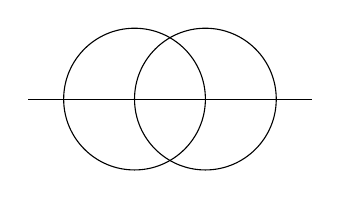
\begin{tikzpicture}[scale=0.9]
    \pgfmathsetmacro{\sqrttree}{sqrt(3)}
    \draw (-2,0) -- (2,0);
    \draw (-0.5,0) circle (1);
%    \fill (-0.5,0) circle (1.5pt);
    \draw (0.5,0) circle (1);
%    \fill (0.5,0) circle (1.5pt);
    %\draw (1.19282, -1.2) -- (-0.19282, 1.2);
    %\draw (-1.19282, -1.2) -- (0.19282, 1.2);
    \end{tikzpicture}
\end{minipage}%
\hfill
\begin{minipage}{0.22\textwidth} % Fourth diagram
    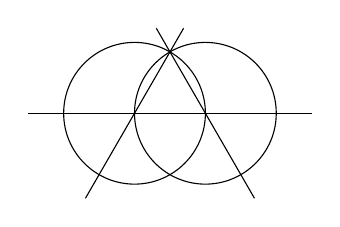
\begin{tikzpicture}[scale=0.9]
    \pgfmathsetmacro{\sqrttree}{sqrt(3)}
    \draw (-2,0) -- (2,0);
    \draw (-0.5,0) circle (1);
%    \fill (-0.5,0) circle (1.5pt);
    \draw (0.5,0) circle (1);
%    \fill (0.5,0) circle (1.5pt);
    \draw (1.19282, -1.2) -- (-0.19282, 1.2);
    \draw (-1.19282, -1.2) -- (0.19282, 1.2);
    \end{tikzpicture}
\end{minipage}
\end{center}
\caption{Constructing an equilateral triangle by straight-edge and compass.}
\end{figure}
\noindent
Although Euclid's work was groundbreaking, geometry progressed immensely over the centuries.

In the $17^\text{th}$ century, French mathematicians Descartes and Fermat independently discovered coordinate geometry.
They realised that geometric points could be described by $(x, y)$ coordinates.
Further, shapes such as curves and lines could be described by algebraic equations.
This meant that instead of using concrete constructive arguments like Euclid, Descartes and Fermat could reason about geometry using algebra.

At the start of the $20^\text{th}$ century, abstract algebra was beginning to be developed by David Hilbert and Emmy Noether.
One kind of object studied in abstract algebra is a ring---these are spaces where addition and multiplication are defined.
Familiar examples of rings include the integers $\ZZ$ and polynomial rings like $\CC[X]$.
Hilbert understood that rings could be used to understand geometry.
The idea is that given a geometric space, one can associate a ring of functions on the space:
\begin{align*}
%\left\{
\begin{array}{c}
	\text{Geometric space} \\
	V
\end{array}
%\right\} 
\rightsquigarrow
%\left\{
\begin{array}{c}
	\text{Function ring} \\
	\Fun(V, \CC)
\end{array}
%\right\}.
\end{align*}
In other words, geometry determines algebra.
The algebraic properties of $\Fun(V, \CC)$ tell us geometric properties of the space $V$.
The more surprising insight is that algebra determines geometry.
In other words, given a ring of functions $\Fun(V, \CC)$, we can determine the space $V$ that has this ring of functions:
\begin{align*}
%\left\{
\begin{array}{c}
	\text{Geometric space} \\
	 V
\end{array}
%\right\} 
\scalebox{-1}[1]{$\rightsquigarrow$}
%\left\{
\begin{array}{c}
	\text{Function ring} \\
	\Fun(V, \CC)
\end{array}
%\right\}.
\end{align*}
Thus, algebra determines geometry.
Hilbert's great insight was that studying geometry and algebra are equivalent.
The study of geometry using techniques of abstract algebra is called algebraic geometry.

\newpage
\subsection*{Algebraic geometry}
Algebraic geometry studies spaces called algebraic varieties.
These are sets of solutions $(a_1, \ldots, a_n)$ in $\CC^n$ to polynomial equations
$$f_1(a_1, \ldots, a_n) = 0, \qquad \ldots, \qquad f_s(a_1, \ldots, a_n) = 0,$$
where $f_1, \ldots, f_s$ are  $n$-variable polynomials in $\CC[X_1, \ldots, X_n]$.
Familiar examples include the circle and sphere (see examples (1) and (2) in Figure \ref{figure:fourvarieties}).
Cubic curves and cones provide other examples (see examples (3) and (4) in Figure \ref{figure:fourvarieties}).

\begin{figure}[H]
    \centering
    \begin{subfigure}[t]{0.23\textwidth}
        \centering
	\vspace{-0cm}
        
\begin{tikzpicture}
        \draw[ultra thick, myorange, samples=100, smooth] 
        plot[domain=0:360] ({cos(\x)}, {sin(\x)});
        \end{tikzpicture}
	  \vspace{0.2cm}
        \caption{$x^2 + y^2 = 1$}
    \end{subfigure}
    \hfill
    \begin{subfigure}[t]{0.23\textwidth}
        \centering
	\vspace*{-0.8cm}
        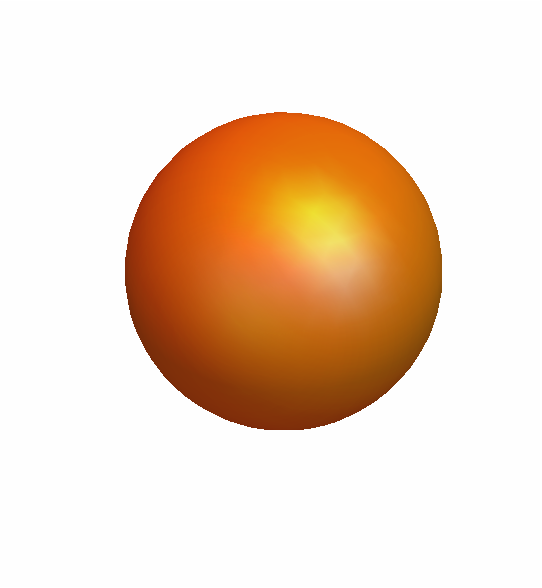
\includegraphics[width=\linewidth]{../images/orange_sphere}
	\vspace{-1.5cm}
        \caption{$x^2 + y^2 + z^2 = 1$}
    \end{subfigure}
    \hfill
    \begin{subfigure}[t]{0.23\textwidth}
        \centering
        \vspace{-0cm} % Adjust vertical space if needed
        
\begin{tikzpicture}
          \draw[ultra thick, myorange, samples=100, smooth, domain=-2:0.65, variable=\x] 
            plot ({\x}, {sqrt((\x)^3 + 2*(\x)^2)});
          \draw[ultra thick, myorange, samples=100, smooth, domain=-2:0.65, variable=\x] 
            plot ({\x}, {-sqrt((\x)^3 + 2*(\x)^2)});
        \end{tikzpicture}
	 \vspace{0.1cm}
        \caption{$y^2 = x^3 + 2x^2$}
    \end{subfigure}
    \hfill
    \begin{subfigure}[t]{0.23\textwidth}
        \centering
        \vspace{-0.5cm} % Adjust vertical space for this subfigure
        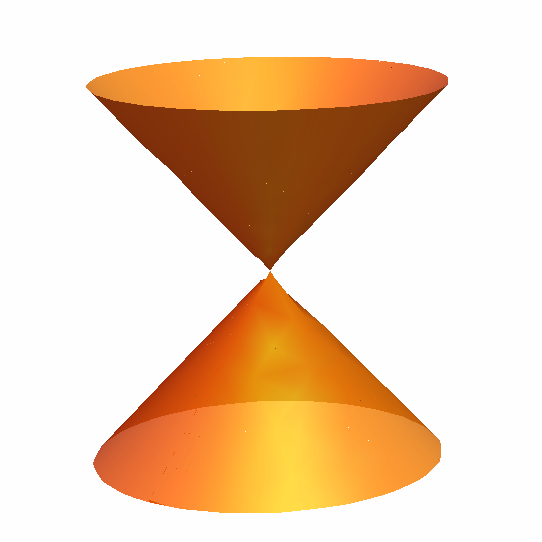
\includegraphics[width=0.8 \linewidth]{../images/orange_cone}
        \vspace{-0.3cm} % Adjust space below the image
        \caption{$xy = z^2$}
    \end{subfigure}
    \caption{Four examples of varieties.}
	\label{figure:fourvarieties}
\end{figure}

Examples (3) and (4) in Figure \ref{figure:fourvarieties} demonstrate that varieties may have singularities;
these are points where a variety ``crosses itself" or is ``pinched."
The presence of singularities in varieties is one of the key differences between algebraic geometry and differential geometry; indeed, in differential geometry, one studies smooth manifolds which by assumption have no singularities.
Singularities are related to tangent spaces of varieties, and singularities arise when the dimension of the tangent space is ``too large."

To study affine varieties using abstract algebra, we associate algebraic objects to varieties.
To begin with, we study algebraic varieties using polynomial function $\CC[X_1, \ldots, X_n]$.
Associated to a variety $V$ is the ideal of functions vanishing on $V$, which is denoted $\bI(V)$.
Using this, we can define the coordinate ring of $V$, 
$$\CC[V] := \CC[X_1, \ldots, X_n] / \bI(V),$$
which can be considered the ring of polynomial functions on $V$.
Thus, we have associated an algebraic object with the variety $V$.
It turns out that the relationship between algebra and geometry is very tight;
in fact, the ring $\CC[V]$ determines the variety $V$ up to isomorphism.
In this sense, the coordinate ring $\CC[V]$ is not just an algebraic shadow of $V$, but in fact, an equivalent object.

Given the equivalence of geometry and algebra, any geometric property we may be interested in should be able to be understood using algebra.
In Chapter \ref{chapter:algebraicsets} and Chapter 2 \ref{chapter:affinevarieties}, we study some geometric properties of varieties and the algebraic counterparts.
Key considerations of this kind include:
\begin{enumerate}
\item Irreducibility of algebraic sets corresponding to coordinate rings being integral domains.
\item The correspondence between maps between algebraic sets and algebra homomorphisms of coordinate rings.
\item The relationship between open sets of algebraic sets and localisation of coordinate rings.
\item Formalising the bijection between points in varieties and maximal ideals in coordinate rings by defining the maximal spectrum.
\item Characterising the tangent space of a variety using maximal ideals in the coordinate ring.
\end{enumerate}

\newpage
\subsection*{Toric varieties}





\newpage
\subsection*{Geometric invariant theory}




\newpage
\subsection*{Goals and structure of this thesis}
The main goal of this thesis is to prove that when $V$ is a rational representation of a torus $T$, the GIT quotient $V \git T$ is an affine toric variety whose cone can be computed.
To achieve this, we build up the preqrequisite theory concerning affine varieties and toric varieties which is needed.
We first explore the basic theory of algebraic sets and affine varieties in Chapter \ref{chapter:algebraicsets} and Chapter \ref{chapter:affinevarieties}, respectively.
Next, we delve into the convex geometry of cones in Chapter \ref{chapter:convexgeometry}.
Our understanding of affine varieties and convex geometry is applied in Chapter \ref{chapter:affinetoricvarieties} to studying affine toric varieties.
Finally, in Chapter \ref{chapter:gitquotientsastoricvarieties}, we show $V \git T$ is a toric variety.

Each chapter in this thesis is shown with its main object of study in the diagram below.
We note the dependency of chapters by writing an arrow Chapter $i$ $\to$ Chapter $j$ if Chapter $i$ should be read before Chapter $j$.
%% https://q.uiver.app/#q=WzAsNSxbMCwwLCJcXHRleHR7Q2hhcHRlciAyfSJdLFswLDEsIlxcdGV4dHtDaGFwdGVyIDN9Il0sWzEsMCwiXFx0ZXh0e0NoYXB0ZXIgNH0iXSxbMSwxLCJcXHRleHR7Q2hhcHRlciA1fSJdLFsxLDIsIlxcdGV4dHtDaGFwdGVyIDZ9Il0sWzAsMV0sWzIsM10sWzEsM10sWzMsNF1d
%\[\begin{tikzcd}
%	{\text{Chapter \ref{chapter:algebraicsets}}} & {\text{Chapter \ref{chapter:convexgeometry}}} \\
%	{\text{Chapter \ref{chapter:affinevarieties}}} & {\text{Chapter \ref{chapter:affinetoricvarieties}}} \\
%	& {\text{Chapter \ref{chapter:gitquotientsastoricvarieties}}}
%	\arrow[from=1-1, to=2-1]
%	\arrow[from=1-2, to=2-2]
%	\arrow[from=2-1, to=2-2]
%	\arrow[from=2-2, to=3-2]
%\end{tikzcd}\]
%% https://q.uiver.app/#q=WzAsNSxbMCwwLCJcXHRleHR7Q2guIDJ9IFxcXFwgXFx0ZXh0e0FsZ2VicmFpYyBzZXRzfSBcXFxcIFYiXSxbMCwxLCJcXHRleHR7Q2guIDN9IFxcXFwgXFx0ZXh0e0FmZmluZSB2YXJpZXRpZXN9IFxcXFwgXFxTcGVjKEEpIl0sWzEsMCwiXFx0ZXh0e0NoLiA0fSBcXFxcIFxcdGV4dHtDb252ZXggY29uZXN9IFxcXFwgXFxzaWdtYSJdLFsxLDEsIlxcdGV4dHtDaC4gNX0gXFxcXCBcXHRleHR7VG9yaWMgdmFyaWV0aWVzfSBcXFxcIFVfXFxzaWdtYSJdLFsxLDIsIlxcdGV4dHtDaC4gNn0gXFxcXCBcXHRleHR7VG9ydXMgcXVvdGllbnRzfSBcXFxcIFYgXFxnaXQgVCJdLFswLDFdLFsyLDNdLFsxLDNdLFszLDRdXQ==
%\[\begin{tikzcd}
%	\begin{array}{c} \text{Ch. 2} \\ \text{Algebraic sets} \\ V \end{array} & \begin{array}{c} \text{Ch. 4} \\ \text{Convex cones} \\ \sigma \end{array} \\
%	\begin{array}{c} \text{Ch. 3} \\ \text{Affine varieties} \\ \Spec(A) \end{array} & \begin{array}{c} \text{Ch. 5} \\ \text{Toric varieties} \\ U_\sigma \end{array} \\
%	& \begin{array}{c} \text{Ch. 6} \\ \text{Torus quotients} \\ V \git T \end{array}
%	\arrow[from=1-1, to=2-1]
%	\arrow[from=1-2, to=2-2]
%	\arrow[from=2-1, to=2-2]
%	\arrow[from=2-2, to=3-2]
%\end{tikzcd}\]
% https://q.uiver.app/#q=WzAsNSxbMCwwLCJcXHRleHR7Q2guIDJ9IFxcXFwgXFx0ZXh0e0FsZ2VicmFpYyBzZXRzfSBcXFxcIFYiXSxbMSwwLCJcXHRleHR7Q2guIDN9IFxcXFwgXFx0ZXh0e0FmZmluZSB2YXJpZXRpZXN9IFxcXFwgXFxTcGVjKEEpIl0sWzAsMSwiXFx0ZXh0e0NoLiA0fSBcXFxcIFxcdGV4dHtDb252ZXggY29uZXN9IFxcXFwgXFxzaWdtYSJdLFsxLDEsIlxcdGV4dHtDaC4gNX0gXFxcXCBcXHRleHR7VG9yaWMgdmFyaWV0aWVzfSBcXFxcIFVfXFxzaWdtYSJdLFsyLDEsIlxcdGV4dHtDaC4gNn0gXFxcXCBcXHRleHR7VG9ydXMgcXVvdGllbnRzfSBcXFxcIFYgXFxnaXQgVCJdLFswLDFdLFsyLDNdLFsxLDNdLFszLDRdXQ==
\[\begin{tikzcd}
	\begin{array}{c} \text{Chapter \ref{chapter:algebraicsets}} \\ \text{Algebraic sets} \\ V \end{array} & \begin{array}{c} \text{Chapter \ref{chapter:affinevarieties}} \\ \text{Affine varieties} \\ \Spec(A) \end{array} \\
	\begin{array}{c} \text{Chapter \ref{chapter:convexgeometry}} \\ \text{Convex cones} \\ \sigma \end{array} & \begin{array}{c} \text{Chapter \ref{chapter:affinetoricvarieties}} \\ \text{Toric varieties} \\ U_\sigma \end{array} & \begin{array}{c} \text{Chapter \ref{chapter:gitquotientsastoricvarieties}} \\ \text{Torus quotients} \\ V \git T \end{array}
	\arrow[from=1-1, to=1-2]
	\arrow[from=1-2, to=2-2]
	\arrow[from=2-1, to=2-2]
	\arrow[from=2-2, to=2-3]
\end{tikzcd}\]
\noindent
We now detail the contents of each chapter.

In Chapter \ref{chapter:algebraicsets}, we introduce algebraic sets...

In Chapter \ref{chapter:affinevarieties}, we...

In Chapter \ref{chapter:convexgeometry}, we...

In Chapter \ref{chapter:affinetoricvarieties}, we...

In Chapter \ref{chapter:gitquotientsastoricvarieties}, we...

\newpage
\addtocontents{toc}{\protect\setcounter{tocdepth}{2}}
%\addtocontents{toc}{\vskip 1em}
\section{Algebraic sets}\label{chapter:algebraicsets}
In this chapter, we introduce affine varieties, which are the central object of study in this project.
Algebraic geometry establishes a connection between spaces defined by zero sets of polynomials (geometric objects), and ideals in a polynomial ring (algebraic objects).
We detail this connection, and explain how algebraic properties of rings and ideals inform properties of the corresponding geometric spaces.





\subsection{Affine space and algebraic sets}
Let $k$ be a field.
Affine $n$-space over $k$, denoted $\AA^n_k$ or $\AA^n$, is the set 
$$\AA^n := \{(a_1, \ldots, a_n) : a_i \in k\}.$$
Elements of $\AA^n$ are called points, and if $P = (a_1, \ldots, a_n) \in \AA^n$ is a point, then the $a_i$ are called the coordinates of $P$.

Let $A := k[X_1, \ldots, X_n]$.
We interpret a polynomial $f \in A$ as a function on $\AA^n$ by evaluating $f$ at the coordinates of a point $P = (a_1, \ldots, a_n)$, i.e., $f(P) := f(a_1, \ldots, a_n).$
This allows us to talk about the zeros of the polynomial, which is the set
$$\bV(f) := \{P \in \AA^n : f(P) = 0\} \subseteq \AA^n.$$
More generally, if $T \subseteq A$ is a set of polynomials, define
$$\bV(T) := \{P \in \AA^n : f(P) = 0 \text{ for all } f \in T\}.$$
A set $V \subseteq \AA^n$ is called algebraic if $V = \bV(T)$ for some $T \subseteq A$.

Observe that if $\langle T \rangle \subseteq A$ is the ideal generated by $T$, then $\bV(T) = \bV(\langle T \rangle)$.
Moreover, Hilbert's famous Basis theorem tells us all ideals of $A$ are finitely generated \cite[\S 3.6]{Reid95}.
Therefore, if $f_1, \ldots, f_r$ generate $\langle T \rangle$, then 
$$\bV(T) = \bV(\langle T \rangle) = \bV(\{f_1, \ldots, f_r\}).$$
We conclude that any algebraic set is the set of zeros of a finite number of polynomials.

\begin{example}\label{algsetex}
We list some examples of algebraic sets:
\begin{enumerate}
\item
$\AA^n$ and $\emptyset$ are algebraic, since $\AA^n = \bV(0)$ and $\emptyset = \bV(1)$.
Here, by $0$ and $1$ we mean the constant polynomials in $A$.

\item
Any line in $\AA^2$ has the form $\bV(aX+bY-c)$ for some $a, b, c \in k$, so lines are algebraic.

\item
The parabola $\bV(Y-X^2)$ is an algebraic set.

\item
The hyperbola $\bV(XY - 1)$ is an algebraic set.

\item
The twisted cubic $C = \{(t, t^2, t^3) \in \AA^3 : t \in k\}$ is an algebraic set.
We see this by noting $C = \bV(\{X^2 - Y, X^3 - Z\}).$

\item 
The curve $\bV(Y^2 - X^3)$ is algebraic, and it is an example of a so-called cuspidial cubic.
\end{enumerate}
\end{example}





\subsection{The map $\bV$}
Our discussion above tells us that to study zero sets of polynomials, it suffices to study zero sets of ideals in $A$.
The map
$$\bV : \{\text{ideals } I \subseteq A\} \to \{\text{algebraic subsets } V \subseteq \AA^n\}, \qquad I \mapsto \bV(I),$$
is our first link between algebra and geometry.
The following result describes the behaviour of $\bV$:

\begin{proposition}\label{vproperties}
\begin{enumerate}
\item If $I \subseteq J$ are ideals, then $\bV(I) \supseteq \bV(J)$.
\item If $I_1, I_2$ are ideals, then $\bV(I_1) \cup \bV(I_2) = \bV(I_1 I_2).$
\item If $\{I_\alpha\}_{\alpha \in \calA}$ is an arbitrary collection of ideals, then $\bigcap_{\alpha \in \calA} \bV(I_\alpha) = \bV\left(\sum_{\alpha \in \calA} I_\alpha\right)$.
\footnote{Here $\sum_{\alpha\in\calA} I_\alpha = \left\{\sum_{\alpha \in C} r_\alpha : C \text{ is a finite subset of } \calA, r_\alpha \in I_\alpha \right\}$ is the usual sum of ideals, which is defined even if $\calA$ is infinite.}
\end{enumerate}
\end{proposition}
\begin{proof}
(1) If $P \in \bV(J)$, then we have $f(P)=0$ for all $f \in I$, and $P \in \bV(I)$.

(2) Assume without loss of generality that $P \in \bV(I_1)$.
Then for all $f \in I_1$ and $g \in I_2$, we have $(fg)(P)=0$, implying all polynomials in $I_1 I_2$ vanish at $P$.
Conversely, if $P \in \bV(I_1 I_2)$ but $P \notin \bV(I_2)$, there is $g \in I_2$ with $g(P) \ne 0$.
But for any $f \in I_1$, there holds $(fg)(P)=0$, so $f(P)=0$.

(3) Suppose $P \in \bigcap_{\alpha \in \calA} \bV(I_\alpha)$.
Then for all $\alpha \in \calA$ and all $f_\alpha \in I_\alpha$, we have $f_\alpha(P) = 0$, implying every element of $\sum_{\alpha} I_\alpha$ vanishes at $P$.
Conversely, for each $\alpha$, part (1) tells us $\bV(I_\alpha) \supseteq \bV\left(\sum_{\alpha} I_\alpha\right)$ and so 
$\bigcap_{\alpha\in\calA} \bV(I_\alpha) \supseteq \bV\left(\sum_{\alpha\in\calA} I_\alpha\right).$
\end{proof}





\subsection{The Zariski topology}
Proposition \ref{vproperties} tells us arbitrary intersections and finite unions of algebraic sets are algebraic.
In Example \ref{algsetex}, we saw $\emptyset$ and $\AA^n$ are algebraic.
Together, these imply algebraic subsets of $\AA^n$ form the closed sets for a topology on $\AA^n$; this topology is called the Zariski topology.

\begin{example}[The Zariski topology on $\AA^1$]\label{zariskia1}
Any non-constant polynomial in one variable has finitely many roots.
Then for any ideal $I \subseteq A$, $\bV(I)$ is either finite or all of $\AA^1$.
In other words, any closed set is either finite or $\AA^1$, so the Zariski topology on $\AA^1$ is the finite complement topology.
When $k$ is an infinite field, this topology is not Hausdorff; any two non-empty open sets have finite complements, so they must necessarily intersect.
\end{example}

Example \ref{zariskia1} shows us that the Zariski topology is a very coarse toplogy, in the sense that open sets are large.
Nonetheless, the Zariski topology plays an important role in studying algebraic sets.





\subsection{The map $\bI$}
The map $\bV$ gave us a map from ideals to algebraic subsets; this is our first link between algebra and geometry.
There is another map $\bI$, taking subsets of $\AA^n$ to ideals, defined as
$$\bI: \{\text{subsets } V \subseteq \AA^n\} \to \{\text{ideals } I \subseteq A\}, \quad V\mapsto \bI(V) := \{f \in A : f(P) = 0 \text{ for all } P \in V\}.$$
In other words, $\bI(V)$ is the ideal of functions vanishing on $V$; $\bI(V)$ is called the ideal of $V \subseteq \AA^n$.
The following result describes the behaviour of the map $\bI$;

\begin{proposition}\label{iproperties}
\begin{enumerate}
\item If $V \subseteq U \subseteq \AA^n$, then $\bI(V) \supseteq \bI(U)$.
\item If $V \subseteq \AA^n$, then $V \subseteq \bV(\bI(V))$, with equality if and only if $V$ is algebraic.
\item If $I \subseteq A$, then $I \subseteq \bI(\bV(I))$.
\end{enumerate}
\end{proposition}
\begin{proof}
(1) If $f \in \bI(U)$, then we have $f(P) = 0$ for all $P \in U$, so $f \in \bI(V)$.

(2) If $P \in V$, then $f(P) = 0$ for all $f \in \bI(V)$ and so $P \in \bV(\bI(V)).$
If $V = \bV(\bI(V))$, then $V$ is algebraic by definition.
Conversely, if $V = \bV(I)$ is algebraic, then the ideal of functions vanishing on $V$ will contain $I$.
Then $\bV(\bI(V)) \subseteq \bV(I) = V$ and $V = \bV(\bI(V))$.

(3) If $f \in I$, then for $P \in \bV(I)$, we have $f(P) = 0$, and so $f \in \bI(\bV(I)).$
\end{proof}

Proposition \ref{iproperties} begs a question: do $\bV$ and $\bI$ give a bijection between algebraic sets and ideals?
Unfortunately, the inclusion $I \subseteq \bI(\bV(I))$ may be strict, so $\bV$ are not $\bI$ are not always inverses of each other.
We give two examples of when this is the case:

\begin{example}\label{inclfails}
\begin{enumerate}
\item
Consider $I = (X^2) \subseteq k[X]$.
Then $\bV(I) = \{0\}$ but $\bI(\bV(I)) = (X) \supsetneq I.$

\item
Consider $I = (X^2+1)$ as an ideal in $\RR[X]$.
Then since $X^2+1$ never vanishes on $\AA^1_\RR$, $\bV(I) = \emptyset$, and it holds vacuously that $\bI(\bV(I)) = \RR[X] \supsetneq I.$
\end{enumerate}
\end{example}

Example \ref{inclfails} indicates two reasons why $I \subseteq \bI(\bV(I))$ may be a strict inclusion:
problems can occur when the equations defining an algebraic subset have ``unwanted multiplicities,'' or when $k$ is not algebraically closed.
In \S \ref{The Nullstellensatz}, we resolve these problems and make the maps $\bV$ and $\bI$ into bijections which are inverses of each other.

For the remainder of this section, we study the basic topological property of irreducibility, and explain how the map $\bI$ gives an algebraic characterisation of this property.
We say a non-empty subset $Y$ of a topological space $X$ is reducible if $Y = Y_1 \cup Y_2$, where $Y_1$ and $Y_2$ are proper closed subsets of $Y$ \cite[Chapter I]{Hartshorne77}.
Otherwise, we say $Y$ is irreducible.
Then in the context of the Zariski topology, an algebraic set $V \subseteq \AA^n$ is irreducible if it is not a union of proper algebraic subsets.

\begin{proposition}\label{irreducibilityproposition}
Let $V \subseteq \AA^n$ be algebraic.
Then $V$ is irreducible if and only if $\bI(V)$ is prime.
\end{proposition}
\begin{proof}
Suppose $\bI(V)$ is not prime.
Then there exist $f_1, f_2 \notin \bI(V)$ such that $f_1 f_2 \in \bI(V)$.
Let $I_i := (\bI(V), f_i)$ for $i=1, 2$.
To see $V$ is reducible, we show that $V = \bV(I_1) \cup \bV(I_2)$ and each $\bV(I_i)$ is a strict subset of $V$.
Since $I_i \supsetneq \bI(V)$, we have $\bV(I_i) \subsetneq \bV(\bI(V)) = V$, with strict inclusion because there is $P \in V$ with $f_i(P) \ne 0$.
Then we see $\bV(I_1) \cup \bV(I_2) \subseteq V$.
On the other hand, if $P \in V$, then $g(P) = 0$ for all $g \in \bI(V)$, and also $(f_1 f_2)(P) = 0$.
Thus, $f_1(P) = 0$ or $f_2(P)=0$, and $P \in \bV(I_1) \cup \bV(I_2)$.

Conversely, let $V = V_1 \cup V_2$ be reducible.
Since $V_1, V_2 \ne V$, $\bI(V_i) \supsetneq \bI(V)$, and there exists $f_i \in \bI(V_i) \setminus \bI(V)$ for $i=1,2$.
But $(f_1 f_2)(P) = 0$ for all $P \in V$, since if $P \in V_j$, then $f_j(P) = 0$.
Thus, $f_1 f_2 \in \bI(V)$ and $\bI(V)$ is not prime.
\end{proof}

\begin{example}
\begin{enumerate}
\item
Let $k$ be an infinite field.
Proposition \ref{irreducibilityproposition} implies that $\AA^n$ is irreducible, since $\bI(\AA^n) = \{0\}$ is a prime ideal.
We can also use Example \ref{zariskia1} to see $\AA^1$ is irreducible without appealing to Proposition \ref{irreducibilityproposition}.
Any proper closed subset of $\AA^1$ is finite, so $\AA^1$ cannot be a union two of proper closed subsets.

\item
Let $k$ be finite.
Since points are closed, a set is irreducible if and only if it is a singleton.
In particular, $\AA^n$ is not irreducible in this case.

\item
An example of a reducible algebraic set is $V = \bV(XY) = \bV(X) \cup \bV(Y)$, the union of the $X$- and $Y$-axes.
Algebraically, we can see the reducibility of $V$ since $\bI(V) = (XY)$ is not prime
($X$ and $Y$ do not lie in $(XY)$, but $XY$ lies in $(XY)$).
\end{enumerate}
\end{example}





\subsection{The Nullstellensatz}\label{section:thenullstellensatz}
Our goal in this section is to upgrade the maps $\bV$ and $\bI$ to a bijection between algebraic sets and a particular class of ideals.
This is achieved by Hilbert's Nullstellensatz (Theorem \ref{null}).
To state and prove the theorem, we need the following definition:

\begin{definition}
Let $I$ be an ideal of $A$.
The radical of $I$, denoted $\sqrt{I}$, is defined as
$$\sqrt{I} := \{f \in A : f^n \in I \text{ for some } n \in \ZZ_{> 0}\}.$$
We say an ideal is radical if $I = \sqrt{I}$.
\end{definition}

Observe that $I \subseteq \sqrt{I}$ for any ideal $I$.
We claim that prime ideals are radical.
If $I$ is prime and $f \in \sqrt{I}$, then $f^n \in I$ for some $n \in \ZZ_{> 0}$, which implies $f \in I$ since $I$ is prime.

To prove Theorem \ref{null}, we use the following fact from algebra without proof:

\begin{theorem}[{\cite[\S 3.8]{Reid88}}]\label{hardfact}
Let $k$ be an infinite field, and $B = k[a_1, \ldots, a_n]$ a finitely generated $k$-algebra.
If $B$ is a field, then $B$ is algebraic over $k$.
\end{theorem}

\begin{theorem}[Hilbert's Nullstellensatz {\cite[\S 3.10]{Reid88}}]\label{null}
Let $k$ be an algebraically closed field.
\begin{enumerate}
\item Every maximal ideal of $A = k[X_1, \ldots, X_n]$ is of the form $\frakm_P = (X_1 - a_1, \ldots, X_n - a_n)$ for some $P = (a_1, \ldots, a_n) \in \AA^n$.
\item If $I$ is a proper ideal of $A$, then $\bV(I) \ne \emptyset$.
\item For any ideal $I$, $\bI(\bV(I)) = \sqrt{I}$.
\end{enumerate}
\end{theorem}
\begin{proof}
(1) Let $\frakm \subseteq A$ be a maximal ideal.
Denote $K := k[X_1, \ldots, X_n] / \frakm$, and let $\varphi$ be the composition of the natural inclusion and quotient maps
$$\varphi \colon k \overset{\iota}{\hookrightarrow} k[X_1, \ldots, X_n] \overset{\pi}{\twoheadrightarrow} K.$$
Since $K$ is a field and finitely generated by $\pi(X_1), \ldots, \pi(X_n)$ as a $k$-algebra, Theorem \ref{hardfact} implies $K$ is algebraic over $k$.
Then $K / k$ is an algebraic field extension and $\varphi$ is the inclusion of $k$ into $K$; 
since $k$ is algebraically closed, $\varphi$ is an isomorphism.
For each $i$, let $a_i = (\varphi^{-1}\circ\pi)(X_i)$, and set $P = (a_1, \ldots, a_n)$.
Then $\pi(X_i - a_i) = 0$ and $\frakm_P = (X_1 - a_1, \ldots, X_n - a_n) \subseteq \ker \pi = \frakm$.
But the map $k[X_1, \ldots, X_n] \to k$ defined by evaluation at $P$ induces the isomorphism $k[X_1, \ldots, X_n] / \frakm_P \cong k$.
Therefore $\frakm_P$ is maximal and $\frakm_P = \frakm$.

(2) Proper ideals are contained in some maximal ideal, so $I \subseteq \frakm_P$ for some $P \in \AA^n$.
Then $\bV(I) \supseteq \bV(\frakm_P) = \{P\}$ and $\bV(I) \ne \emptyset$.

(3) Let $I$ be any ideal in $A = k[X_1, \ldots, X_n]$ and let $f \in A$ be arbitary.
We introduce a new variable $Y$ and define the new ideal
$$\tilde I := (I, f Y - 1) \subseteq k[X_1, \ldots, X_n, Y].$$
Intuitively, $\bV(\tilde I) \subseteq \AA^{n+1}$ is the set of points $P \in \bV(I)$ with $f(P) \ne 0$.
Specifically, if $Q = (a_1, \ldots, a_n, b) \in \bV(\tilde I)$, then $g(a_1, \ldots, a_n) = 0$ for all $g \in \bV(I)$
and $f(a_1, \ldots, a_n) \cdot b = 1$ (i.e., $f(a_1, \ldots, a_n) \ne 0$).
Now assume that $f \in \bI(\bV(I))$ so that $f(P) = 0$ for all $P \in \bV(I)$;
our previous discussion implies $\bV(\tilde I) = \emptyset$.
Then $\tilde I = A$ by part (2).
In particular, $1 \in \tilde I$, so there exist $f_i \in I$ and $g_0, g_i \in k[X_1, \ldots, X_n, Y]$ such that
$$1 = \sum g_i f_i + g_0 (f Y - 1)$$
as a polynomial in $k[X_1, \ldots, X_n, Y]$.
Evaluating the above expression at $Y = \frac{1}{f}$ yields
$$1 = \sum g_i(X_1, \ldots, X_n, 1/f) f_i(X_1, \ldots, X_n).$$
Each term in the sum is a rational function where the denominator is a power of $f$.
Thus there is some $N \in \ZZ_{> 0 }$ such that 
$$f^N = \sum f^N g_i (X_1, \ldots, X_n, 1/f) f_i(X_1,\ldots,X_n)$$
lies in $k[X_1, \ldots, X_n]$, and in particular, lies in $I$.
So $f \in \sqrt{I}$, proving $\sqrt{I} \supseteq \bI(\bV(I))$.
If $f \in \sqrt{I}$, $f^N \in I \subseteq \bI(\bV(I))$ for some $N \in \ZZ_{> 0}$.
But then for any $P \in \bV(I)$, we must have $f(P) = 0$, so $f \in \bI(\bV(I))$.
\end{proof}

\begin{corollary}\label{nullbijection}
The maps
$$\{\text{ideals } I \subseteq A\} \underset{\bI}{\overset{\bV}{\rightleftarrows}} \{\text{subsets } V \subseteq \AA^n\}$$
induce bijections:
$$
\begin{array}{c}
\{\text{radical ideals}\} \\
\{\text{prime ideals}\} \\
\{\text{maximal ideals}\} 
\end{array}
\begin{array}{c}
\longleftrightarrow \\
\longleftrightarrow \\
\longleftrightarrow  
\end{array}
\begin{array}{c}
\{\text{algebraic subsets}\}, \\
\{\text{irreducible subsets}\}, \\
\{\text{points}\} .
\end{array}
$$
\end{corollary}





\subsection{Coordinate rings and regular functions}
Let $V \subseteq \AA^n$ be an algebraic set.
The coordinate ring of $V$ is defined as
$$k[V] := k[X_1, \ldots, X_n] / \bI(V).$$
This is a finitely generated $k$-algebra.
In view of Proposition \ref{irreducibilityproposition}, the ring $k[V]$ is an integral domain if and only if $V$ is irreducible.

The coordinate ring is also a reduced $k$-algebra, meaning it has no non-zero nilpotent elements.
Since $\bI(V)$ is radical, this follows from the following general fact:

\begin{proposition}\label{reducedradical}
Let $I$ be an ideal in a ring $R$.
Then $R/I$ is reduced if and only if $I$ is radical.
\end{proposition}
\begin{proof}
The ring $R/I$ is reduced if and only if for all $n \in \ZZ_{> 0}$, $f^n + I = I$ implies $f + I = I$.
As a statement about elements instead of cosets, this says that $f^n \in I$ implies $ f \in I$, which is equivalent to $I = \sqrt{I}$.
\end{proof}

We say a function $\varphi \colon V \to k$ is regular if there exists $f \in k[X_1, \ldots, X_n]$ such that $\varphi = \left. f \right|_V$.
Two polynomials $f, g \in k[X_1, \ldots, X_n]$ define the same regular function on $V$ if and only if $(f- g)(P) = 0$ for all $P \in V$,
equivalently, if $f + \bI(V) = g + \bI(V)$.
Thus, we identify the ring of regular functions on $V$ with $k[V]$.

Let $\pi : k[X_1, \ldots, X_n] \twoheadrightarrow k[V]$ be the quotient map.
The correspondence theorem from ring theory tells us that there is a bijection
\begin{align}\label{ringidealbijection}
\left\{
\begin{array}{c}
	\text{ideals of} \\
	k[V]=k[X_1,\ldots,X_n]/\bI(V)
\end{array}
\right\} \longleftrightarrow 
\left\{
\begin{array}{c}
	\text{ideals of } k[X_1, \ldots, X_n] \\
	\text{ containing } \bI(V)
\end{array}
\right\}.
\end{align}
In particular, any ideal of $k[V]$ is of the form $J/\bI(V)$, where $J$ is an ideal of $k[X_1, \ldots, X_n]$ containing $\bI(V)$.
If $J / \bI(V)$ is an ideal in $k[V]$, define
$$\bV(J/\bI(V)) := \{P \in V : f(P) = 0 \text{ for all } f \in J/\bI(V)\}.$$
If we think of elements of $J$ and $J/\bI(V)$ as functions on $V$, they are equal as sets (the quotient $J/\bI(V)$ identifies elements of $J$ if they define the same function).
It then follows that
$$\bV(J/\bI(V)) = \bV(J).$$
The following result extends Corollary \ref{nullbijection} to a correspondence between ideals in $k[V]$ and subsets of $V$.

\begin{corollary}\label{corollary:coordinateringbijections}
There are bijections:
$$
\begin{array}{c}
\{\text{radical ideals in } k[V] \} \\
\{\text{prime ideals in } k[V] \} \\
\{\text{maximal ideals in } k[V] \} 
\end{array}
\begin{array}{c}
\longleftrightarrow \\
\longleftrightarrow \\
\longleftrightarrow  
\end{array}
\begin{array}{c}
\{\text{algebraic subsets of } V \}, \\
\{\text{irreducible subsets of } V\}, \\
\{\text{points of } V\} .
\end{array}
$$
\end{corollary}
\begin{proof}
The crux of the proof is that whether an ideal is radical, prime or maximal is preserved by the bijection in Equation \ref{ringidealbijection}.
Algebraic subsets $W$ contained in $V$ are in bijection with radical ideals $\bI(W)$ containing $\bI(V)$.
We have that
$$\frac{k[X_1, \ldots, X_n]}{\bI(W)} \cong \frac{k[X_1, \ldots, X_n]/\bI(V)}{\bI(W)/\bI(V)},$$
so in view of Proposition \ref{reducedradical}, $\bI(W)$ is radical if and only if $\bI(W)/\bI(V)$ is.
This establishes the first bijection, and the other two are analogous.
\end{proof}





\subsection{Products of algebraic sets}





\subsection{Polynomial maps between algebraic sets}\label{section:polynomialmaps}
Throughout this section, let $V \subseteq \AA^n$ and $W \subseteq \AA^m$ be algebraic sets.
We write $X_1, \ldots, X_n$ for the coordinates on $\AA^n$ and $Y_1, \ldots, Y_m$ for the coordinates on $\AA^m$.

\begin{definition}
We say a map $\varphi : V \to W$ is polynomial if there exist $m$ polynomials $\varphi_1, \ldots, \varphi_m \in k[X_1, \ldots, X_n]$ such that
$$\varphi(P) = (\varphi_1(P), \ldots, \varphi_m(P))$$
for all $P \in V$.
\end{definition}

We claim a map $\varphi: V \to W$ is polynomial if and only if $Y_j \circ \varphi \in k[V]$ for all $j$.
If $\varphi$ is polynomial given by the components $\varphi_1, \ldots, \varphi_m$, $Y_j \circ \varphi = \varphi_j$ is regular.
Conversely, if $\tilde \varphi_j := Y_j \circ \varphi \in k[V]$ and $\varphi_j \in k[X_1, \ldots, X_n]$ such that $\varphi_j \equiv \tilde \varphi_j \mod \bI(V)$, $\varphi = (\varphi_1, \ldots, \varphi_m)$ and $\varphi$ is polynomial.

We also claim that the composition of polynomial maps is polynomial.
Let $U \subseteq \AA^l$ be algebraic, and let $\varphi: V \to W$ and $\psi : W \to U$ be polynomial maps.
If $\varphi_1, \ldots, \varphi_m$ and $\psi_1, \ldots, \psi_l$ are the components of $\varphi$ and $\psi$, respectively, the components of $\psi \circ \varphi : V \to U$ are
$$\psi_1(\varphi_1, \ldots, \varphi_m), \ldots, \psi_l(\varphi_1, \ldots, \varphi_m) \in k[X_1, \ldots, X_n].$$

We say a polynomial map $\varphi : V \to W$ is an isomorphism of algebraic sets if there exists a polynomial map $\psi: W \to V$ such that $\psi \circ \varphi = \mathrm{id}_V$ and $\varphi \circ \psi = \mathrm{id}_W$.

\begin{theorem}
Let $V \subseteq \AA^n$, $W \subseteq \AA^m$ and $U \subseteq \AA^l$ be algebraic sets.
\begin{enumerate}
\item
A polynomial map $\varphi:V \to W$ induces a $k$-algebra homomorphism $\varphi^*:k[W] \to k[V]$, $f \mapsto \varphi^*f := f \circ \varphi$.

\item
Any $k$-algebra homomorphism $\Phi:k[W] \to k[V]$ is of the form $\Phi = \varphi^*$ for a unique polynomial map $\varphi : V \to W$.

\item 
If $\varphi : V \to W$ and $\psi : W \to U$ are polynomial maps, then $(g \circ f)^* = f^* \circ g^*$.
\end{enumerate}
\end{theorem}
\begin{remark}
Together, part (1) and (2) says that the map $\varphi \mapsto \varphi^*$ induces a bijection
\begin{align*}\label{polynomialmapkalghombijection}
\left\{
\begin{array}{c}
	\text{polynomial maps} \\
	V \to W
\end{array}
\right\} \longleftrightarrow 
\left\{
\begin{array}{c}
	k\text{-algebra homomorphisms} \\
	k[W] \to k[V]
\end{array}
\right\}.
\end{align*}
The map $\varphi^*$ is called the pullback of $\varphi$.
\end{remark}
\begin{proof}
(1) Since the composition of polynomial maps is polynomial, $\varphi^* f = f \circ \varphi \in k[V]$ for all $f \in k[W]$.
For $f, g \in k[W]$, we have
\begin{align*}
	\varphi^*(f + g) &= (f+g)\circ\varphi = f\circ\varphi + g\circ\varphi = \varphi^*f + \varphi^*g, \text{ and } \\
	\varphi^*(fg) &= (fg)\circ\varphi = (f\circ\varphi)(g\circ\varphi) = (\varphi^* f)(\varphi^* g),
\end{align*}
so $\varphi^*$ is a $k$-algebra homomorphism.

(2) We first show there exists a polynomial map $\varphi : V \to W$ with $\Phi = \varphi^*$.
If $g \in k[Y_1, \ldots, Y_m]$, we write $\overline{g}$ for the coset of $g$ in $k[W]$, e.g., $\overline{Y_j} = Y_j + \bI(W)$.
Let $\varphi_i := \Phi(\overline{Y_i}) \in k[V]$ for $i=1,\ldots,m$, and define the polynomial map $\varphi:V \to \AA^m$ by
$$\varphi(P) = (\varphi_1(P), \ldots, \varphi_m(P)).$$
We need to show $\varphi(V) \subseteq W$ and $\varphi^* = \Phi$.
Since $\Phi$ is a homomorphism, we have for any $\overline{g} \in k[W]$ that
$$\Phi(\overline{g}) =\Phi(g(\overline{Y}_1, \ldots, \overline{Y}_m)) = g(\Phi(\overline{Y}_1), \ldots, \Phi(\overline{Y}_m)) = g(\varphi_1, \ldots, \varphi_m).$$
Then for any $v \in V$,
$$\Phi(\overline{g})(v) = g(\varphi_1(v), \ldots, \varphi_m(v)) = g(\varphi(v)).$$
When $g \in \bI(W)$, $\overline{g} = 0$ and the above equation implies that
$$g(\varphi(v)) = 0$$
for all $v \in V$, so $\varphi(V) \subseteq W$.
To see $\varphi^* = \Phi$, note that $\varphi^*(\overline{Y}_i) = \overline{Y}_i \circ \varphi = \varphi_i = \Phi(\overline{Y}_i).$
To show the uniqueness of $\varphi$, we prove the map $\varphi \mapsto \varphi^*$ is injective.
If $\varphi, \phi:V \to W$ are polynomial maps with components $\varphi_i$ and $\phi_i$, respectively, and $\varphi^*=\phi^*$, then for each $i$, 
$$\varphi_i = \varphi^*(\overline{Y}_i) = \phi^*(\overline{Y}_i) = \phi_i.$$
Therefore, $\varphi$ and $\phi$ have the same components and $\varphi=\phi$.

(3) Note $\psi \circ \varphi:V \to U$.
For any $f \in k[U]$, we have
$$(\psi \circ \varphi)^* f = f \circ (\psi \circ \varphi) = (f \circ \psi) \circ \varphi = \varphi^*(\psi^* f),$$
so $(\psi \circ \varphi)^* = \varphi^* \circ \psi^*$.
\end{proof}

\begin{corollary}\label{isoofalgsetscoro}
A polynomial map $\varphi:V \to W$ is an isomorphism of algebraic sets if and only if $\varphi^*:k[W]\to k[V]$ is an isomorphism of $k$-algebras.
\end{corollary}

\begin{example}We give examples of polynomial maps between algebraic sets and their pullbacks.
\begin{enumerate}
\item 
Let $C = \bV(\{X^2-Y, X^3-Z\})$ be the twisted cubic.
Consider the map $\varphi : \AA^1 \to C$ defined by $t \mapsto (t, t^2, t^3)$.
Note that $X \in k[C] = k[X, Y, Z]/(X^2-Y, X^3-Z)$ generates $k[C]$.
We write $k[T]$ for the coordinate ring of $\AA^1$.
Then the pullback $\varphi^* : k[C] \to k[T]$ is given by
$$X \mapsto X \circ \varphi = T.$$
Then $\varphi^*$ is a $k$-algebra isomorphism, and $C$ and $\AA^1$ are isomorphic as algebraic sets.

\item
Let $V = \bV(Y^2-X^3)\subseteq\AA^2$.
Consider $\varphi:\AA^1 \to V$ given by $t \mapsto (t^2, t^3)$.
Note $k[V] = k[X, Y]/(Y^2 - X^3)$ is generated by $X, Y \in k[V]$.
The pullback is $\varphi^*:k[V] \to k[T]$, given by
$$X \mapsto T^2, \qquad Y \mapsto T^3.$$
Then $\varphi^*(k[C]) = k[T^2, T^3] \ne k[T]$.

\item
Consider $\varphi:\AA^2 \to \AA^2$, given by $(x, y) \mapsto (xy, y)$.
The image is
$$\varphi(\AA^2) = \{(x,y) \in \AA^2 : x=y=0 \text{ or } y \ne 0\}.$$
This set is not algebraic, so the image of a polynomial map is not necessarily an algebraic set.
\end{enumerate}
\end{example}





\subsection{Open subsets of algebraic sets}\label{section:opensubsetsofalgebraicsets}
Let $V \subseteq \AA^n$ be an algebraic set and $f \in k[V]$ a polynomial function on $V$.
Then the set
$$V_f := \{P \in V : f(P) \ne 0\}$$
is an open subset of $V$, since its complement (the zero set of $f$) is algebraic.
It turns out that the set $\{V_f : f \in k[V]\}$ is a basis for the Zariski topology on $V$:

\begin{proposition}[{\cite[Proposition 2.37]{Milne13}}]
The set $\{V_f : f \in k[V]\}$ is a basis for the Zariski topology on $V$.
Specifically, every open set is a finite union of the form $\bigcup V_f$.
\end{proposition}
\begin{proof}
Every open set $U \subseteq V$ is the complement of $\bV(J)$ for some ideal $J$ of $k[V]$.
If $J$ is generated by $f_1, \ldots, f_m$, then $U = \bigcup V_{f_i}.$
\end{proof}

In light of the proposition, sets of the form $V_f$ are called principal open subsets of $V$.

We can think of a principal open subset $V_f$ as an algebraic set in its own right.
Specifically, suppose $\bI(V)$ is generated by $f_1, \ldots, f_m \in k[X_1, \ldots, X_n]$.
Let $g \in k[X_1, \ldots, X_n]$ be a coset representative for $f$ in $k[V] = k[X_1, \ldots, X_n]/\bI(V)$.
Writing $k[X_1, \ldots, X_n, Y]$ for the coordinate ring of $k^n \times k$, we define a new algebraic set $W \subseteq k^n \times k$ by 
$$W:=\bV(f_1, \ldots, f_m, g Y - 1).$$
A point $(x_1, \ldots, x_n, y) \in W$ satisfies $f_i(x_1, \ldots, x_n) = 0$ for all $i$, and  $g(x_1, \ldots, x_n) = \frac{1}{y} \ne 0$.
It follows that the projection $k^n \times k \to k^n$ identifies $V_f$ with the algebraic set $W$.

It is natural to ask what the coordinate ring of $V_f$ is.
The coordinate ring of algebraic set $W$ described above is $(k[X_1,\ldots, X_n,Y]/(f_1, \ldots, f_m, gY-1).$
This is one description  of $k[V_f]$, but it can be constructed in a way without needing to choose the generators $f_1, \ldots, f_m$.
We will see that $k[V_f]$ is a certain ring of fractions; we know define this concept.

Recall that when $A$ is an integral domain, the field of fractions $\Frac(A)$ is the equivalence classes of pairs of elements in $A$, for the relation $(a, s) \sim (b, t)$ if $at-bs=0$.
The equivalence class of $(a,s)$ is denoted $\frac{a}{s}$, and the addition and multiplication is defined by the usual formulas for fractions.
We can think of $\Frac(A)$ as the ring $A$ where all non-zero elements have been inverted.
The construction of a ring of fractions is a generalisation where $A$ is not required to be an integral domain and only a certain set of elements of $A$ are inverted.
Let us formally define it now.

Let $A$ be any ring.
Let $S$ be a multiplicatively closed subset of $A$, meaning a subset containing the identity of $A$ which is closed under multiplication.
We define a relation on $A \times S$ by declaring $(a, s) \sim (b, t)$ if there exists $u \in S$ such that $u(at - bs)=0$.
It is clear that $\sim$ is reflexive and symmetric, and it is straightforward to show it is transitive (see \cite[\S 3]{AM}).
The equivalence class of $(a,s)$ is denoted $\frac{a}{s}$, and the set of equivalence classes is denoted $S^{-1}A$.
Addition and multiplication in $S^{-1}A$ is defined in the usual way for fractions:
$$\frac{a}{s}+\frac{b}{t} = \frac{at+bs}{st}, \qquad \frac{a}{s}\cdot\frac{b}{t} = \frac{ab}{st}.$$
A routine verification shows that these operations are well-defined and make $S^{-1}A$ into a commutative ring with identity.

There is a ring homomorphism $A\to S^{-1}A$ given by $a \mapsto \frac{a}{1}$.
Then $a\in A$ is in the kernel of this map if $\frac{a}{1}=\frac{0}{1}$ in $S^{-1}A$, which is equivalent to the existence of $u\in S$ such that $u a = 0$.

We consider two examples which relate the ring of fractions to the field of fractions of an integral domain, and the main example we are interested in to define $k[V_f]$.

\begin{example}
\begin{enumerate}
\item
Let $A$ be an integral domain and $S = A \setminus \{0\}$.
Then $S^{-1}A$ can be identified with the field of fractions $\Frac(A)$.
More generally, if $T$ is any multiplicatively closed subset of $A$, $T^{-1}A$ can be identified with the subring $\{\frac{a}{t} : a\in A, t \in T\}$ of $\Frac(A)$.

\item
The following example is the most important for the remainder of this thesis, in particular, to describe the coordinate ring of $V_f$.
Let $h \in A$ and choose $S = \{1, h, h^2, \ldots\}$.
In this case, $S^{-1}A$ is denoted $A_h$.
Every element of $A_h$ can be written $\frac{a}{h^m}$ for some $a \in A$ and $m \in \ZZ_{\ge 0}$.
We have that $\frac{a}{h^m} = \frac{b}{h^n}$ if and only if $h^N (ah^n - b h^m)=0$ for some $N \in \ZZ_{\ge 0}$.
This implies that if $h$ is nilpotent, then there is one equivalence class and $A_h = \{0\}$.
If $A$ is an integral domain and $h \ne 0$, the previous example tells us $A_h$ can be identified with the subring $\{\frac{a}{h^n} : a \in A, n \in \ZZ_{\ge 0}\}$ of $\Frac(A)$.
\end{enumerate}
\end{example}

Milne proves the following lemma, which explains our interest in $A_h$ for describing the ring of fractions:

\begin{lemma}[{\cite[Lemma 1.13]{Milne13}}]
For every ring $A$ and $h \in A$,
$$A[X]/(1-hX) \cong A_h.$$
\end{lemma}

\textcolor{red}{Explain how this means $k[V_f] = k[V]_f$.}

\begin{proposition}[{\cite[Proposition 1.14]{Milne13}}]\label{proposition:localizationideals}
Let $S$ be a multiplicatively closed subset of a ring $A$.
The map
$$\frakp \mapsto (S^{-1}A) \frakp$$
is a bijection between the set of prime ideals of $A$ disjoint from $S$, and the set of prime ideals of $S^{-1}A$.
\end{proposition}

In particular, the map $\frakp \mapsto (S^{-1}A) \frakp$ preserves inclusion, so it is a bijection between maximal ideals of $A$ disjoint from $S$ and maximal ideals of $S^{-1}A$.

In this case, $k[V]$ is an integral domain.
We write $k(V)$ for the fraction field $k(V):=\Frac(k[V])$, and call $k(V)$ the field of rational functions on $V$.
For any $f \in k[V]$, consider the subring
$$k[V]_f := \left\{\frac{g}{f^r} : g \in k[V], \, r \ge 0\right\} \subseteq k(V).$$
The ring $k[V]_f$ is called the localisation of $k[V]$ at $f$.\footnote{We emphasise that $V$ is irreducible. This assumption is not necessary but it simplifies the discussion.}
One can prove 
$$k[V]_f \cong (k[V])[Y] / (f Y -1),$$
so that $k[V]_f \cong k[V]/(fY-1)$ \cite[Lemma 1.13]{Milne13}).
Therefore, $k[V]_f$ is the coordinate ring of $V_f$.

An important example of an algebraic set which arises as a principal open subset of $\AA^n$ is the algebraic torus,
$$(k^\times)^n := \{(x_1, \ldots, x_n) \in k^n : x_i \ne 0\}.$$
Observe that $(k^\times)^n = \AA^n \setminus \bV(X_1 \cdots X_n)$.
Then, the coordinate ring of $(k^\times)^n$ is 
$$k[X_1, \ldots, X_n]_{X_1 \cdots X_n} = k[X_1, X_1^{-1}, \ldots, X_n, X_n^{-1}],$$
the ring of Laurent polynomials.





\subsection{Regular functions}
Let $V$ be an algebraic subset of $\AA^n$.
When studying some class of objects, we need an appropriate idea of the structure-preserving maps between them.
One such kind of a map for algebraic sets are the polynomial maps, which we saw in \S \ref{section:polynomialmaps}.
A function $V \to k$ being polynomial is a global property, as the function must be defined by a single polynomial for all points of $V$.
This global property is often too restrictive, so we must develop a local structure-preserving property.
For example, in real analysis, differentiability is a local property: a function is differentiable if it is differentiable at each point, and this can be checked on an arbitrary neighbourhood of a point.
In this section, we define the notion of a regular function on $V$, which is a local property.
This gives us a less restrictive concept of a structure-preserving map for algebraic sets.

\begin{definition}
Let $U$ be an open subset of $V$.
A function $f : U \to k$ is called regular at $P \in U$ if there exist $g, h \in k[V]$ with $h(P)\ne 0$ such that $f = \frac{g}{h}$ on some neighbourhood of $P$.
A function $f:U\to k$ is called regular if it is regular at every $P \in U$.
\end{definition}

\begin{example}
Consider $V = \bV(X_1 X_4 - X_2 X_3) \subseteq \AA^4$ and the open subset
$$U = V \setminus \bV(X_2 X_4) = \{(x_1, \ldots, x_4) \in V : x_2 \ne 0 \text{ or } x_4 \ne 0\}.$$
Define the function
$$\varphi : U \to k, \qquad
(x_1, \ldots, x_4) \mapsto 
\begin{cases} 
	\frac{x_1}{x_2} & \text{if } x_2 \ne 0, \\ 
	\frac{x_3}{x_4} & \text{if } x_4 \ne 0. 
\end{cases}$$
It is well-defined since $\frac{x_1}{x_2} = \frac{x_3}{x_4}$ if $x_2 \ne 0$ and $x_4 \ne 0$, and regular since it is locally given by quotients of polynomials.
\end{example}

We write $\calO_V(U)$ for the ring of regular functions $U \to k$.
The assignment $U \mapsto \calO_V(U)$ satisfies the following properties:

\begin{proposition}\label{sheafprop}
\begin{enumerate}
\item
$\calO_V(U)$ is a $k$-subalgebra of all $k$-valued functions on $U$, i.e., $\calO_V(U)$ contains all the constant functions and is closed under addition and multiplication.

\item
If $f \in \calO_V(U)$ and $U'$ is an open subset of $U$, then $\left. f \right|_{U'} \in \calO_V(U').$

\item
If $\{U_i\}$ is an open cover of $U$ and $f_i \in \calO_V(U_i)$ satisfy $\left. f_i \right|_{U_i \cap U_j} = \left. f_j \right|_{U_i \cap U_j}$ for all $i$ and $j$, then there is a unique $f \in \calO_V(U)$ such that $\left. f \right|_{U_i} = f_i$ for all $i$.
\end{enumerate}
\end{proposition}
\begin{proof}
\begin{enumerate}
\item
It is clear that a constant function is regular.
Let $f_1, f_2$ be regular on $U$ and fix a point $P \in U$.
Then, there exists a neighbourhood $W$ of $P$ and $g_1, g_2, h_1, h_2 \in k[V]$ such that $f_i = \frac{g_i}{h_i}$ on $W$.
Therefore, $f_1 + f_2 = \frac{g_1 h_2 + g_2 h_1}{h_1 h_2}$ and $f_1 f_2 = \frac{g_1 g_2}{h_1 h_2}$ on $W$.

\item
For any $P \in U'$, $f$ is regular at $P \in U$, so $\left. f \right|_{U'}$ is regular.

\item
The function $f$ is uniquely determined by the requirement $f = f_i$ on $U_i$.
To see $f \in \calO_V(U)$, note that if $P \in U$, then $P\in U_i$ for some $i$, and $f$ is regular at $P$ since it is locally equal to $f_i$.
\end{enumerate}
\end{proof}

\textcolor{red}{How does this reduce to our previous definition when $U=V$?}










\newpage
%\addtocontents{toc}{\vskip 1em}
\section{Affine varieties}\label{chapter:affinevarieties}
In this chapter, we define and study affine varieties---these are spaces which `look like' algebraic sets, but defined without needing to be embedded in an affine space.
This definition is necessary because we usually want to study spaces without an ambient space.
In particular, when we study toric varieties and GIT quotients in later chapters, we will need to define a space by prescribing its coordinate ring.
This is easily achieved in the context of affine varieties by the taking the maximal spectrum of the desired coordinate ring.

We start by defining sheaves, which is an assignment of a set of functions to open sets in a topological space---this is an abstraction of looking at the regular functions defined on an open subset of an algebraic set.
Affine varieties can then be defined as a topological space with a sheaf that looks like an algebraic set.
For the remainder of the chapter, we define the tangent space of a variety, and also look at certain properties of morphisms between affine varieties.






\subsection{Sheaves and their morphisms}\label{varietiessection}
Proposition \ref{sheafprop} alludes to an important object appearing in many areas of mathematics, called a sheaf.
We will use the notion of a sheaf of $k$-algebras to define affine varieties, opting to avoid the most general definition of sheaves appearing in the literatue (c.f.\ {\cite[Chapter II, \S 1]{Hartshorne77}}).

\begin{definition}[{\cite[Chapter 3, a.]{Milne13}}]\label{sheafdef}
Let $V$ be a topological space and $k$ a field.
Suppose that for every open subset $U \subseteq V$, we have a set $\calO_V(U)$ of functions $U \to k$.
We say the assignment $U \mapsto \calO_V(U)$ is a sheaf of $k$-algebras if the following hold for every open subset $U \subseteq V$:
\begin{enumerate}
\item
$\calO_V(U)$ is a $k$-subalgebra of all $k$-valued functions on $U$, i.e., $\calO_V(U)$ contains the constant functions and is closed under addition and multiplication;
\item
if $f \in \calO_V(U)$ and $U'\subseteq U$ is an open subset, then $\left. f \right|_{U'} \in \calO_V(U')$; and,
\item
if $\{U_i\}$ is an open cover of $U$ and $f_i \in \calO_V(U_i)$ satisfy $\left. f_i \right|_{U_i \cap U_j} = \left. f_j \right|_{U_i \cap U_j}$ for all $i$ and $j$, then there exists a unique $f \in \calO_V(U)$ such that $\left. f\right|_{U_i} = f_i$ for each $i$.
\end{enumerate}
A pair $(V, \calO_V)$ consisting of a topological space $V$ and a sheaf of $k$-algebras on $V$ is called a $k$-ringed space, or a ringed space when $k$ is understood.
The $k$-algebra $\calO_V(U)$ is sometimes denoted $\Gamma(U, \calO_V)$, and its elements are called the sections of $\calO_V$ over $U$.
\end{definition}

Proposition \ref{sheafprop} says that for an algebraic set $V$, the assignment of an open subset $U \subseteq V$ to its ring of regular functions $\calO_V(U)$ is a sheaf of $k$-algebras.
This sheaf is called the structure sheaf of $V$.
As we will see, structure sheaves are one of the main tools we use to define and study varieties.
To further illustrate the definition of a sheaf, we give further examples as well as a counter-example:

\begin{example}
\begin{enumerate}
\item Let $V$ be any topological space.
For any open set $U$, let $\calO_V(U)$ be the set of continuous functions $U \to \RR$.
It is clear $\calO_V$ satisfies condition (1) in Definition \ref{sheafdef}, and conditions (2) and (3) hold since continuity is a local property. Thus $\calO_V$ is a sheaf of $\RR$-algebras.
\item Consider $V = \RR$ with the standard topology, and let $\calO_V(U)$ be the set of differentiable functions $U \to \RR$.
Since differentiability is a local property, $\calO_V$ is a sheaf of $\RR$-algebras.
\item If $(V, \calO_V)$ is a ringed space and $U$ is an open subset of $V$, then $\left. \calO_V \right|_U$, the restriction of $\calO_V$ to open subsets of $U$, is a sheaf on $U$.
\item Consider $V = \RR$ with the standard topology, and let $\calO_V(U)$ be the set of bounded functions $U \to \RR$.
This does not define a sheaf since condition (3) of Definition \ref{sheafdef} does not hold;
let $\{U_i\}$ be the open cover of $\RR$ given by $U_i:=(-i, i)$ and observe that $f_i(x):=x$ lies in $\calO_V(U_i)$ for each $i$ but $f(x) = x$ does not lie in $\calO_V(\RR)$.
This fails to be a sheaf because boundedness is not a local property.
\end{enumerate}
\end{example}

Having defined sheaves and ringed spaces, we need to define the structure-preserving maps between ringed spaces;
such a map is called a morphism of ringed spaces:

\begin{definition}\label{definition:morphismringedspace}
Let $(V, \calO_V)$ and $(W, \calO_W)$ be ringed spaces.
A morphism of ringed spaces $\varphi : V \to W$ is a map such that
\begin{enumerate}
\item 
$\varphi$ is continuous, and
\item
for all open subsets $U \subseteq W$, if $f \in \calO_W(U)$, then $f\circ\varphi \in \calO_V(\varphi^{-1}(U))$.
\end{enumerate}
\end{definition}

It is natural that morphisms should be continuous maps, to preserve topological structure.
The motivation for the second condition is less clear.
Observe that if we have open subsets $U \subseteq V$ and $U' \subseteq W$ such that $\varphi(U)\subseteq U'$, then the map
$$\calO_W(U') \to \calO_V(U), \qquad f \mapsto f\circ\varphi$$
is a homomorphism of $k$-algebras;
we denote $f \circ \varphi$ by $\varphi^*(f)$ and call this function the pullback of $f$ by $\varphi$.
Then the second condition in the definition says that $\varphi$ allows us to convert a function in $\calO_W(U')$ to a function in $\calO_V(U)$.

\begin{example}
\begin{enumerate}
\item
Consider any topological spaces $V$ and $W$ with their sheaves of continuous real-valued functions.
Any continuous map $V \to W$ is a morphism. The second condition in Definition \ref{definition:morphismringedspace} holds as composition preserves continuity.

\item
If $(V, \calO_V)$ is a ringed space and $U$ is an open subset of $V$, the inclusion $U \hookrightarrow V$ is a morphism between the ringed spaces $(U, \left. \calO_V\right|_U)$ and $(V, \calO_V)$.
\end{enumerate}
\end{example}

We say that a morphism of ringed spaces is an isomorphism if it is bijective and its inverse is also a morphism.
Then isomorphisms are in particular homeomorphisms.





\subsection{The definition of varieties}
Having defined ringed spaces, we can now define affine algebraic varieties.
In Chapter \ref{chapter:algebraicsubsets}, we studied algebraic sets embedded in an ambient affine space.
Roughly speaking, an affine algebraic variety is an algebraic set, defined without choosing an embedding into affine space.
This is analogous to how a smooth manifold is defined intrinsically as a topological space, without reference to an ambient Euclidean space.
The following definition makes this precise using ringed spaces:

\begin{definition}
An affine (algebraic) variety over $k$ is a $k$-ringed space isomorphic to one of the form $(V, \calO_V)$ for some algebraic set $V \subseteq \AA^n$.
\end{definition}


We have seen how an algebraic set $V \subseteq \AA^n$ gives rise to its structure sheaf, and this defines an affine variety.
In particular, associated to $V$ is the coordinate ring $k[V] = \Gamma(V, \calO_V)$, which is a reduced finitely generated $k$-algebra.
Conversely, given a reduced finitely generated $k$-algebra $A$, we can ask whether there is an affine variety $V$ with coordinate ring $A$.
In fact, there is such a $V$, and we construct it now.

First, choose generators $a_1, \ldots, a_n$ for $A$.
The $k$-algebra homomorphism $\varphi : k[X_1, \ldots, X_n] \to A=k[a_1,\ldots,a_n]$ given by $X_i \mapsto a_i$ induces the isomorphism $k[X_1, \ldots, X_n] / \ker \varphi \cong A$.
Since $A$ is reduced, $\ker\varphi$ is radical, and $\bV(\ker \varphi)$ is an algebraic subset of $\AA^n$ with coordinate ring $A$.
In view of Corollary \ref{isoofalgsetscoro}, isomorphic $k$-algebras correspond to isomorphic algebraic sets.

In later chapters of this thesis, we construct affine varieties by prescribing its coordinate ring.
The above tells us this is possible, but it relies on choosing generators.
We would like to construct affine varieties in a canonical way, i.e., without choosing generators.
This is achieved using the maximal spectrum.





\subsection{The maximal spectrum}\label{section:themaximalspectrum}
Let $A$ be a reduced finitely generated $k$-algebra, i.e., a $k$-algebra arising as the coordinate ring of some algebraic set.
In this section, we will define the maximal spectrum $\Spec(A)$ and show that it is an affine variety.
To do this, we need to define $\Spec(A)$ as a set, as a topological space and as a ringed space.
With the definition in hand, we can then show it is an affine variety.
To illustrate the theory, we will investigate the case $A=k[X]$ as an example throughout.

\emph{$\Spec(A)$ as a set:}
the set $\Spec(A)$ is defined to be the set of maximal ideals of $A$.
This is well-motivated by the fact that points in an algebraic set are in bijection with the maximals ideals its coordinate ring (c.f.\ Corollary \ref{corollary:coordinateringbijections}).

\begin{example}
The maximal ideals in $k[X]$ are the principal ideals $\frakm_a:=(X-a)$ for some $a\in k$.
Then $\Spec(k[X]) = \{\frakm_a : a \in k\}.$
\end{example}

To define the topology and sheaf on $\Spec(A)$, we think of elements of $A$ as functions $\Spec(A) \to k$.
To do this, we first identify $A/\frakm$ with $k$ for any $\frakm \in \Spec(A)$.
If $\iota$ is the inclusion of $k$ into $A$ and $\pi$ is the projection $A \to A/\frakm$, we have the composition
$$\varphi \colon k \overset{\iota}{\hookrightarrow} A \overset{\pi}{\twoheadrightarrow} A/\frakm.$$
We claim that $\varphi$ is an isomorphism, providing our desired identification $k \cong A/\frakm$.
The kernel of $\varphi$ are the elements of $k$ lying in $\frakm$, which is just $0$ since $\frakm$ does not contain units.
To see $\varphi$ is surjective, note $A/\frakm$ is finitely generated over $k$ since $A$ is;
we then see by applying Theorem \ref{hardfact} that $(A/\frakm)/k$ is an algebraic field extension.
Since $k$ is algebraically closed, the inclusion $k \overset{\varphi}{\hookrightarrow} A/\frakm$ is surjective.

We can now view elements of $A$ as functions $\Spec(A) \to k \cong A/\frakm$ by evaluating $f\in A$ at $\frakm\in\Spec(A)$ as $f(\frakm):=f \mod \frakm$.

\begin{example}
For $\frakm \in \Spec(k[X])$, the identification of $k$ with $k[X]/\frakm$ is the quotient map
$$k \hookrightarrow k[X] \to k[X]/\frakm, \qquad 1 \mapsto 1 \mapsto 1+\frakm.$$
Consider $f = X^2 +3X +2 \in k[X]$.
To evaluate $f$ at the maximal ideal $\frakm = (X-1)$, we reduce $\mod \frakm$, i.e.,
$$f(\frakm) = X^2 + 3X +2 = 1^2 + 3\cdot 1 +2 = 6.$$
Here we have used our identification of $k[X]/\frakm$ with $k$ to suppress that we are working in the quotient $k[X]/\frakm$.
More generally, if $\frakm_a = (X-a)$ is a general element of $\Spec(k[X])$ and $f \in k[X]$, we evaluate $f(\frakm_a) = f(a)$.
\end{example}

\emph{$\Spec(A)$ as a topological space:}
To define the topology on $\Spec(A)$, we define a topological basis, and endow $\Spec(A)$ with the generated topology.
We recall the definition of a topological basis for the reader's convenience now.
If $X$ is a set and $\calB$ is a collection of subsets of $X$, then $\calB$ is a topological basis if
\begin{enumerate}
\item $\calB$ covers $X$, i.e., $X = \bigcup_{B \in \calB} B$, and
\item if $B_1$ and $B_2$ are sets in $\calB$ and $x \in B_1 \cap B_2$, then there exists a basis set $B_3$ such that $x \in B_3 \subseteq B_1 \cap B_2$.
\end{enumerate}
Such a $\calB$ induces a topology on $X$ by declaring a subset open if it is a union of elements of $\calB$.

We claim that the sets 
$$D(f) = \{\frakm : f(\frakm) \ne 0\}, \qquad f \in A,$$
form a topological basis.
Observe that $\frakm$ lying in $D(f)$ is equivalent to $f + \frakm \ne \frakm$, i.e., $f \notin \frakm$.
To see that these sets cover $\Spec(A)$, note that for any $\frakm \in \Spec(A)$, there exists $f \in A$ lying outside $\frakm$.
Then we have $\frakm \in D(f)$.
To see $\{D(f) : f \in A\}$ satsfies the second axiom of a topological basis, note that it suffices to show $D(f) \cap D(g) = D(fg)$.
We have that $\frakm \in D(fg)$ if and only if $fg +\frakm \ne 0$ in $A/\frakm$.
Since $A/\frakm$ is a field, this is the same as $f+\frakm \ne 0$ and $g+\frakm \ne 0$, i.e., $\frakm \in D(f) \cap D(g)$.
Then $D(fg)=D(f)\cap D(g)$, and we conclude that $\{D(f) : f \in A\}$ is a topological basis.

\begin{example}
Evaluating $f \in k[X]$ at $\frakm_a=(X-a)$ yields $f(a)$, so 
$$D(f) = \{\frakm_a : f(a) \ne 0\}.$$
Since an element of $k[X]$ has finitely many roots, the basis sets $D(f)$ generate the finite-complement topology.
We see $\Spec(k[X])$ is homeomorphic to $\AA^1$ with its Zariski topology.
\end{example}

\emph{The sheaf on $\Spec(A)$:}
Let us define the sheaf $\calO_{\Spec(A)}$.
Note that if $g, h\in A$ and $h \ne 0$, we can define a function
$$D(h) \to k, \qquad \frakm \mapsto \frac{g(\frakm)}{h(\frakm)}.$$
For an open subset $U$ of $\Spec(A)$, $\calO_{\Spec(A)}(U)$ is defined as the set of functions such that for each point in $U$, there is a neighbourhood of the point such that the function is of the above form.
Since this definition is local, $\calO_{\Spec(A)}$ is in fact a sheaf.

\begin{example}
Considering $h = X \in k[X]$ and $g=1\in k[X]$, we have the function 
$$D(h) =\{\frakm_a : a \ne 0\} \to k, \qquad \frakm_a \mapsto \frac{g(\frakm_a)}{h(\frakm_a)} = \frac{1}{a}.$$
\end{example}

We have thus constructed a ringed space $(\Spec(A), \calO_{\Spec(A)})$.
To see that this is an affine variety, we need to find an algebraic set which it is isomorphic to.
Milne gives the following theorem:

\begin{theorem}[{\cite[Proposition 3.22]{Milne13}}]
The pair $(\Spec(A), \calO_{\Spec(A)})$ is an affine algebraic variety with $\Gamma(D(h), \calO_V) \cong A_h$ for each $h \in A\setminus\{0\}$.
\end{theorem}
\begin{proof}
\textcolor{red}{Milne's proof:}
Represent $A$ as a quotient $k[X_1,\ldots,X_n]/\fraka$.
Then $(\Spec(A), \calO_{\Spec(A)})$ is isomorphic to the $k$-ringed space attached to the algebraic set $\bV(\fraka)$ (see \cite[3.15]{Milne13}).

\textcolor{red}{My understand:}
Say $A \cong k[X_1,\ldots,X_n]/\fraka$.
Then the algebraic set $\bV(\fraka) \subseteq \AA^n$ has coordinate ring $A$.
The ringed space structure is determined by $A$.
The topology is generated by the open sets $D(h)$, $h \in A$.
The sheaf is determined by the sections over principal open subsets---for the algebraic set and the spectrum, these are both $A_h$ (need to note this earlier for algebraic sets).
\end{proof}

For the remainder of this thesis, we will work with affine varieties of the form $\Spec(A)$ instead of algebraic sets in affine space.
The rest of this chapter is dedicated to studying some important features of these spaces, such as their morphisms and tangent spaces.





\subsection{Morphisms}\label{section:morphisms}
In section \ref{section:polynomialmaps}, we proved that polynomial maps $V \to W$ between algebraic sets are in bijection with $k$-algebra homomorphisms $k[W] \to k[V]$.
The main result of this section is the analogous fact for affine varieties; 
namely, that $k$-algebra homomorphisms $A \to B$ are in bijection with morphisms $\Spec(B) \to \Spec(A)$.

Let $A$ and $B$ be reduced finitely generated $k$-algebras and $\alpha : A \to B$ a homomorphism.
We define a map $\varphi : \Spec(B) \to \Spec(A)$ using $\alpha$, and then show it is a morphism.

The function $\varphi : \Spec(B) \to \Spec(A)$ is defined by $\varphi(\frakn):=\alpha^{-1}(\frakn)$.
We need to check $\alpha^{-1}(\frakn)$ is a maximal ideal of $A$ to see $\varphi$ is well-defined.
We have that $\varphi(\frakn)$ is an ideal of $A$ since it is the kernel of the composition
$$A \overset{\alpha}{\to} B \to B / \frakn.$$ 
The composition then induces an injective map
$$A/\varphi(\frakn) \to B/\frakn = k,$$
which is surjective since $1 + \varphi(\frakn) \mapsto 1 + \frakn$.
Thus $A/\varphi(\frakn) \cong k$, so $\varphi(\frakn)$ is maximal.

Our goal now is to show $\varphi$ is a morphism.
To check $\varphi$ is continuous and pulls back regular functions to regular functions, we need to compute $f \circ \varphi$ for $f \in A$.
We claim that $f \circ \varphi = \alpha(f)$.
To establish this, let $\frakn \in \Spec(B)$ so that $\frakm =\varphi(\frakn) \in \Spec(A)$.
Recall that $(f\circ\varphi)(\frakn) = f(\frakm)$ is the image of $f$ in $A/\frakm$.
On the other hand, $\alpha(f)$ lies in $B$, so $\alpha(f)(\frakn)$ lies in $B/\frakn$.
To prove $f \circ \varphi = \alpha(f)$, we identify $A/\frakm$ and $B/\frakn$ via the isomorphism we found above, which is given explicitly by $f + \frakm \mapsto \alpha(f) + \frakn.$
We then have the commutative diagram

% https://q.uiver.app/#q=WzAsNCxbMCwwLCJBIl0sWzEsMCwiQiJdLFswLDEsIkEvXFxtYXRoZnJha3ttfSJdLFsxLDEsIkIvXFxtYXRoZnJha3tufSJdLFswLDJdLFsxLDNdLFsyLDMsIlxcc2ltZXEiXSxbMCwxLCJcXGFscGhhIl1d
\[\begin{tikzcd}
	A & B \\
	{A/\mathfrak{m}} & {B/\mathfrak{n}}
	\arrow["\alpha", from=1-1, to=1-2]
	\arrow[from=1-1, to=2-1]
	\arrow[from=1-2, to=2-2]
	\arrow["\simeq", from=2-1, to=2-2]
\end{tikzcd}\]
which shows $f\circ\varphi=\alpha(f)$.

Since $f\circ\varphi = \alpha(f)$, we see
$$\varphi^{-1}(D(f)) = \{\frakn \in \Spec(B) : f(\varphi(\frakn)) \ne 0\} = D(\alpha(f)).$$
Then the preimage of open sets are open, and $\varphi$ is continuous.

Let $h \in A$.
To check $\varphi$ is a morphism, we show that regular functions on $D(h) \subseteq \Spec(A)$ pull back to regular functions on $\varphi^{-1}(D(h)) = D(\alpha(h))$.
Take the regular function $f : D(h) \to k$ defined by $f = \frac{g}{h^m}$ for some $g \in A$ and $m \in \ZZ_{\ge 0}$.
Since $\alpha(h)$ is invertible in $B_{\alpha(h)}$, the map $A \to B \to B_{\alpha(h)}$ extends to a homomorphism
$$A_h \to B_{\alpha(h)}, \qquad \frac{g}{h^m} \mapsto \frac{\alpha(g)}{\alpha(h)^m}.$$
Then $f \circ \varphi : D(\alpha(h)) \to k$ is equal to $\alpha(f) = \frac{\alpha(g)}{\alpha(h)^m}$, which is regular on $D(\alpha(h))$.
Thus, $\varphi$ is a morphism.

The above tells us that a homomorphism $A \to B$ gives us a morphism $\Spec(B)\to\Spec(A)$.
Conversely, by definition a morphism $\Spec(B) \to \Spec(A)$ determines a homomorphism $A \to B$ given by $f \mapsto f \circ \varphi$.
These associations are mutually inverse (\textcolor{red}{Milne states this with no explanation. How do we see it?});
thus we have the following:

\begin{proposition}
For all affine algebras $A$ and $B$,
$$\Hom_{k\text{-alg}}(A, B) \cong \mathrm{Mor}(\Spec(B), \Spec(A)).$$
\end{proposition}





\subsection{Open affine subsets}\label{section:openaffinesubsets}
In this section, we study open affine subsets of affine varieties.
These are the analogues of principal oen subsets of an algebraic set.
Our discussion here will be important when we study toric varieties, as it will allow us to identify the open subset isomorphic to an algebraic torus.

\begin{proposition}[{\cite[Proposition 3.32]{Milne13}}]\label{proposition:localisationembedding}
Let $V = \Spec(A)$ be an affine variety and $h$ a non-zero element of $A$.
Then the homomorphism $\iota : A \to A_h$ defined by $a \mapsto \frac{a}{1}$ defines the isomorphism of ringed spaces
$$(D(h), \left. \calO_V \right|_{D(h)}) \cong \Spec(A_h).$$
In particular, $D(h)$ is an affine variety.
\end{proposition}
\begin{proof}
Let $\varphi : \Spec(A_h) \to \Spec(A)$ be the morphism corresponding to $\iota$, and recall this is defined by $\varphi(\frakn) = \iota^{-1}(\frakn)$.
Let us consider the relationship between maximal ideals in $A_h$ and $A$.
Invoking Lemma \ref{proposition:localizationideals} and noting that maximal ideals are radical, we get a bijection
\begin{align*}
\left\{
\begin{array}{c}
	\text{maximal ideals of } A \\
	\text{not containing } h
\end{array}
\right\} \longleftrightarrow 
\left\{
\begin{array}{c}
	\text{maximal} \\
	\text{ideals of } A_h 
\end{array}
\right\},
\end{align*}
given by $\frakm \mapsto A_h \frakm$.
Thus, if $\frakn = A_h \frakm \in \Spec(A_h)$ for some $\frakm \in \Spec(A)$ not containing $h$, then $\varphi(\frakn) = \iota^{-1}(A_h \frakm).$
Using the fact that $h$ is not in $\frakm$, one can check that $\iota^{-1}(A_h \frakm) = \frakm$.
Then $\varphi(A_h \frakm) = \frakm$, and we see that $\varphi$ is the inverse map to the bijection given above.
In particular, $\varphi$ is a bijection, with image
$$\varphi(\Spec(A_h)) = \{\frakm : h \notin \frakm\} = D(h).$$
To complete the proof, we just need to check that $\varphi^{-1}$ is a morphism.
\textcolor{red}{complete this.}
\end{proof}





\subsection{Tangent spaces}
In differential geometry, a key tool used to study surfaces in $\RR^3$ is the tangent space.
Tangent spaces are also studied in algebraic geometry, but without using calculus.
We will use the dimensions of tangent spaces to define the dimension of an affine variety.
We use tangent spaces to define the singular and non-singular points of a variety, concepts which are not present in differential geometry.
For instance, singular points are those which have a tangent space which is `too large.'
We make these ideas precise now.

We first define the tangent space for a hypersurface in $\AA^n$, i.e., an algebraic set of the form $V=\bV(f)\subseteq \AA^n$ for some non-constant irreducible $f \in k[X_1,\ldots,X_n]$.
Let $P=(a_1,\ldots,a_n)$ be a point in $V$.
In what follows, let $\frac{\partial f}{\partial X_i}$ denote the formal partial derivative of the polynomial $f$.
For example, $\frac{\partial}{\partial X_i} X_j$ is $1$ if $i=j$ and $0$ otherwise, and the partial derivative of an arbitrary polynomial is computed using the Leibniz rule and linearity.
Define the first-order part of $f$ at $P$ by
\begin{equation}\label{equationtangent}
f_P^{(1)} := \sum_{i=1}^n \frac{\partial f}{\partial X_i} (P) (X_i-a_i).
\end{equation}
Then the tangent space of $V$ at $P$ is
$$T_PV := \bV(f_P^{(1)}).$$
This is an affine subspace of $\AA^n$ containg $P$ and to $f$, matching the idea of tangent spaces in differential geometry.
We give an example in Figure \ref{figure:tangentspace}.

\begin{figure}[h]
\centering
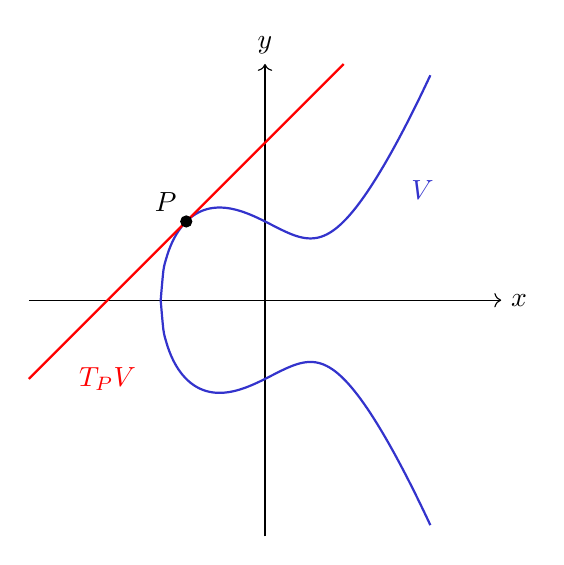
\begin{tikzpicture}
  % Draw axes
  \draw[->] (-3, 0) -- (3, 0) node[right] {$x$};
  \draw[->] (0, -3) -- (0, 3) node[above] {$y$};

  % Plot the curve y^2 = x^3 - x + 1 manually
  \draw[thick, blue, samples=100, smooth, domain=-1.32472:2.1, variable=\x] 
    plot ({\x}, {sqrt((\x)^3 - (\x) + 1)});
  \draw[thick, blue, samples=100, smooth, domain=-1.32472:2.1, variable=\x] 
    plot ({\x}, {-sqrt((\x)^3 - (\x) + 1)});

  % Tangent line y = (x + 1) + 1
  \draw[thick, red, domain=-3:1] plot(\x, {(\x+1)+1});

  % Mark the point (-1, 1)
  \filldraw[black] (-1, 1) circle (2pt) node[above left] {$P$};

  % Labels for the curve and tangent line
  \node[blue] at (2, 1.4) {$V$};
  \node[red] at (-2, -1) {$T_PV$};
\end{tikzpicture}
\caption{The tangent space of $V = \bV(y^2 - x^3 + x - 1)$ at $P=(-1, 1)$.}
\label{figure:tangentspace}
\end{figure}

Now let $V\subseteq\AA^n$ be any algebraic set.
Given $f\in\bI(V)$, we compute $f_P^{(1)}$ using Equation \ref{equationtangent}.
The tangent space of $V$ at $P$ is
$$T_PV := \bigcap_{f\in\bI(V)} \bV(f_P^{(1)}).$$
In other words, $T_PV$ is the intersection of all affine subspaces tangent at $P$ to some $f$ in the ideal $\bI(V)$ defining $V$.

We now explain how the intersection defining $T_PV$ may be replaced with a finite intersection.
Suppose $f_1, \ldots, f_m$ generate $\bI(V)$.
Then for any $f = \sum_{j=1}^m h_j f_j \in \bI(V)$ and $P \in V$, one readily computes that
\begin{align*}
	f_P^{(1)} &= \sum_{j=1}^m h_j(P) \sum_{i=1}^n \frac{\partial f_j}{\partial X_i}(P)(X_i-a_i).
\end{align*}
Thus $f_P^{(1)}$ is a linear combination of the polynomials $f_{j,P}^{(1)}$.
It follows that $f_P^{(1)}$ vanishes whenever all the $f_{j,P}^{(1)}$ do, so
$$\bigcap_{j=1}^m \bV(f_{j,P}^{(1)}) \subseteq \bigcap_{f \in \bI(V)} \bV(f_P^{(1)}).$$
The opposite inclusion is clear, and therefore
$$T_PV=\bigcap_{j=1}^m \bV(f_{j,P}^{(1)}).$$

We now explain why $T_PV$ is a vector space over $k$ and therefore has a dimension.
It is clear that that zero vector is the point $P$.
The addition and scalar multiplication is defined as follows: if $Q_1, Q_2 \in \AA^n$ lying in $T_PV$ are written $Q_i = \tilde Q_i + P$, then
$$Q_1 + Q_2 = (\tilde Q_1 + \tilde Q_2) + P, \qquad\qquad \lambda \cdot Q_i = \lambda \tilde Q_i + P, \,\,\, \lambda \in k.$$
This is the usual vector space structure on $k^n$ if the origin is translated to $P$.

We now define the dimension of the algebraic set $V$ by
$$\dim V := \min\{\dim T_PV : P \in V\}.$$
A point $P \in V$ is called non-singular if $\dim T_PV = \dim V$ and singular if $\dim T_P V > \dim V$.
We denote the set of non-singular and singular points by $V_{\text{non-sing}}$ and $V_{\text{sing}}$, respectively;
$V$ is called non-singular if it is non-singular at every point.

We now give examples computing tangent spaces and dimensions of algebraic sets.

\begin{example}
\begin{enumerate}
\item
Consider the trivial example $V = \AA^n$.
The ideal $\bI(V)$ is generated by $f = 1$, which for any $P$ has first-order part $f_P^{(1)} = 0$.
Then $T_PV = \bV(f_P^{(1)}) = \AA^n$, i.e., $T_PV$ is the vector space $k^n$ with the origin translated to $P$.
As expected, $\dim V = n$, and $\AA^n$ is non-singular.

\item
Consider $V = \bV(f) \subseteq \AA^2$, where $f = Y^2 - X^3 - 2X^2$.
For $P = (a, b)$, one computes
$$f_P^{(1)} = \frac{\partial f}{\partial X}(P)(X-a) + \frac{\partial f}{\partial Y}(P)(Y-b) = a(-3a-4)(X - a) + 2b(Y-b).$$ 
The tangent space $\bV(f_P^{(1)})$ is a line if at least one of the coefficients $a(-3a-4)$ and $2b$ does not vanish, and all of $\AA^2$ otherwise.
Of the points $(0, 0)$ and $(-\frac{4}{3}, 0)$ which make the coefficients vanish, only $(0, 0)$ lies in $V$.
Then $T_PV$ is a line for all points in $V\setminus\{(0, 0)\}$, and $T_{(0,0)}V = \AA^2$.
Thus, $\dim V = 1$ and $P = (0, 0)$ is a singular point of $V$.
\end{enumerate}
\end{example}

\begin{figure}[H]
     \begin{subfigure}[b]{0.49\textwidth}
          \centering
          \resizebox{\linewidth}{!}{
		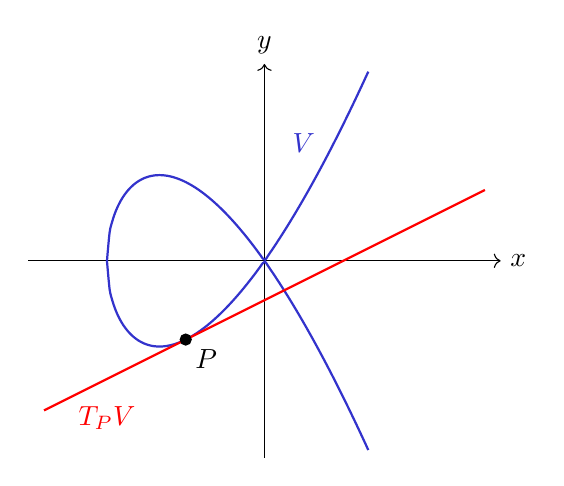
\begin{tikzpicture}
		  % Draw axes
		  \draw[->] (-3, 0) -- (3, 0) node[right] {$x$};
		  \draw[->] (0, -2.5) -- (0, 2.5) node[above] {$y$};
		
		  % Plot the curve y^2 = x^3 + 2x^2 manually
		  \draw[thick, blue, samples=100, smooth, domain=-2:1.32, variable=\x] 
		    plot ({\x}, {sqrt((\x)^3 + 2*(\x)^2)});
		  \draw[thick, blue, samples=100, smooth, domain=-2:1.32, variable=\x] 
		    plot ({\x}, {-sqrt((\x)^3 + 2*(\x)^2)});
		
		  % Tangent line y = 2 + (9/4)(X-1)
		  \draw[thick, red, domain=-2.8:2.8] plot(\x, {(1/2)*(\x+1)-1});
		
		  % Mark the point (-1, -1)
		  \filldraw[black] (-1, -1) circle (2pt) node[below right] {$P$};
		
		  % Labels for the curve and tangent line
		  \node[blue] at (0.5, 1.5) {$V$};
		  \node[red] at (-2, -2) {$T_PV$};
		\end{tikzpicture}
          }  
          \caption*{$P=(-1, -1)$}
          \label{fig:A}
     \end{subfigure}
     \begin{subfigure}[b]{0.49\textwidth}
          \centering
          \resizebox{\linewidth}{!}{
		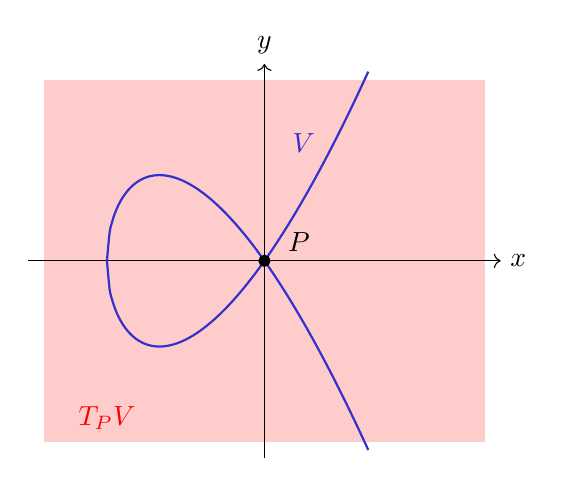
\begin{tikzpicture}
		  % Shading the background to represent T_PV being all of A^2
		  \fill[red!20] (-2.8, -2.3) rectangle (2.8, 2.3);
		
		  % Draw axes
		  \draw[->] (-3, 0) -- (3, 0) node[right] {$x$};
		  \draw[->] (0, -2.5) -- (0, 2.5) node[above] {$y$};
		
		  % Plot the curve y^2 = x^3 - x + 1 manually
		  \draw[thick, blue, samples=100, smooth, domain=-2:1.32, variable=\x] 
		    plot ({\x}, {sqrt((\x)^3 + 2*(\x)^2)});
		  \draw[thick, blue, samples=100, smooth, domain=-2:1.32, variable=\x] 
		    plot ({\x}, {-sqrt((\x)^3 + 2*(\x)^2)});
		
		  % Mark the point (0, 0)
		  \filldraw[black] (0, 0) circle (2pt) node[above right] {\,\,\,$P$};

		  % Labels for the curve and tangent line
		  \node[blue] at (0.5, 1.5) {$V$};
		  \node[red] at (-2, -2) {$T_PV$};
		\end{tikzpicture}
          }  
          \caption*{$P=(0,0)$}
          \label{fig:B}
     \end{subfigure}
     \caption{Two tangent spaces of $V = \bV(Y^2-X^3-2X^2)$.}
     \label{figure:}
\end{figure}

In the singular example above, $V_{\text{non-sing}}$ is the complement of a single point, in particular, it is an open subset of $V$.
This gives an example of the general fact that the set of non-singular points is an open subset of $V$.
To prove this fact, for an integer $r$ such that $0 \le r \le n$, define the subset
$$S(r) := \{P \in V : \dim T_P V \ge r\}\subseteq V.$$
If $d := \dim V$, then $V = S(d)$ and $V_{\text{sing}} = S(d+1)$.
Thus,
$$V_{\text{non-sing}} = V \setminus V_{\text{sing}} = V \setminus S(d+1).$$
To see $V_{\text{non-sing}}$ is open, it remains to show $S(d+1)$ is closed; this is the content of the following proposition:

\begin{proposition}[{\cite[\S 6.5]{Reid88}}]
The subset $S(r)$ is closed for all $r=0, \ldots, n$.
\end{proposition}
\begin{proof}
Let $f_1, \ldots, f_m$ generate $\bI(V)$.
From our previous discussion , we know $T_PV$ is the set of $(x_1, \ldots, x_n) \in \AA^n$ solving
$$\sum_{i=1}^n \frac{\partial f_j}{\partial X_i} (x_i - a_i) = 0$$
for all $j = 1, \ldots, m.$
Then $T_PV$ is identified with the kernel of the matrix 
$$J(P) := \left(\frac{\partial f_i}{\partial X_j}(P)\right)_{\substack{1 \le i \le m \\ 1 \le j \le n}}.$$
Checking $P$ lies in $S(r)$ is equivalent to checking $\rank (J(P)) \le n-r$.
In turn, this is equivalent to ensuring every $(n-r+1)\times(n-r+1)$ minor of $J(P)$ vanishes.
The entries of $J(P)$ are polynomials in $P=(a_1, \ldots, a_n)$.
Then each minor of $J(P)$ is also a polynomial, and so $S(r)$ is an algebraic set.
\end{proof}

Although the description we have given for $T_PV$ in terms of first-order parts of polynomials is geometrically intuitive, it depends on the embedding of $V$ into affine space.
We now prove a theorem which gives an intrinsic description of $T_PV$ in terms of ideals in the coordinate ring of $V$.

Suppose $V$ is an algebraic set in $\AA^n$ with $P \in V$.
Changing coordinates if necessary, we assume without loss of generality that $P=(0, \ldots, 0)$.
Now $T_PV$ is a vector subspace of $k^n$.
Write $\frakm_P\subseteq k[V]$ for the maximal ideal of regular functions vanishing at $P$, and denote by $M_P$ the ideal $(X_1, \ldots, X_n) \subseteq k[X_1,\ldots, X_n]$.
Note that we have $\frakm_P=M_P/\bI(V)$.
We are now ready to prove the theorem.

\begin{theorem}
There is a natural isomorphism of vector spaces
$$(T_PV)^* \cong \frakm_P/\frakm_P^2,$$
where $(T_PV)^*$ is the algebraic dual vector space of $T_PV$.
\end{theorem}
\begin{proof}
We first prove the special case $V=\AA^n$, where we must show $M_P/M_P^2\cong(k^n)^*$.
Note that $\{X_1, \ldots, X_n\}$ is a basis for $(k^n)^*$.
As $P=(0, \ldots, 0)$, the first-order part
$$f_P^{(1)}=\sum_{i=1}^n \frac{\partial f}{\partial X_i}(P) X_i$$
is a linear form on $k^n$.
This gives rise to the map $d : M_P\to(k^n)^*$ defined by $f \mapsto f_P^{(1)}$.
It suffices to show $d$ is surjective with kernel $M_P^2$.
Note $d$ is surjective since the images of $X_i$ form to a basis for $(k^n)^*$.
Next, a general $f \in M_P$ can be written
$$f=\sum_{i=1}^n c_i X_i + \text{higher order terms},$$
for some $c_i \in k$.
Since $P=(0,\ldots,0)$, the first-order part equals
$$f_P^{(1)} = \sum_{i=1}^n c_i X_i.$$
Therefore $f \in \ker d$ if and only if each $c_i$ equals zero.
This is equivalent to $f$ lying in $M_P^2$, as $M_P^2$ is generated by the monomials $X_i X_j$.

For the general case, we show $(T_PV)^*$ and $\frakm_P/\frakm_P^2$ are both isomorphic to
$$M_P/(M_P^2+\bI(V)).$$

We now show $(T_PV)^* \cong M_P/(M_P^2+\bI(V))$.
Observe that we have the surjective restriction map $(k^n)^* \to (T_PV)^*$.
Composing $d$ with this restriction map yields another map
$$D:M_P \to (k^n)^* \to (T_PV)^*,$$
which is clearly surjective.
To prove the desired isomorphism, it suffices to show $\ker D = M_P^2+\bI(V)$.
We give equivalent conditions for $f$ to lie in $\ker D$.
By definition of $D$, the map $f$ lies in $\ker D$ if and only if $f_P^{(1)} \big|_{T_PV} = 0$.
If $g_j \in \bI(V)$ denote generators for $\bI(V)$, we know $T_PV = \bigcap_j \bV(g_{j,P}^{(1)}).$
Then $f_P^{(1)} \big|_{T_PV}=0$ if and only if 
$$f_P^{(1)} = \sum_j a_j g_{j,P}^{(1)}$$
for some $a_j \in k$.
The above equality is equivalent to $f$ and $\sum_j a_j g_j$ only differing by quadratic terms.
In other words, it is equivalent to the inclusion
$$f - \sum_j a_j g_j \in M_P^2,$$
which is the same as the inclusion $f \in M_P^2 + \bI(V)$.

To see $\frakm_P/\frakm_P^2 \cong M_P/(M_P^2+\bI(V))$, we find a surjective homomorphism $\varphi : M_P \to \frakm_P/\frakm_P^2$ with kernel $M_P^2+\bI(V)$. 
To this end, define $\varphi$ by $h \mapsto (h+\bI(V)) + \frakm_P^2$.
This is well-defined and surjective since $\frakm_P=M_P/\bI(V)$.
Also,
$$\ker \varphi = \{h \in M_P : h + \bI(V) \in \frakm_P^2\}=\{h \in M_P:h+\bI(V)\in M_P^2/\bI(V)\}=M_P^2+\bI(V).$$
\end{proof}










\newpage
%\addtocontents{toc}{\vskip 1em}
\section{Convex geometry}\label{chapter:convexgeometry}
An affine toric variety is an affine variety defined using a cone in a vector space.
Many properties of the variety are determined by properties of the cone.
Thus, to study toric varieties, it is important to understand the convex geometry of cones.
The goal of this chapter is to study the convex geometry we will need to study toric varieties.

We begin by defining convex cones and providing examples.
Analogous to how vector spaces have dual spaces, cones have dual cones.
One of the main results we prove in this chapter is that dualising a convex cone twice yields the same cone---this is a fundamental fact, but the proof is non-trivial.
Studying cones is more subtle than studying vector spaces because cones are not linear objects.
For example, a cone may have different dimension to its dual (c.f.\ Example \ref{example:conesandduals}), unlike finite-dimensional vector spaces, where the dimension of the dual is the same.

In the context of toric varieties, the cones we are interested in have certain properties like being polyhedral, strongly convex, and rational.
An important part of this chapter is clearly defining these properties.
In Chapter \ref{affinetoricvarieties}, we will see how these properties have consequences for toric varieties.

%Since we are interested in applying convex geometry to the study of toric varieties, the reader is invited to skim this chapter on their first reading.
%Subsequent chapters should be readable with just a basic understanding of the definitions in this chapter.
%The reader can return to this chapter for the results herein as they are needed.





\subsection{Convex cones}\label{section:convexcones}
In this section, we define convex cones and their duals.
We also prove that dualising a cone twice yields the original cone.

Throughout this chapter, $N_\RR$ denotes a real vector space of finite dimension $n$, with algebraic dual space $M_\RR = N_\RR^*$.
We have the dual pairing $\langle \cdot, \cdot \rangle : M_\RR \times N_\RR \to \RR$ given by $\langle u, v \rangle := u(v)$.

A subset $\sigma \subseteq N_\RR$ is a cone if it is closed under non-negative scalar multiplication, i.e., $\lambda x \in \sigma$ for all $x \in \sigma$ and all $\lambda \in \RR_{\ge 0}$.
A set $\sigma \subseteq N_\RR$ is convex if for any two points in $\sigma$, the line segment joining them is contained in $\sigma$,
i.e., $x, y \in \sigma$ implies $\lambda x + (1 - \lambda) y \in \sigma$ for all $\lambda \in [0, 1]$.
Since cones are closed under positive scalar multiplication, a cone is convex if and only if it is closed under addition.

The dimension of a cone $\sigma$ is
$$\dim(\sigma) := \dim(\RR \cdot \sigma),$$
where $\RR\cdot\sigma = \sigma + (-\sigma)$ is the smallest vector subspace of $N_\RR$ containing $\sigma$.
We say $\sigma$ is non-degenerate if $\dim(\sigma) = \dim N_\RR$.

\begin{example}\label{example:cones}
\begin{enumerate}
\item
The two rays
$$\sigma_1 = \{(x, x), \, (x, 2x) : x \in \RR_{\ge 0}\}$$
is a cone but not convex.
We can ``fill in'' $\sigma_1$ to get the convex cone
$$\sigma_2 = \{(x, y) \in \RR_{\ge 0}^2 : x \le y \le 2 x\}.$$
We have $\dim (\sigma_1) = \dim(\sigma_2)=2$.

\item
An example of a convex cone in $\RR^3$ is
$$\sigma_3 = \{(x, r) \in \RR^2 \times \RR : \|x\| \le r\}.$$
We have $\dim(\sigma_3)=3$.
\end{enumerate}
\noindent
See Figure \ref{figure:cones} for plots of these cones.
\end{example}

\begin{figure}[h]
     \begin{subfigure}[b]{0.325\textwidth}
          \centering
          \resizebox{0.8 \linewidth}{!}{
              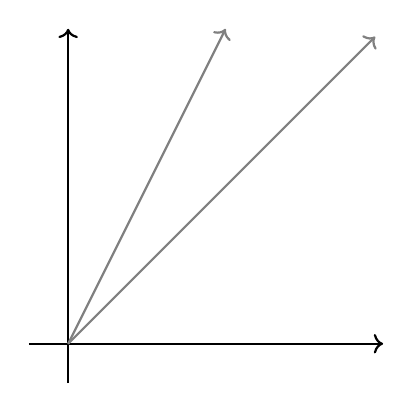
\begin{tikzpicture}
      		\draw[->,thick] (-0.5,0) -- (4,0);
      		\draw[->,thick] (0,-0.5) -- (0,4);
      		\draw[gray,thick,->,domain=0:3.9] plot (\x,\x);
      		\draw[gray,thick,->,domain=0:2] plot (\x,{2*\x});
    	    \end{tikzpicture}         
          }  
          \caption*{$\sigma_1$}
          \label{fig:A}
     \end{subfigure}
     \begin{subfigure}[b]{0.325\textwidth}
          \centering
          \resizebox{0.8 \linewidth}{!}{
              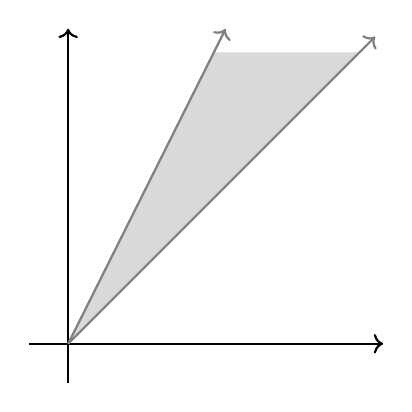
\begin{tikzpicture}
      		\draw[->,thick] (-0.5,0) -- (4,0);
      		\draw[->,thick] (0,-0.5) -- (0,4);
		    \fill[gray!30] (0,0) -- plot[domain=0:3.7] (\x,{\x}) -- plot[domain=1.85:0] (\x,{2*\x}) -- cycle;
      		\draw[gray,thick,->,domain=0:3.9] plot (\x,{\x});
      		\draw[gray,thick,->,domain=0:2] plot (\x,{2*\x});
    	\end{tikzpicture}          
          }  
          \caption*{$\sigma_2$}
          \label{fig:B}
     \end{subfigure}
     \begin{subfigure}[b]{0.325\textwidth}
          \centering
          \resizebox{\linewidth}{!}{
              \begin{tikzpicture}[tdplot_main_coords]
				\coordinate (O) at (0,0,1);
         		 \draw (0,0,-1) -- (O);
      			 \draw[->] (-5,0,1) -- (5,0,1) node[right] {};
     		 	 \draw[->] (0,-5,1) -- (0,5,1) node[right] {};
     		     \coneback[surface]{3}{2}{11}
     		     \draw[->] (O) -- (0,0,5) node[above] {};
      		     \conefront[surface]{3}{2}{13}
   	 \end{tikzpicture}
          }  
          \caption*{$\sigma_3$}
          \label{fig:C}
     \end{subfigure}
     \caption{The three cones in Example \ref{example:cones}.}
     \label{figure:cones}
\end{figure}

In linear algebra, dualising is an important operation which helps us to study a vector space.
In convex geometry, there is an similar notion for a cone, called the dual cone.
We will explore the relationship between a cone and its dual throughout this chapter.
We now give the definition:

\begin{definition}
Let $\sigma$ be a cone in $N_\RR$.
The dual cone $\sigma^\vee$ is
$$\sigma^\vee := \{u \in M_\RR : \langle u, v \rangle \ge 0 \text{ for all } v \in \sigma\}.$$
\end{definition}

We now give examples of cones and their duals.

\begin{example}\label{example:conesandduals}
Consider the vector space $N_\RR = \RR^n$.
Let $e_1, \ldots, e_n$ be the standard basis for $N_\RR$ and $e_1^*, \ldots, e_n^*$ the dual basis for $M_\RR$.
\begin{enumerate}
\item
Consider the cone $\sigma := \Span_{\RR_{\ge 0}}\{e_1, \ldots, e_n\}.$
Observe that a functional $\sum_{i=1}^n a_i e_i^*$ is in the dual cone if and only if $a_i \ge 0$ for all $i$.
Then $\sigma^\vee = \Span_{\RR_{\ge 0}}\{e_1^*, \ldots, e_n^*\}$.

\item
Now consider the cone $\sigma := \Span_{\RR_{\ge 0}}\{e_1^*, \ldots, e_r^*\}$, where $1 \le r \le n$.
The functional $\sum_{i=1}^n a_i e_i^*$ is in the dual cone if and only if $a_i \ge 0$ for all $1 \le i \le r$.
Thus, $\sigma^\vee = \Span_{\RR_{\ge 0}}\{e_1^*, \ldots, e_r^*, \pm e_{r+1}^*, \ldots, \pm e_n^*\}.$
Notice $\dim(\sigma)=r$ while $\dim(\sigma^\vee) = n$, showing $\sigma$ and $\sigma^\vee$ may have different dimensions.

\item
Let $n = 2$ and consider the cone $\sigma = \Span_{\RR_{\ge 0}} \{e_1, - e_1 + 2 e_2\}.$
To determine the elements $u\in\sigma^\vee$, we only need to check when $\langle u, v \rangle \ge 0$ for the generators $v = e_1$ and $v = -e_1 + 2 e_2$.
Then $u = a_1 e_1^* + a_2 e_2^* \in M_\RR$ lies in $\sigma^\vee$ precisely when the following two inequalities hold:
$$\langle u, e_1 \rangle = a_1 \ge 0, \quad \langle u, -e_1 + 2e_2 \rangle = -a_1 + 2a_2 \ge 0.$$
In view of Figure \ref{figureconeanddual}, we see  $\sigma^\vee = \Span_{\RR_{\ge 0}} \{2 e_1 + e_2, e_2\}.$
\end{enumerate}
\end{example}

\begin{figure}[H]
    \centering
    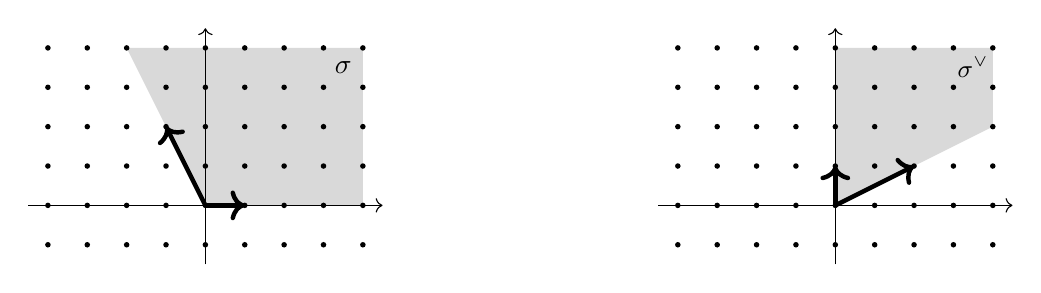
\begin{tikzpicture}
        % Left diagram
        \begin{scope}[shift={(-4,0)}]
            % Shaded area
            \fill[gray!30] (0,0) -- (-1,2) -- (2,2) -- (2,0) -- cycle;
            
            % Axes
            \draw[->] (-2.25,0) -- (2.25,0);
            \draw[->] (0,-0.75) -- (0,2.25);
            
            % Lattice points
            \foreach \x in {-2,-1.5,-1,-0.5,0,0.5,1,1.5,2}
                \foreach \y in {-0.5,0,0.5,1,1.5,2}
                    \fill (\x,\y) circle (1pt);

            % Vectors
            \draw[->, ultra thick] (0,0) -- (0.5,0);
            \draw[->, ultra thick] (0,0) -- (-0.5,1);
            \node at (1.75, 1.75) {$\sigma$};
        \end{scope}
        
        % Right diagram
        \begin{scope}[shift={(4,0)}]
            % Shaded area
            \fill[gray!30] (0,0) -- (0,2) -- (2,2) -- (2, 1) -- cycle;
            
            % Axes
            \draw[->] (-2.25,0) -- (2.25,0);
            \draw[->] (0,-0.75) -- (0,2.25);
            
            % Lattice points
            \foreach \x in {-2,-1.5,-1,-0.5,0,0.5,1,1.5,2}
                \foreach \y in {-0.5,0,0.5,1,1.5,2}
                    \fill (\x,\y) circle (1pt);

            % Vectors
            \draw[->, ultra thick] (0,0) -- (0,0.5);
            \draw[->, ultra thick] (0,0) -- (1,0.5);
            \node at (1.75, 1.75) {\small{$\sigma^\vee$}};
        \end{scope}
    \end{tikzpicture}
    \caption{The cone $\sigma=\Span_{\RR_{\ge 0}} \{e_1, - e_1 + 2 e_2\}$ and its dual.}
     \label{figureconeanddual}
\end{figure}

The following theorem relates a cone to its dual and has many important consequences;
for example, it is not obvious that dualising a cone twice yields the original cone, but the theorem establishes this fact (c.f.\ Corollary \ref{corollary:doubledual}).
We need to define a topology on $N_\RR$ to state the theorem.
Choose any vector space isomorphism $N_\RR \to \RR^n$, and define the topology on $N_\RR$ by declaring this map to also be a homeomorphism.
Since linear transformations $\RR^n \to \RR^n$ are continuous, the topology we have defined doesn't depend on the choice of isomorphism.

\begin{theorem}[{\cite[\S 1.2]{Fulton93}}]\label{theorem:dualcone}
Let $\sigma$ be a topologically closed convex cone in $N_\RR$.
If $v \notin \sigma$, then there exists $u \in \sigma^\vee$ such that $\langle u, v \rangle <0.$
\end{theorem}

References such as \cite{Fulton93}, \cite{CLS11}, and \cite{Oda88} omit a proof of Theorem \ref{theorem:dualcone}, but we present one, following \cite{BV04}.
We begin with a lemma from analysis:

\begin{lemma}\label{lemma:mindistance}
Let $A$ and $B$ be disjoint, topologically closed subsets of a Euclidean vector space $(V, (\cdot,\cdot))$, and assume $A$ is compact.
Then there exist $a_{\text{min}} \in A$ and $b_{\text{min}} \in B$ which minimise the distance $\|a-b\|$ over all $a \in A$ and $b \in B$.
(Here $\|\cdot\|$ is the norm induced by $(\cdot,\cdot)$.)
\end{lemma}
%%%% THIS IS A WIKIPEDIA PROOF; FIND A REFERENCE %%%
\begin{proof}
Take arbitrary $x \in A$ and $y \in B$ and set $r_1 := \|x-y\| > 0$.
Since $A$ is compact, it is bounded by a closed ball of some radius $r_2 > 0$.
Let $S := B \cap \overline{B_{r_1+r_2}(x)},$ which is non-empty since $y \in S$.
Since the distance function is continuous and $A \times S$ is compact, there exists $(a_{\text{min}}, b_{\text{min}}) \in A \times S$ minimising the distance $\|a - b\|$ for all pairs of points in $A \times S$.
We claim that this is in fact the minimum for all pairs of points in $A \times B$.
Suppose to the contrary that there is $(\alpha,\beta) \in A \times B$ with $\|\alpha - \beta\| < \|a_{\text{min}} - b_{\text{min}}\|$. 
In particular, since $\|a_{\text{min}} - b_{\text{min}}\|\le r_1$, $\|\alpha - \beta\| < r_1$ and so
$\|x - \beta\| \le \|x- \alpha\| + \|\alpha - \beta\| < r_2 + r_1.$
This implies $\beta$ lies in $S$, contradicting that $\|a_{\text{min}} - b_{\text{min}}\|$ attained the minimum distance for pairs in $A \times S$.
\end{proof}

The proof of Theorem \ref{theorem:dualcone} follows from the following hyperplane separation theorem, which says that for certain sets, we can find a hyperplane so that each set lies in a different half-space.

\begin{theorem}[Hyperplane separation theorem {\cite[\S 2.5.1]{BV04}}]\label{hyperplaneseparation}
Under the assumptions of Lemma \ref{lemma:mindistance}, there exists $w \in V\setminus\{0\}$ and $\lambda \in \RR$ such that for all $a \in A$, $(w, a) \le \lambda$, and for all $b \in B$, $(w, b) \ge \lambda$.
\end{theorem}

\begin{proof}
Lemma \ref{lemma:mindistance} yields $a_{\text{min}} \in A$ and $b_{\text{min}} \in B$ minimising the distance between points in $A$ and points in $B$.
Then the desired $w$ and $\lambda$ are
$$w := b_{\text{min}} - a_{\text{min}}, \qquad\text{and}\qquad \lambda := \frac{1}{2}(b_{\text{min}} - a_{\text{min}}, b_{\text{min}} + a_{\text{min}}).$$
The hyperplane defined by $(w, \cdot) = \lambda$ is orthogonal to the line segment joining $a_{\text{min}}$ and $b_{\text{min}}$ and passes through the midpoint.
Let us prove that $(w, b) \ge \lambda$ for all $b \in B$ (a similar argument shows $(w, a) \le \lambda$ for all $a \in A$).
Proceeding by contradiction, assume that there exists $u \in B$ with $(w, u) < \lambda$.
Then by definition of $w$ and $\lambda$, this means 
$$0 > (w, u) -\frac{1}{2}(w, b_{\text{min}}+a_{\text{min}}) = (w, u-b_{\text{min}}+\frac{1}{2} (b_{\text{min}}-a_{\text{min}})) =(w, u-b_{\text{min}})+\frac{1}{2}\|w\|^2,$$
so in particular, $(w, u-b_{\text{min}})<0$.
Consider the function
$$g(t):=\|w+t(u-b_{\text{min}})\|^2.$$
Note that $g(0)=\|w\|$, and using the Leibniz rule for differentiating inner products, we see
$$g'(0) = 2 (w+t(u-b_{\text{min}}), u-b_{\text{min}}) \big|_{t=0} = 2 (w, u-b_{\text{min}}) < 0.$$
This implies that for small $t > 0$, $g(0) > g(t)$.
In other words,
$$\|b_{\text{min}} - a_{\text{min}}\| > \|b_{\text{min}} + t(u - b_{\text{min}}) - a_{\text{min}}\|.$$
But $B$ is convex and contains $b_{\text{min}}$ and $u$, so $B$ also contains $(b_{\text{min}} + t (u - b_{\text{min}}))$.
This contradicts the minimality of $\|b_{\text{min}} - a_{\text{min}}\|$.
\end{proof}

To prove Theorem \ref{theorem:dualcone}, we use the hyperplane separation theorem to find a certain hyperplane containing zero, which gives rise to the desired functional $u\in\sigma^\vee$.

\begin{proof}[Proof of Theorem \ref{theorem:dualcone} \textup{(\cite[Example 2.20]{BV04})}]
Fix a basis $e_1, \ldots, e_n$ for $N_\RR$ and endow $N_\RR$ with the inner product which makes the basis orthonormal.
Since $\sigma$ is topologically closed and $v \notin \sigma$, there exists $\varepsilon > 0$ such that $\overline{B_\varepsilon(v)}$ does not intersect $\sigma$.
By Theorem \ref{hyperplaneseparation}, there exist $w \in N_\RR$ and $\lambda \in \RR$ such that $(w, x) \ge \lambda$ for all $x \in \sigma$ and $(w, y) \le \lambda$ for all $y \in \overline{B_\varepsilon(v)}$.
In fact, we must have $\lambda \le 0$ since $0$ lies in $\sigma$.

We claim that $(w, x) \ge 0$ for all $x \in \sigma$ and $(w, v) < 0$.
This completes the proof, as then $u$ defined by $x \mapsto (w, x)$ is a linear form in $\sigma^\vee$ with $\langle u, v \rangle < 0$.
To see the first claim, suppose there exists $x \in \sigma$ with $(w, x) =: \lambda' < 0$.
Then for any $s \in \RR_{\ge 0}$, $s x \in \sigma $ and $(w, s x) = s \lambda'$, contradicting that $\{(w, x) : x \in \sigma\}$ is bounded from below.
To see the second claim, we just need to show $(w, v) \ne 0$.
Suppose we had $(w, v) = 0$.
As $y := v + \frac{\varepsilon w}{\|w\|}$ lies in $\overline{B_\varepsilon(v)}$, we get
$$\lambda \ge (w, y) = (w, v + \varepsilon w/\|w\|) = \varepsilon \|w\| > 0,$$
contradicting that $\lambda \le 0$.
\end{proof}

\begin{corollary}\label{corollary:doubledual}
Let $\sigma$ be a topologically closed cone in $N_\RR$.
Then $(\sigma^\vee)^\vee = \sigma$.
\end{corollary}
\begin{proof}
If $v \in \sigma$, then $\langle u, v\rangle \ge 0$ for all $u \in \sigma^\vee$, so $v \in (\sigma^\vee)^\vee$.
If $v \notin \sigma$, then Theorem \ref{theorem:dualcone} implies there exists $u \in \sigma^\vee$ with $\langle u, v \rangle < 0$ so that $v \notin (\sigma^\vee)^\vee$.
\end{proof}





\subsection{Polyhedral cones}\label{polyhedralcones}
In this section, we define a class of convex cones called polyhedral cones---these are cones with a finite set of generators.
The cones associated to toric varieties are always polyhedral.
We also define and study faces of polyhedral cones, which are important subsets of the cone.

\begin{definition}\label{definition:convexpolyhedral}
A subset $\sigma$ of $N_\RR$ is called a (convex) polyhedral cone if
$$\sigma = \Span_{\RR_{\ge 0}} \{v_1, \ldots, v_r\}$$
for a finite set of generators $v_1, \ldots, v_r \in N_\RR$.
\end{definition}

It follows from the definition that convex polyhedral cones are indeed convex cones in the sense defined in \S \ref{section:convexcones}.
Every example of convex cones we have seen so far has been polyhedral, except for $\sigma_3 = \{(x, r) \in \RR^2 \times \RR : \|x\| \le r\}$ in Example \ref{example:cones}.
%Recall that the dual cone $\sigma^\vee$ is the set of functionals which are non-negative on $\sigma$.
%When $\sigma$ is polyhedral, a functional lies in $\sigma^\vee$ if and only if it is non-negative on the generators of $\sigma$.

One definition of a convex polyhedron is a finite intersection of closed half-spaces in $\RR^3$.
The name polyhedral is justified by the following result:

\begin{theorem}
A cone satisfies Definition \ref{definition:convexpolyhedral} if and only if it is a finite intersection of closed half-spaces.
\end{theorem}
\begin{proof}
Later, in Proposition \ref{proposition:dualdescription}, we give a dual description of polyhedral cones, showing they are finite intersections of closed half-spaces.
The converse is proven in \cite[1.3.13]{DLHK13}.
\end{proof}

We now define the faces of a polyhedral cone.
Any $u \in M_\RR$ defines a subspace of $N_\RR$ in the following manner:
$$u^\perp = \{v \in N_\RR : \langle u, v \rangle = 0\}.$$
When $u$ is non-zero, $\dim u^\perp = n -1$.
The notation suggests we can intuitively think of $u^\perp$ as the orthogonal complement of $u$, though this interpretation is not strictly accurate since $\langle \cdot, \cdot \rangle$ is not an inner product.
A face $\tau$ of $\sigma$ is a set of the form 
$$\tau = \sigma \cap u^\perp,$$
for some $u \in \sigma^\vee$.
In other words, a face is the intersection of $\sigma$ with a hyperplane, such that $\sigma$ lies in the positive half-space of the hyperplane.
When $u = 0$, we have $\sigma \cap u^\perp = \sigma$, so $\sigma$ is a face of itself.
A face of codimension 1 is called a facet.
Let us give a basic example to illustrate these definitions.

\begin{example}
Consider $\sigma = \Span_{\RR_{\ge 0}} \{e_1, e_2\}$ in $N_\RR = \RR^2$.
We saw in Example \ref{example:conesandduals} that $\sigma^\vee = \Span_{\RR_{\ge 0}}\{e_1^*, e_2^*\}$.
Suppose $u = b_1 e_1^* + b_2 e_2^*$ lies in $\sigma^\vee$.
If $b_1$ and $b_2$ are both non-zero, then
$$\sigma \cap u^\perp = \{(a_1, a_2) \in \RR_{\ge 0}^2 : a_1 b_1 + a_2 b_2 = 0\} = \{0\}.$$
If $b_1 \ne 0$ but $b_2 = 0$, then
$$\sigma \cap u^\perp = \{(a_1, a_2) \in \RR_{\ge 0}^2 : a_1 b_1 = 0\} = \Span_{\RR_{\ge 0}}\{e_2\}.$$
Similarly, if $b_1 = 0$ but $b_2 \ne 0$, then $\sigma \cap u^\perp = \Span_{\RR_{\ge 0}} \{e_1\}.$
Figure \ref{figure:facesandnormals} shows the faces of $\sigma$ and functionals which define the faces.
\end{example}

%\begin{figure}[H]
%    \centering
%    \begin{tikzpicture}
%        % Left diagram
%        \begin{scope}[shift={(-3,0)}]
%            % Shaded area
%            \fill[gray!30] (0,0) -- (0,2) -- (2,2) -- (2,0) -- cycle;
%            
%            % Axes
%            \draw[-] (-.75,0) -- (2.25,0);
%            \draw[-] (0,-0.75) -- (0,2.25);
%            
%            % Lattice points
%            \foreach \x in {0.5,1,1.5,2}
%                \foreach \y in {0.5,1,1.5,2}
%                    \fill (\x,\y) circle (1pt);
%
%            % Vectors
%            \draw[->, ultra thick, red] (0,0) -- (0,2.25);
%            \draw[->, ultra thick, blue] (0,0) -- (2.25,0);
%	  \filldraw[black] (0, 0) circle (2.5pt);
%
%	   % Labels
%            \node at (1.5, 2.5) {\small{$\sigma = \sigma \cap 0^\perp$}};
%            \node[red] at (-1.25, 1.5) {\small{$\tau_2 = \sigma \cap u_2^\perp$}};
%            \node[blue] at (1.5, -0.5) {\small{$\tau_3 = \sigma \cap u_3^\perp$}};
%            \node at (-1.25, -0.5) {\small{$\tau_1 = \sigma \cap u_1^\perp$}};
%        \end{scope}
%        
%        % Right diagram
%        \begin{scope}[shift={(4,0)}]
%            % Shaded area
%            \fill[gray!30] (0,0) -- (0,2) -- (2,2) -- (2, 0) -- cycle;
%            
%            % Axes
%            \draw[->] (-.75,0) -- (2.25,0);
%            \draw[->] (0,-0.75) -- (0,2.25);
%            
%            % Lattice points
%            \foreach \x in {0,0.5,1,1.5,2}
%                \foreach \y in {0,0.5,1,1.5,2}
%                    \fill (\x,\y) circle (1pt);
%
%            % Vectors
%            \draw[->, ultra thick, blue] (0,0) -- (0,0.5);
%            \draw[->, ultra thick] (0,0) -- (0.5,0.5);
%	   \draw[->, ultra thick, red] (0,0) -- (0.5,0);
%            \node at (1.5, 2.5) {\small{$\sigma^\vee$}};
%
%	   % Labels
%            \node[red, below right] at (0.5,0) {\small{$u_2$}};
%            \node[blue, above left] at (0, 0.5) {\small{$u_3$}};
%            \node[above right] at (0.5, 0.5) {\small{$u_1$}};
%        \end{scope}
%    \end{tikzpicture}
%    \caption{}
%     \label{}
%\end{figure}

\begin{figure}[H]
    \centering
    % Left subfigure
    \begin{subfigure}[b]{0.45\textwidth}
        \centering
        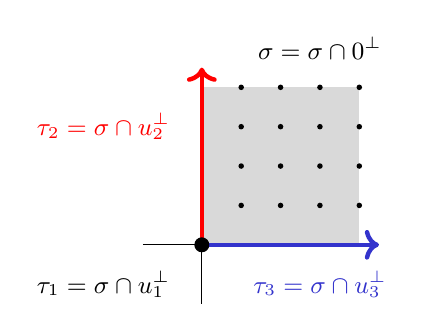
\begin{tikzpicture}
            % Shaded area
            \fill[gray!30] (0,0) -- (0,2) -- (2,2) -- (2,0) -- cycle;
            
            % Axes
            \draw[-] (-.75,0) -- (2.25,0);
            \draw[-] (0,-0.75) -- (0,2.25);
            
            % Lattice points
            \foreach \x in {0.5,1,1.5,2}
                \foreach \y in {0.5,1,1.5,2}
                    \fill (\x,\y) circle (1pt);

            % Vectors
            \draw[->, ultra thick, red] (0,0) -- (0,2.25);
            \draw[->, ultra thick, blue] (0,0) -- (2.25,0);
            \filldraw[black] (0, 0) circle (2.5pt);

            % Labels
            \node at (1.5, 2.5) {\small{$\sigma = \sigma \cap 0^\perp$}};
            \node[red] at (-1.25, 1.5) {\small{$\tau_2 = \sigma \cap u_2^\perp$}};
            \node[blue] at (1.5, -0.5) {\small{$\tau_3 = \sigma \cap u_3^\perp$}};
            \node at (-1.25, -0.5) {\small{$\tau_1 = \sigma \cap u_1^\perp$}};
        \end{tikzpicture}
        %\caption{Left diagram}
        %\label{fig:left_diagram}
    \end{subfigure}
    \hspace{-0.05\textwidth} % Creates equal spacing between the subfigures
    % Right subfigure
    \begin{subfigure}[b]{0.45\textwidth}
        \centering
        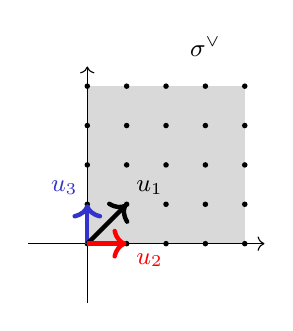
\begin{tikzpicture}
            % Shaded area
            \fill[gray!30] (0,0) -- (0,2) -- (2,2) -- (2, 0) -- cycle;
            
            % Axes
            \draw[->] (-.75,0) -- (2.25,0);
            \draw[->] (0,-0.75) -- (0,2.25);
            
            % Lattice points
            \foreach \x in {0,0.5,1,1.5,2}
                \foreach \y in {0,0.5,1,1.5,2}
                    \fill (\x,\y) circle (1pt);

            % Vectors
            \draw[->, ultra thick, blue] (0,0) -- (0,0.5);
            \draw[->, ultra thick] (0,0) -- (0.5,0.5);
            \draw[->, ultra thick, red] (0,0) -- (0.5,0);
            \node at (1.5, 2.5) {\small{$\sigma^\vee$}};

            % Labels
            \node[red, below right] at (0.5,0) {\small{$u_2$}};
            \node[blue, above left] at (0, 0.5) {\small{$u_3$}};
            \node[above right] at (0.5, 0.5) {\small{$u_1$}};
        \end{tikzpicture}
        %\caption{Right diagram}
        %\label{fig:right_diagram}
    \end{subfigure}
    \caption{The faces of $\sigma = \Span_{\RR_{\ge 0}}\{e_1, e_2\}$ and functionals defining them.}
    \label{figure:facesandnormals}
\end{figure}

We collect some basic properties of faces in the following proposition.

\begin{proposition}
Let $\sigma$ be a convex polyhedral cone.
\begin{enumerate}
\item A face of $\sigma$ is also a convex polyhedral cone.
\item There are only finitely many faces of $\sigma$.
\item Any intersection of faces is a face.
\item If $\tau$ is a face of $\sigma$, then a face of $\tau$ is also a face of $\sigma$.
\item Any proper face is contained in a facet.
Any proper face is the intersection of all the facets containing it, and a face with codimension two is the intersection of exactly two facets.
\end{enumerate}
\end{proposition}
\begin{proof}
See \cite[\S 1.2]{Fulton93} or \cite[\S 1]{Zaman13}.
\end{proof}





\subsection{Dual description of cones}\label{section:dualdescription}
We have seen some basic objects of convex geometry---cones and their duals---as well as some properties cones may have, like being polyhedral.
It is natural to ask whether the dual of a polyhedral cone is also polyhedral.
It turns out that this is the case, and this is the main result of this section:

\begin{theorem}[{Farkas's Lemma \cite[\S 1.2]{Fulton93}}]\label{theorem:farkas}
The dual of a convex polyhedral cone is a convex polyhedral cone.
\end{theorem}

The proof relies on giving a dual description of a polyhedral cone as an intersection of closed half-spaces.
To prepare for this, we discuss some basic topology of polyhedral cones.

Recall the interior of a subset $S$ of a topological space is the set of points admitting an open neighbourhood contained in $S$.
The boundary of $S$ is the set of points in the closure of $S$ which do not lie in the interior.
The following proposition characterises the boundary of a non-degenerate polyhedral cone:

\begin{proposition}\label{proposition:boundary}
The boundary of a non-degenerate polyhedral cone is the union of its proper faces.
\end{proposition}
\begin{proof}
See \cite[\S 1.2]{Fulton93} or \cite[\S 1]{Zaman13}.
\end{proof}

%When $\sigma$ is a cone which does not span $N_\RR$ (i.e., it is degenerate), its interior will be empty.
%For example, consider $\sigma = \Span_{\RR_{\ge 0}}\{e_1\}$ in $N_\RR = \RR^2$.
%Any open neighbourhood of a point in $\sigma$ contains a point outside $\sigma$, so its interior is empty.
%The fact that degenerate cones have empty interiors motivates the definition of the relative interior.
%The relative interior of $\sigma$ is defined as the interior of $\sigma$ in the vector space $\RR \cdot \sigma$.
%For example, when $\sigma = \Span_{\RR_{\ge 0}}\{e_1\}$, the relative interior of $\sigma$ is $\sigma \setminus\{0\}$.
%The following proposition characterises when a vector lies in the relative interior of a cone:
%
%\begin{proposition}
%Suppose that $\sigma$ is a polyhedral cone and $v \in \sigma$.
%The following are equivalent:
%\begin{enumerate}
%\item $v$ is in the relative interior of $\sigma$.
%\item $\langle u, v\rangle > 0$ for all $u \in \sigma^\vee \setminus \sigma^\perp.$
%\item $\sigma^\vee \cap v^\perp = \sigma^\perp$.
%\end{enumerate}
%\end{proposition}
%\begin{proof}
%See \cite[\S 1.2]{Fulton93} and \cite[\S 1]{Zaman13}.
%\end{proof}

We are ready to describe a polyhedral cone as an intersection of closed half-spaces.
We will need the following observation:
if $\sigma$ is non-degenerate and $\tau$ is a facet, then the functional $u_\tau \in \sigma^\vee$ such that $\tau = \sigma \cap u_\tau^\perp$ is unique up to positive scalar multiplication.
Indeed, any two such $u_\tau$ both vanish on the $(n-1)$-dimensional subspace $\RR \cdot \tau$, and their values on a point outside this subspace determine them, but these only differ by a positive scalar.
We now prove the result:

\begin{proposition}[{\cite[\S 1.2]{Fulton93}}]\label{proposition:dualdescription}
Let $\sigma$ be a non-degenerate cone in $N_\RR$ such that $\sigma \ne N_\RR$.
Then, $\sigma$ equals the intersection of half-spaces
$$H_\tau = \{v \in N_\RR : \langle u_\tau, v\rangle \ge 0\},$$
as $\tau$ ranges over the facets of $\sigma$.
\end{proposition}
\begin{proof}
The half-space $H_\tau$ does not depend on the choice of $u_\tau \in \sigma^\vee$ such that $\tau = \sigma \cap u_\tau^\perp$, since the functional $u_\tau$ is unique up to positive scalar multiplication.

If $v$ lies in $\sigma$, then $\langle u_\tau, v \rangle \ge 0$ for any facet $\tau$, since $u_\tau \in \sigma^\vee$.
Then $v$ lies in the intersection of half-spaces.

Conversely, suppose for the sake of contradiction that $v'$ is in the intersection of half-spaces but not in $\sigma$.
Since $\sigma$ is non-degenerate, Proposition \ref{proposition:boundary} implies there exists $v$ in the interior of $\sigma$.
There is a point $w$ on the line segment joining $v$ and $v'$ which also lies on the boundary of $\sigma$.
By Proposition \ref{proposition:boundary}, $w$ lies on a facet, say $\tau$.
Since $\langle u_\tau, v \rangle > 0$ and $\langle u_\tau, w \rangle = 0$, we have $\langle u_\tau, v' \rangle < 0$.
This contradicts that $v'$ lies in the intersection of the half-spaces.
\end{proof}

Proposition \ref{proposition:dualdescription} allows us to prove that the dual of a polyhedral cone is a polyhedral cone:

\begin{proof}[Proof of Theorem \ref{theorem:farkas}]
Suppose first that $\sigma$ is non-degenerate.
We show the $u_\tau$, where $\tau$ runs over the facets of $\sigma$, generate $\sigma^\vee$.
Suppose for the sake of contradiction there is $u \in \sigma^\vee$ which does not lie in the cone generated by the $u_\tau$.
Applying Theorem \ref{theorem:dualcone} to the cone generated by the $u_\tau$ tells us there exists $v \in N_\RR$ such that $\langle u_\tau, v\rangle \ge 0$ for all $\tau$, but $\langle u, v \rangle < 0$.
By Proposition \ref{proposition:dualdescription}, $v$ lies in $\sigma$, so $\langle u, v \rangle < 0$ contradicts that $u$ lies in $\sigma^\vee$.

Now suppose $\sigma$ spans $V$, a subspace strictly smaller than $N_\RR$.
Let $\tilde \sigma$ denote the cone $\sigma$ thought of as a cone in $V = \RR \cdot \sigma$.
Then $\tilde \sigma$ is non-degenerate so that $\tilde \sigma^\vee$ is a convex polyhedral cone in $V^* = N_\RR / V^\perp$.
Then $\sigma^\vee$ will be generated by lifts of generators of $\tilde \sigma^\vee$, along with vectors $u$ and $-u$, as $u$ ranges over a basis for $V^\perp$.
\end{proof}

Given generators for a polyhedral cone $\sigma$, it would be nice to find generators for the dual cone.
The proof we just saw tells us it is sufficient to find the functional $u_\tau$ for each facet $\tau$.

We describe an algorithm for finding the functionals $u_\tau$ when $\sigma$ is non-degenerate.
For each set of $n-1$ $\RR$-independent vectors in the generating set of $\sigma$, solve for $u \in M_\RR$ vanishing on them.
If $u$ changes sign on the rest of the generators, it does not lie in $\sigma^\vee$ and may be discarded.
Now suppose that one of $u$ and $-u$ is non-negative on the rest of the generators; without loss of generality we assume $u$ is.
In this case, $u$ lies in $\sigma^\vee$, the $n-1$ vectors generate a face $\tau$, and $u = u_\tau$ is the equation of the face.
%We then take $u$ as one of the generators of $\sigma^\vee$.

Let us consider an example of applying this algorithm.

\begin{example}\label{example:3dconeanddual}
Let $N = \ZZ^3$ and $N_\RR = \RR^3$.
Consider $\sigma := \Span_{\RR_{\ge 0}}\{ e_1, e_2, e_1+e_3, e_2 + e_3\}$.
Observe that $e_1^*$ vanishes on $e_2$ and $e_2+e_3$, and is non-negative on all generators of $\sigma$.
Similarly, $e_1^*+e_2^*-e_3^*$ vanishes on $e_1+e_3$ and $e_2+e_3$ and is non-negative on $\sigma$.
Continuing the algorithm for finding the functionals $u_\tau$ which define facets, we see they are
$$u_{\tau_1} = e_1^*, \qquad u_{\tau_2} = e_2^*, \qquad u_{\tau_3} = e_3^*, \qquad u_{\tau_4} = e_1^* + e_2^* - e_3^*.$$
%For each $u_{\tau_i}$, there is the corresponding facet $\tau_i = \sigma \cap u_{\tau_i}^\perp$.
%These are:
%\begin{align*}
%	&\tau_1 = \Span_{\RR_{\ge 0}}\{e_2, e_2+e_3\}, & &\tau_2 = \Span_{\RR_{\ge 0}} \{e_1, e_1+e_3\}, \\
%	&\tau_3 = \Span_{\RR_{\ge 0}}\{e_1, e_2\},  & &\tau_4 = \Span_{\RR_{\ge 0}} \{e_1+e_3, e_2+e_3\}.
%\end{align*}
%The other faces in $\sigma$ are the rays 
%\begin{align*}
%	&\tau_1 \cap \tau_3 = \Span_{\RR_{\ge 0}}\{e_2\}, & &\tau_1 \cap \tau_4 = \Span_{\RR_{\ge 0}} \{e_2+e_3\}, \\
%	&\tau_2 \cap \tau_3 = \Span_{\RR_{\ge 0}}\{e_1\}, & &\tau_2 \cap \tau_4 = \Span_{\RR_{\ge 0}} \{e_1+e_3\},
%\end{align*}
%and the origin $\bigcap_{i=1}^4 \tau_i = \{0\}.$
The dual cone is generated by $u_{\tau_1}, \ldots, u_{\tau_4}$, so
$$\sigma^\vee = \Span_{\RR_{\ge 0}} \{e_1^*, e_2^*, e_3^*, e_1^* +e_2^* - e_3^*\}.$$
%Figure \ref{figure:3dcone} contains a diagram of $\sigma$.
\begin{figure}[h]
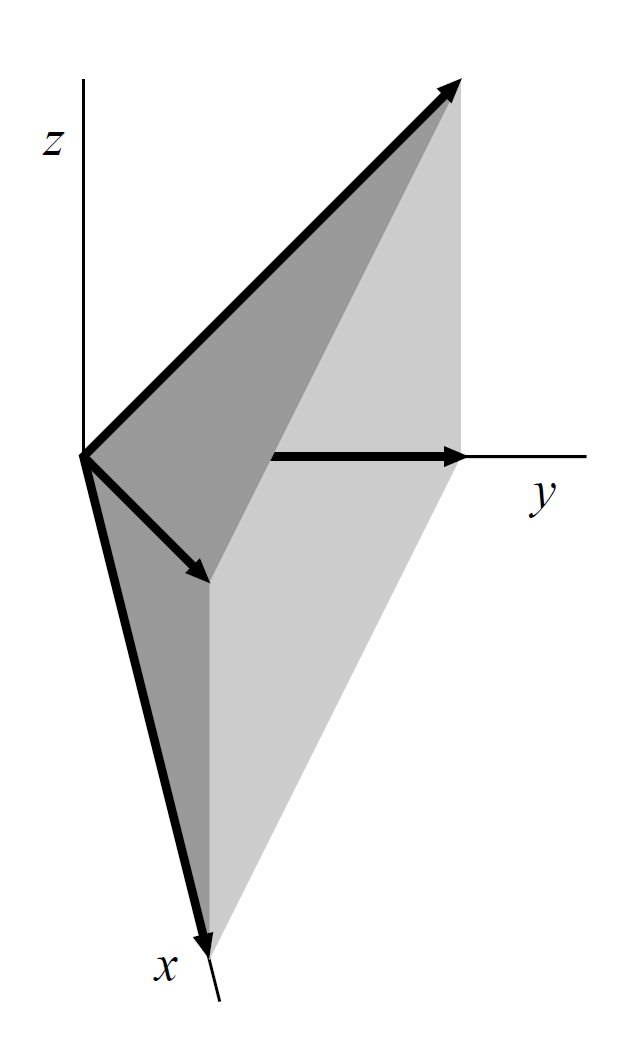
\includegraphics[width=0.2 \textwidth]{../images/cox cone example 2}
\caption{The cone $\sigma= \Span_{\RR_{\ge 0}}\{ e_1, e_2, e_1+e_3, e_2 + e_3\}$ \cite[Figure 2]{CLS11}.}
\label{figure:3dcone}
\end{figure}
\end{example}



\subsection{Strongly convex cones}
In this section, we define a class of polyhedral cones called strongly convex cones.
The cones used to study toric varieties are strongly convex.
We prove a useful proposition giving equivalent conditions for a cone to be strongly convex.
This involves a lemma providing a bijection between the faces of a cone and the faces of its dual.

We say a convex polyhedral cone is strongly convex if the origin of $N_\RR$ is a face.
Most of the cones we have seen in this chapter have been strongly convex.
An example of a polyhedral cone which is not strongly convex is the upper half-plane $\sigma = \Span_{\RR_{\ge 0}}\{e_1, -e_1, e_2\}$ in $N_\RR=\RR^2$.
The dual cone $\sigma^\vee$ is generated by $e_2^*$ and the only proper face is the $x$-axis.
Figure \ref{figure:strongconvexity} contains diagrams of two more cones: one which is strongly convex, and one which is not.

\begin{figure}[h]
\centering
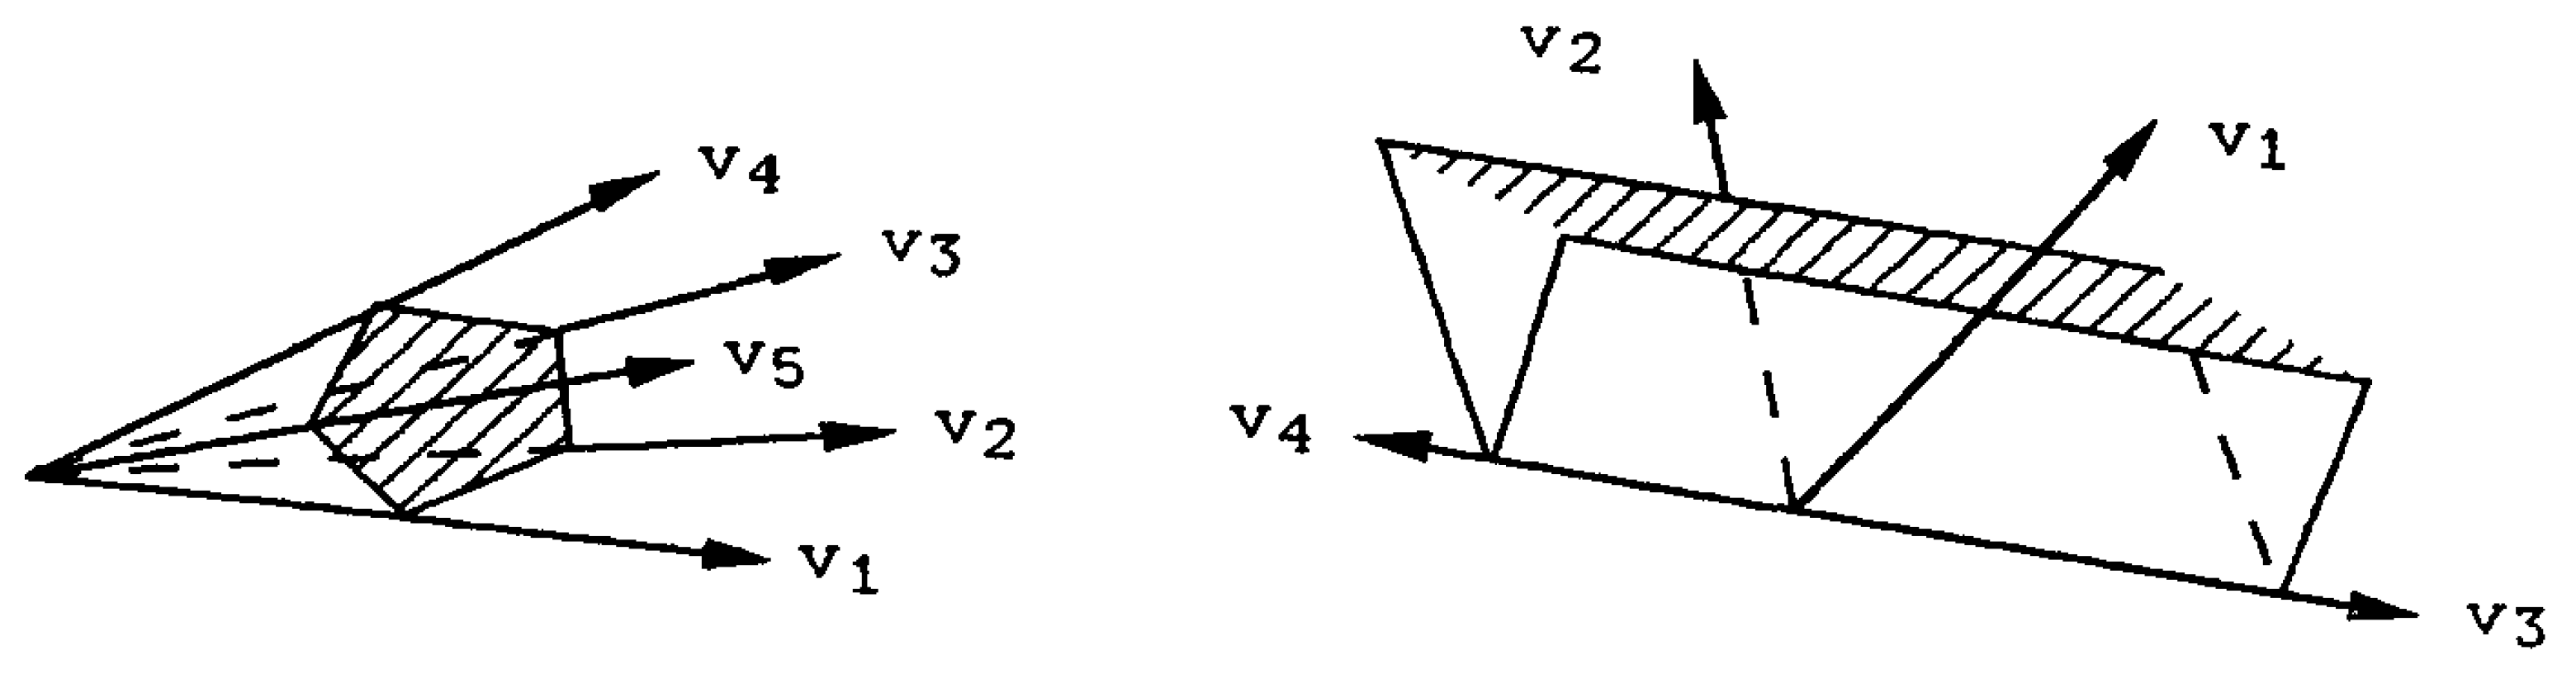
\includegraphics[width=0.8\textwidth]{../images/fultons_cones}
\caption{A strongly convex cone (left) and a non-strongly convex cone (right) \cite{Fulton93}.}
\label{figure:strongconvexity}
\end{figure}

Our goal is to give equivalent conditions for a cone to be strongly convex---the next lemma will help us do that.

For each face $\tau$ of $\sigma$, we define
$$\tau^\perp = \{u \in M_\RR : \langle u, v \rangle = 0 \text{ for all } v \in \tau\}.$$

\begin{lemma}\label{lemma:dualfaces}
If $\tau$ is a face of $\sigma$, then $\sigma^\vee \cap \tau^\perp$ is a face of $\sigma^\vee$, and
$$\dim(\tau) + \dim(\sigma^\vee \cap \tau^\perp) = \dim N_\RR.$$
Moreover, the map $\tau \mapsto \sigma^\vee \cap \tau^\perp$ is an inclusion-reversing bijection between the faces of $\sigma$ and the faces of $\sigma^\vee$.
In particular, the smallest face of $\sigma$ is $\sigma \cap (-\sigma) = (\sigma^\vee)^\vee \cap (\sigma^\vee)^\perp$.
\end{lemma}
\begin{proof}
See \cite[\S 1.2]{Fulton93} or \cite[\S 1]{Zaman13}.
\end{proof}

We can now give equivalent conditions for a cone to be strongly convex.

\begin{proposition}[{\cite[\S 1.2, Proposition 3]{Fulton93}}]\label{stronglyconvexprop}
For a convex polyhedral cone $\sigma$, the following conditions are equivalent:
\begin{enumerate}
\item $\sigma$ is strongly convex.
\item $\sigma \cap (-\sigma) = \{0\}$.
\item $\sigma$ contains no non-zero vector subspace of $N_\RR$.
\item $\sigma^\vee$ spans $M_\RR$.
\end{enumerate}
\end{proposition}
\begin{proof}
The largest vector subspace of $\sigma$ is $\sigma \cap (-\sigma)$, and this observation proves (2) and (3) are equivalent.
Lemma \ref{lemma:dualfaces} tells us $\sigma \cap(-\sigma)$ is also the smallest face of $\sigma$, so (1) and (2) are equivalent.
The dimension formula in Lemma \ref{lemma:dualfaces} applied to $\tau = \sigma \cap (-\sigma)$ says $\dim(\sigma \cap (-\sigma)) + \dim(\sigma^\vee) = \dim N_\RR$.
This gives the equivalence of (2) and (4).
\end{proof}





\subsection{Rational cones}\label{section:rationalcones}
To conclude this chapter, we introduce rational cones.
The cones used to study toric varieties are always rational (in addition to strongly convex).
Defining rational cones requires us to consider lattices in the vector spaces $N_\RR$ and $M_\RR$.

Recall $N_\RR$ and $M_\RR$ are dual vector spaces with dual pairing $\langle \cdot , \cdot \rangle : M_\RR \times N_\RR \to \RR$.
Now, let $N$ be a lattice in $N_\RR$.
This means $N$ is a free abelian subgroup of $N_\RR$ with rank $n = \dim N_\RR$ such that $\Span_\RR N = N_\RR$.
Concretely, $N$ is a lattice in $N_\RR$ if and only if there exists an $\RR$-basis for $N_\RR$ which is also a $\ZZ$-basis for $N$ \cite[\S 2.2]{Serre73}.
The relationship between $N$ and $N_\RR$ generalises the relationship between $\ZZ^n$ and $\RR^n$, and most of our examples will have $N = \ZZ^n$ and $N_\RR = \RR^n$ for simplicity.
We also let $M$ denote the dual lattice $\mathrm{Hom}_{\ZZ\text{-linear}}(N, \ZZ)$, which are the elements of $M_\RR = N_\RR^*$ taking integer values on $N$.

We say a polyhedral cone $\sigma$ is rational if its generators can be chosen from the lattice $N$.
All the examples of polyhedral cones we have seen are rational if our lattice is chosen to be $\ZZ^n$.
For example, when $N_\RR$ is $\RR^n$ and $N$ is $\ZZ^n$, the cone
$$\sigma = \Span_{\RR_{\ge 0}}\{e_1, \ldots, e_n\}$$
is rational, since the standard basis vectors $e_1, \ldots, e_n$ lie in $\ZZ^n$.
Similarly, when we choose $N_\RR$ to be $\RR^2$ and $N$ to be $\ZZ^2$, the cone
$$\sigma = \Span_{\RR_{\ge 0}}\{e_1, -e_1 + 2e_2\}$$
is rational.

%For an example of a cone which is not rational, take $N_\RR$ to be $\RR^2$ and $N$ to be $\ZZ^2$, and consider
%$$\sigma = \Span_{\RR_{\ge 0}}\{e_1, e_1 + \sqrt{2} e_2\}.$$
%Clearly the generator $e_1 + \sqrt{2} e_2$ does not lie in $N$.
%Further, it can be shown that no finite subset of $N$ generates $\sigma$, so it is not rational.

Here are two facts about rational cones which we will need when studying affine toric varieties:
\begin{enumerate}
\item If $\sigma$ is a rational cone, then its faces are too \cite[Proposition 2]{Fulton93}.
\item If $\sigma$ is a rational cone, then the dual $\sigma^\vee$ is rational (meaning generators of $\sigma^\vee$ can be chosen from the dual lattice $M$).
This fact can be proven using the algorithm we presented in \S \ref{section:dualdescription} to find generators of $\sigma^\vee$.
In particular, when the generators of $\sigma$ lie in $N$, the algorithm can be used to find generators for $\sigma^\vee$ in $M$. 
\end{enumerate}












\newpage
%\addtocontents{toc}{\vskip 1em}
\section{Affine toric varieties}\label{chapter:affinetoricvarieties}
Affine toric varieties are a class of algebraic varieties which are determined by a cone in a vector space.
There is a rich interplay between the algebraic geometry of the variety and the convex geometry of the cone.
Moreover, computations with the cone can often be done explicitly, which means toric varieties are useful to study as examples.

A toric variety $X$ is a normal variety containing an algebraic torus $T$ as a dense open subset, such that $T$ acts on $X$ by an action which extends the natural action of $T$ on itself.
This definition is straightforward to state, but makes no reference to a cone in a vector space, so the relationship with convex geometry is unclear.

In this chapter, we use the convex geometry from the previous chapter to define affine toric varieties using cones.
Afterwards, we prove some fundamental properties, such as the existence of a dense torus which acts on the variety, and computing singularities.

Throughout this chapter, $N$ is a lattice in the vector space $N_\RR$ and $M$ is the dual lattice in $M_\RR = N_\RR^*$ (c.f.\ \S \ref{section:rationalcones}).
A cone $\sigma$ is always assumed to be polyhedral, strongly convex and rational.

%To define an affine toric variety, we first associate a semigroup and semigroup algebra with a cone.
%An affine toric variety can then be defined as the spectrum of the semigroup algebra.
%The connections between a cone, its semigroup algebra, and the spectrum of the semigroup algebra give rise to the interplay between the geometries of the variety and the cone.





\subsection{Semigroups and semigroup algebras}
In this section, we associate two algebraic objects with a cone: a semigroup and its semigroup algebra.
We also explain when these objects are finitely generated.
We will use semigroup algebras to define affine toric varieties in \S \ref{section:affinetoricvarieties}.

Recall a semigroup is a set with an associative binary operation.
All the semigroups we consider are commutative, so we will write the operation additively.
If $S$ is a semigroup and $T$ is a finite subset of $S$, we say $T$ generates $S$ if every element in $S$ can be written as a sum of elements of $T$.
A map between semigroups with identity $\varphi : S \to T$ is a homomorphism if it preserves the identity and $\varphi(x + y) = \varphi(x) + \varphi(y)$ for all $x$ and $y$ in $S$.

%Now let $N$ be a lattice in $N_\RR$, with dual lattice $M$ in $M_\RR = N_\RR^*$.
Let $\sigma$ be cone in $N_\RR$.
The semigroup of $\sigma$ is defined as
$$S_\sigma := \sigma^\vee \cap M.$$
In other words, $S_\sigma$ is the set of lattice points in the dual cone of $\sigma$.
Since $S_\sigma$ is a subsemigroup of the lattice $M$, it is abelian.
Also, $S_\sigma$ contains $0$, meaning it is a semigroup with identity.\footnote{In the literature, it is conventional to call $S_\sigma$ a semigroup, even though it is in fact a monoid.}
The following result tells us when $S_\sigma$ is finitely generated:

\begin{theorem}[Gordan's lemma {\cite[\S 1.2]{Fulton93}}]\label{gordanslemma}
If $\sigma$ is a rational convex polyhedral cone, then $S_\sigma$ is a finitely generated semigroup.
\end{theorem}
\begin{proof}
We know $\sigma^\vee$ is polyhedral and rational because $\sigma$ is (c.f.\ Theorem \ref{theorem:farkas} and \S \ref{section:rationalcones}).
Then let $u_1, \ldots, u_s \in \sigma^\vee \cap M$ generate $\sigma^\vee$ as a cone.
Define
$$K = \left\{\sum_{i=1}^s t_i u_i : 0 \le t_i \le 1\right\} \subseteq M_\RR.$$
Since $K$ is compact and $M$ is discrete, the intersection $K \cap M$ is finite.
We claim $K \cap M$ generates $S_\sigma$.
%Note that $u_1, \ldots, u_s \in K \cap M$.
Suppose that $u \in S_\sigma$.
Then $u =\sum_{i=1}^s r_i u_i$ for some $r_i \in \RR_{\ge 0}$ since $u_1, \ldots, u_s$ generate $\sigma^\vee$.
Write each $r_i$ as $m_i + t_i$ for $m_i \in \ZZ_{\ge 0}$ and $0 \le t_i < 1$, so $u = \sum_{i=1}^s m_i u_i + \sum_{i=1}^s t_i u_i$.
Clearly $\sum_{i=1}^s t_i u_i$ lies in $K$.
Also, $\sum_{i=1}^s t_i u_i = u - \sum_{i=1}^s m_i u_i$ lies in $M$ since $u$ and $\sum_{i=1}^s m_i u_i$ lie in $M$ and $M$ is a group.
Then $\sum_{i=1}^s t_i u_i$ lies in $K \cap M$, and since $u_1, \ldots, u_s \in K \cap M$, we have $u = \sum_{i=1}^s m_i u_i + \sum_{i=1}^s t_i u_i \in \Span_{\ZZ_{\ge 0}} K \cap M$.
\end{proof}

Using the semigroup $S_\sigma = \sigma^\vee \cap M$, we can also construct the semigroup algebra $k[S_\sigma]$.
This construction is analogous to the construction of the group algebra using a group.
We now explain the details.

Given $S_\sigma$, the semigroup algebra $k[S_\sigma]$ is the algebra with basis of formal symbols
$$\{\chi^u : u \in S_\sigma\}.$$
The multiplication in $k[S_\sigma]$ is determined by addition in $S_\sigma$, in the following way:
$$\chi^u \chi^{u'} := \chi^{u + u'}.$$
The algebra $k[S_\sigma]$ is commutative and unital since $S_\sigma$ is.
Also, when $\sigma$ is rational, Gordan's lemma implies $S_\sigma$ and hence $k[S_\sigma]$ are finitely generated.
Specifically, if $u_1, \ldots, u_s$ generate $S_\sigma$, then $\chi^{u_1}, \ldots, \chi^{u_s}$ generate $k[S_\sigma]$.

As an example, let us consider the semigroup algebra corresponding to the trivial cone $\sigma = \{0\}$.
The dual cone $\sigma^\vee$ is all of $M_\RR$, so $S_\sigma = M_\RR \cap M = M$ and $k[S_\sigma]=k[M]$. 
Given a basis $\{e_1^*, \ldots, e_n^*\}$ for $M$, denote
$$X_i := \chi^{e_i^*} \in k[M].$$
As a semigroup, $M$ is generated by $\pm e_1^*, \ldots, \pm e_n^*$, so
$$k[M] = k[X_1, X_1^{-1}, \ldots, X_n, X_n^{-1}],$$
and $k[M]$ is the ring of Laurent polynomials in $X_1, \ldots, X_n$.
For any cone $\sigma$, the semigroup $S_\sigma$ is contained in $M$, so that $k[S_\sigma]$ is a subalgebra of $k[M]$. 
Then any semigroup algebra $k[S_\sigma]$ can be thought of as a subalgebra of the Laurent polynomials.
It follows that the semigroup algebra $k[S_\sigma]$ is always an integral domain.




\subsection{The definition of toric varieties}\label{section:affinetoricvarieties}
With the semigroup algebra defined, we are ready to define the affine toric variety corresponding to a cone.
After giving the definition, we provide some examples.

\begin{definition}
Let $\sigma$ be a rational cone in $N$.
The affine toric variety corresponding to $\sigma$ is
$$U_\sigma := \Spec(k[S_\sigma]).$$
\end{definition}

As $k[S_\sigma]$ is a finitely generated reduced $k$-algebra, $U_\sigma$ is an affine variety (c.f.\ \S \ref{section:themaximalspectrum}).
Furthermore, since $k[S_\sigma]$ is an integral domain, $U_\sigma$ is irreducible.
For example, if $\sigma = \{0\}$, then $S_{\{0\}}= M$, and
$$U_{\{0\}} = \Spec(k[X_1^\pm, \ldots, X_n^\pm]) = (k^\times)^n$$
is a torus.

To clarify the construction of the affine toric variety $U_\sigma$, we summarise the key steps, as some of the necessary definitions were introduced in the previous chapter.
\begin{enumerate}
\item Fix a pair of dual lattices $N$ and $M$ in the vector spaces $N_\RR$ and $M_\RR$.
Choose a rational cone in $N_\RR$, i.e., a polyhedral cone generated by elements of the lattice $N$.
\item Construct the semigroup $S_\sigma = \sigma^\vee \cap M$ and semigroup algebra $k[S_\sigma]$.
Since $\sigma$ is rational, Gordan's lemma ensures $k[S_\sigma]$ is finitely generated.
\item Set $U_\sigma := \Spec(k[S_\sigma])$.
\end{enumerate}
Given these steps, it is natural to ask why the semigroup is defined as the set of lattice points in the dual cone, rather than just the cone itself.
In \S \ref{section:facesandopenaffinesubsets}, we see why defining the semigroup in this way is a natural choice to make.

We now investigate the affine toric varieties arising from cones we saw in Example \ref{example:conesandduals} and Example \ref{example:3dconeanddual}.

\begin{example}\label{example:affinetoricvarieties}
\begin{enumerate}
\item
Suppose $1 \le r \le n$.
Consider $\sigma = \Span_{\RR_{\ge 0}}\{e_1, \ldots, e_r\}$ and its dual $\sigma^\vee = \Span_{\RR_{\ge 0}}\{e_1^*, \ldots, e_r^*, \pm e_{r+1}^*, \ldots, \pm e_n^*\}$.
The vectors $e_1^*, \ldots, e_r^*, \pm e_{r+1}^*, \ldots, \pm e_n^*$ generate $S_\sigma$ as a semigroup, so
$$k[S_\sigma] = k[\chi^{e_1^*}, \ldots, \chi^{e_r^*}, \chi^{\pm e_{r+1}^*}, \ldots, \chi^{\pm e_{n}^*}] = k[X_1, \ldots, X_r, X_{r+1}^\pm, \ldots, X_n^\pm],$$
and 
$$U_\sigma = \Spec(k[X_1, \ldots, X_r, X_{r+1}^\pm, \ldots, X_n^\pm])= k^r \times (k^\times)^{n-r}.$$

\item
Consider $\sigma = \Span_{\RR_{\ge 0}} \{e_1, - e_1 + 2 e_2\}$ and $\sigma^\vee = \Span_{\RR_{\ge 0}} \{2 e_1^* + e_2^*, e_2^*\}$, pictured below.
\begin{figure}[H]
    \centering
    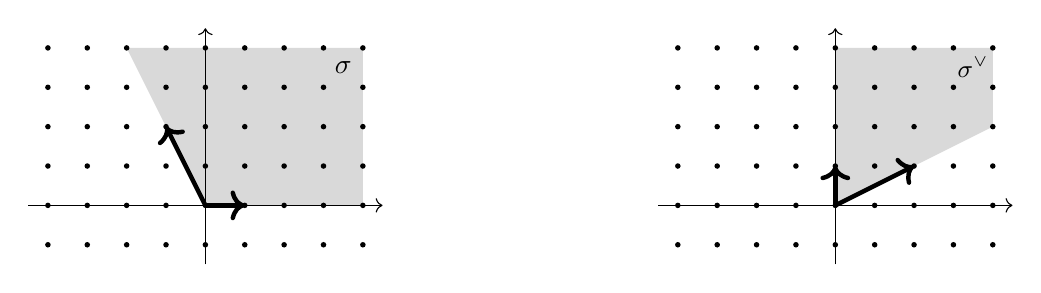
\begin{tikzpicture}
        % Left diagram
        \begin{scope}[shift={(-4,0)}]
            % Shaded area
            \fill[gray!30] (0,0) -- (-1,2) -- (2,2) -- (2,0) -- cycle;
            
            % Axes
            \draw[->] (-2.25,0) -- (2.25,0);
            \draw[->] (0,-0.75) -- (0,2.25);
            
            % Lattice points
            \foreach \x in {-2,-1.5,-1,-0.5,0,0.5,1,1.5,2}
                \foreach \y in {-0.5,0,0.5,1,1.5,2}
                    \fill (\x,\y) circle (1pt);

            % Vectors
            \draw[->, ultra thick] (0,0) -- (0.5,0);
            \draw[->, ultra thick] (0,0) -- (-0.5,1);
            \node at (1.75, 1.75) {$\sigma$};
        \end{scope}
        
        % Right diagram
        \begin{scope}[shift={(4,0)}]
            % Shaded area
            \fill[gray!30] (0,0) -- (0,2) -- (2,2) -- (2, 1) -- cycle;
            
            % Axes
            \draw[->] (-2.25,0) -- (2.25,0);
            \draw[->] (0,-0.75) -- (0,2.25);
            
            % Lattice points
            \foreach \x in {-2,-1.5,-1,-0.5,0,0.5,1,1.5,2}
                \foreach \y in {-0.5,0,0.5,1,1.5,2}
                    \fill (\x,\y) circle (1pt);

            % Vectors
            \draw[->, ultra thick] (0,0) -- (0,0.5);
            \draw[->, ultra thick] (0,0) -- (1,0.5);
            \node at (1.75, 1.75) {\small{$\sigma^\vee$}};
        \end{scope}
    \end{tikzpicture}
\end{figure}
\noindent
While $\{2 e_1^* + e_2^*, e_2^*\}$ generates $\sigma^\vee$ as a cone, it does not generate $S_\sigma$ as a semigroup, since not every element in $S_\sigma$ lies in $\Span_{\ZZ_{\ge 0}} \{2 e_1^* + e_2^*,  e_2^*\}$.
For example, $e_1^* + e_2^* \in S_\sigma$, but $e_1^* + e_2^* \notin \Span_{\ZZ_{\ge 0}} \{2 e_1^* + e_2^*,  e_2^*\}.$
However, $\{e_2^*, 2 e_1^* + e_2^*,  e_1^* + e_2^*\}$ generates $S_\sigma$.
Then,
\begin{align*}
	\qquad k[S_\sigma] = k[\chi^{e_2^*}, \chi^{2 e_1^* + e_2^*}, \chi^{e_1^* + e_2^*}] &= k[X_2, X_1^2 X_2, X_1 X_2] \cong k[X, Y, Z] / (X Y - Z^2),
\end{align*}
and
$$U_\sigma = \Spec(k[X, Y, Z] / (XY - Z^2) )= \bV(X Y - Z^2).$$

\item
Consider $\sigma = \Span_{\RR_{\ge 0}}\{ e_1, e_2, e_1+e_3, e_2 + e_3\}$ and $\sigma^\vee = \Span_{\RR_{\ge 0}} \{e_1^*, e_2^*, e_3^*, e_1^* +e_2^* - e_3^*\}.$
We have 
\begin{align*}
	k[S_\sigma] &= k[\chi^{e_1^*}, \chi^{e_2^*}, \chi^{e_3^*}, \chi^{e_1^* +e_2^* - e_3^*}] \\
	&= k[X_1, X_2, X_3, X_1 X_2 X_3^{-1}] \\
	&\cong k[X, Y, Z, W]/(XY - ZW),
\end{align*}
and so
$$U_\sigma = \Spec(k[X, Y, Z, W] / (XY - ZW) ) = \bV(XY-ZW).$$
\end{enumerate}
\end{example}





\subsection{Points of toric varieties}\label{section:points}
We have seen how points in affine varieties correspond to maximal ideals in the coordinate ring (c.f.\ \S \ref{section:thenullstellensatz} and \S \ref{section:themaximalspectrum}).
Our goal in this section is to explain the different ways of viewing points in affine toric varieties.
The fact that the coordinate ring of an affine toric variety arises as a semigroup algebra affords us another perspective of points, namely as semigroup homomorphisms.
Later, in \S\ref{section:thetorusaction}, we will use the semigroup homomorphism point of view to define a torus action on an affine toric variety.

\begin{proposition}[{\cite[Proposition 1.3.1]{CLS11}}]\label{proposition:pointbijections}
Let $\sigma$ be a cone in $N$ and $U_\sigma = \Spec(k[S_\sigma])$ the associated affine toric variety.
The following sets are in bijection:
\begin{enumerate}
\item The set of points of $U_\sigma$.
\item The set of maximal ideals of $k[S_\sigma]$.
\item The set of $k$-algebra homomorphisms $k[S_\sigma] \to k$.
\item The set of semigroup homomorphisms $S_\sigma \to k$.\footnote{Here, $k$ is considered as a semigroup under multiplication.}
\end{enumerate}
\end{proposition}

\begin{proof}
The bijection between (1) and (2) from the definition of the maximal spectrum.
The bijection between (1) and (3) is explained in \cite[3.28]{Milne13}.

We explain the bijection between (3) and (4) now.
Given a $k$-algebra homomorphism $\varphi : k[S_\sigma] \to k$, define a semigroup homomorphism $x : S_\sigma \to k$ by $x(u) := \varphi(\chi^u)$.
Conversely, a semigroup homomorphism $x : S_\sigma \to k$ determines a $k$-algebra homomorphism $\varphi : k[S_\sigma] \to k$, defined on basis elements by $\varphi(\chi^u) := x(u)$.
These maps are mutually inverse and are hence bijections.
\end{proof}

Let us take a closer look at the above bijections when $U_\sigma = U_{\{0\}} = (k^\times)^n$.

\begin{example}
We saw in \S \ref{section:affinetoricvarieties} that when $\sigma = \{0\}$, the semigroup $S_\sigma$ is generated by $\pm e_1^*, \ldots, \pm e_n^*$, where $\{e_1^*, \ldots, e_n^*\}$ is a basis of $M$.
We write $X_i := \chi^{e_i^*}$ so that $k[S_\sigma] = k[X_1^{\pm}, \ldots, X_n^\pm]$.
We now detail the sets named in Proposition \ref{proposition:pointbijections}.
\begin{enumerate}
\item The set of points of $U_\sigma = (k^\times)^n$ is $\{(a_1, \ldots, a_n) : a_i \ne 0\}$ (when considering $(k^\times)^n$ embedded in $\AA^n$).
\item For brevity, let $A$ denote the polynomial ring $k[X_1, \ldots, X_n]$ and $h$ the element $X_1 \cdots X_n$.
We know $k[S_\sigma]$ is the localisation $A_h$ (c.f.\ \S\ref{section:opensubsetsofalgebraicsets}).
Maximal ideals in $A_h$ are all of the form $\frakm A_h$, where $\frakm$ is a maximal ideal of $A$ not containing $h$ (c.f.\ Proposition \ref{proposition:localizationideals}).
The Nullstellensatz tells us every maximal ideal of $A$ is of the form $\frakm_a = (X_1 - a_1, \ldots, X_n - a_n)$ for some $a = (a_1, \ldots, a_n) \in \AA^n$.
One readily checks $\frakm_a$ does not contain $h$ if and only if each $a_i$ is non-zero.
Then the set of maximal ideals in $k[S_\sigma]$ is $$\{\frakm_a A_h : a = (a_1, \ldots, a_n) \in (k^\times)^n\}.$$
\item The $k$-algebra homomorphism $k[S_\sigma] \to k$ corresponding to the maximal ideal $\frakm_a$ is the unique map with kernel $\frakm_a$.
This map is defined on generators by $X_i^\pm \mapsto a_i^\pm$.
\item The semigroup homomorphism corresponding to the $k$-algebra homomorphism in (3) is
$$S_\sigma = M \to k, \qquad \pm e_i^* \mapsto a_i^\pm.$$
Note since $M$ is a group, every element in the image of a semigroup homomorphism $M \to k$ is invertible, and such a map is in fact a homomorphism of groups $M \to k^\times$.
\end{enumerate}
\end{example}

Let us consider how multiplication of points in $(k^\times)^n$ looks from the perspective of homomorphisms---this will be useful when defining the torus action in \S \ref{section:thetorusaction}.
Suppose $x : M \to k^\times$ and $y : M \to k^\times$ are homomorphisms given by $x(e_i^*) = a_i$ and $y(e_i^*) = b_i$.
Then $x$ and $y$ correspond to the points $(a_1, \ldots, a_n)$ and $(b_1, \ldots, b_n)$, respectively.
The product $(a_1 b_1, \ldots, a_n b_n)$ corresponds to the product of homomorphisms
$$xy : M \to k^\times, \qquad (xy)(e_i^*) := a_i b_i.$$




\subsection{Faces and open affine subsets}\label{section:facesandopenaffinesubsets}
In this section, we show how faces of a cone correspond to open affine subsets in an affine toric variety.
In particular, we will see that every affine toric variety contains a torus as a dense open subset.

If $\tau$ is a face of $\sigma$, then $\tau^\vee \supseteq \sigma^\vee$ and $S_\tau \supseteq S_\sigma$, since dualising reverses inclusion.
The inclusion of semigroups $S_\sigma \hookrightarrow S_\tau$ induces the inclusion of $k$-algebras $k[S_\sigma] \hookrightarrow k[S_\tau]$, and hence a morphism $U_\tau \to U_\sigma$ (c.f.\ \S \ref{section:morphisms}).
The main result of this section is to show this morphism embeds $U_\tau$ as a principal open subset of $U_\sigma$.

\begin{proposition}\label{proposition:facesopensubsets}
If $\tau$ is a face of $\sigma$, then the map $U_\tau \to U_\sigma$ embeds $U_\tau$ as a principal open subset of $U_\sigma$.
\end{proposition}

The above proposition is one reason why we use dual cones to define toric varieties: smaller faces in a cone correspond to smaller open subsets in the variety.
In other words, using the dual gives an inclusion-preserving correspondence between faces and open subsets.

Before proving Proposition \ref{proposition:facesopensubsets}, we consider some of its consequences:
\begin{enumerate}
\item The torus $U_{\{0\}} = (k^\times)^n$ is a dense open subset of $U_\sigma$. The cone $\sigma$ is strongly convex so $\{0\}$ is a face. Then the proposition says $U_{\{0\}}$ is a principal open subset of $U_\sigma$, and open subsets of an irreducible affine variety are dense (c.f.\ \ref{}).
\item The dimension of $U_\sigma$ is $\dim N_\RR = n$. We have $\dim U_\sigma = \dim (k^\times)^n = n$ because the dimension of a principal open subset equals the dimension of the variety (c.f.\ \ref{}).
\end{enumerate}
\noindent These important consequences rely on $\sigma$ being strongly convex, justifying why we make this assumption about our cones.

%Recall that $\sigma$ is strongly convex so $\{0\}$ is a face.
%The proposition then says that $U_\sigma$ has the torus $U_{\{0\}} = (k^\times)^n$ as a principal open subset.
%In particular, since $U_\sigma$ is irreducible, $(k^\times)^n$ is dense in $U_\sigma$ (c.f.\ \ref{}).
%As a consequence, we see $\dim U_\sigma= \dim (k^\times)^n = n$, since the dimension of a principal open subset equals the dimension of the variety (c.f.\ \ref{}).
%The strongly convex assumption on our cones is then useful for two reasons: it ensures the variety has a torus as a dense open subset, and it means the dimension of the variety agrees with the dimension of the lattice.

For the rest of this thesis, we use $T_N$ to denote the torus $U_{\{0\}}$, which is embedded in every affine toric variety associated with a cone in $N$.
In \S \ref{section:thetorusaction}, we will see explicit embeddings of $T_N$ in $U_\sigma$, after developing the theory of how $T_N$ acts on $U_\sigma$.

To prove Proposition \ref{proposition:facesopensubsets}, we start with a lemma that describes the relationship between the semigroups $S_\tau$ and $S_\sigma$, which elucidates the relationship between $k[S_\tau]$ and $k[S_\sigma]$.

\begin{lemma}
If $\tau$ is a face of $\sigma$, then $\tau = \sigma \cap u^\perp$ for some $u \in S_\sigma$.
Moreover, we have $S_\tau =S_\sigma + \ZZ_{\ge 0} \cdot (-u).$
\end{lemma}
\begin{proof}
By definition, $\tau = \sigma \cap u^\perp$ for some $u \in \sigma^\vee$, but we need to construct such a $u$ in the lattice to conclude $u \in S_\sigma$.
Notice $\sigma^\vee \cap \tau^\perp$ is a face in the rational cone $\sigma^\vee$, so there are $u_1, \ldots, u_s$ lying in the lattice which generate $\sigma^\vee \cap \tau^\perp$.
We define $u := \sum_{i=1}^s u_i \in S_\sigma$.
To see $\tau \subseteq \sigma \cap u^\perp$, observe that if $v$ lies in $\tau$, then $\langle u, v\rangle = 0$, since $u$ lies in $\sigma^\vee \cap \tau^\perp$.
Conversely, suppose $v$ lies in $\sigma \cap u^\perp$.
It follows $\langle u_i, v \rangle = 0$ for each $i$, and hence $v \in (\sigma^\vee \cap \tau^\perp)^\perp$.
Then $v$ lies in $\sigma \cap (\sigma^\vee \cap \tau^\perp)^\perp$, and Lemma \ref{lemma:dualfaces} implies  $\tau = \sigma \cap (\sigma^\vee \cap \tau^\perp)^\perp$.

To see $S_\tau \subseteq S_\sigma + \ZZ_{\ge 0} \cdot (-u)$, let $w \in S_\tau$, and suppose $v_1, \ldots, v_r$ lie in the lattice and generate $\sigma$ as a cone.
For any $v = \sum_{i=1}^r t_i v_i$ in $\sigma$ (where each $t_i \ge 0$) and any positive integer $p$, we have
$$\langle w + pu, v\rangle = \sum_{i=1}^r t_i \left( \langle w, v_i \rangle + p \langle u, v_i \rangle \right).$$
We want to choose $p$ so that each summand is non-negative to ensure $\langle w+pu, v \rangle \ge 0$.
For all $i$, there holds $\langle u, v_i \rangle \ge 0$.
Thus, when $\langle w, v_i \rangle \ge 0$, the $i^\text{th}$ summand is non-negative.
If $\langle w, v_i\rangle < 0$, then $v_i$ does not lie in $\tau$.
In this case, we must have $\langle u, v_i\rangle \ge 1$, because $v_i \notin \tau$ means $\langle u, v_i \rangle \ne 0$, and $\langle u, v_i \rangle$ lies in $\ZZ$ since $u$ and $v_i$ are both lattice points.
It follows that if $p := \max_i |\langle u, v_i\rangle|$, then each summand is non-negative.
Thus, $w + pu \in S_\sigma$ and $w \in S_\sigma + \ZZ_{\ge 0} \cdot (-u).$

Conversely, if $w - pu \in S_\sigma + \ZZ_{\ge 0} \cdot (-u)$, then for any $v \in \tau$, we have $\langle w - pu, v\rangle = \langle w, v \rangle \ge 0$, and so $w - pu \in S_\tau$.
\end{proof}

We are now ready to prove Proposition \ref{proposition:facesopensubsets}.

\begin{proof}[{Proof of Proposition \ref{proposition:facesopensubsets}}]
The lemma yields $u$ in $S_\sigma$ such that $\tau = \sigma \cap u^\perp$ and $S_\tau = S_\sigma + \ZZ_{\ge 0} \cdot (-u)$.
Then any basis element of $k[S_\tau]$ can be written $\chi^{w - pu} = \frac{\chi^w}{\chi^{pu}}$ for some $w \in S_\sigma$ and $p \in \ZZ_{\ge 0}$.
It follows that $k[S_\tau]$ is the localisation $k[S_\sigma]_{\chi^u}$, and the inclusion $k[S_\sigma] \hookrightarrow k[S_\tau] = k[S_\sigma]_{\chi^u}$ is the localisation homomorphism.
Proposition \ref{proposition:localisationembedding} tells us that the corresponding morphism $U_\tau \to U_\sigma$ embeds $U_\tau$ as a principal open subset of $U_\sigma$.
\end{proof}

\subsection{The torus action}\label{section:thetorusaction}
In this section, we define an action of the dense torus on an affine toric variety.
This means the affine toric varieties we have defined in terms of cones are toric varieties in the sense mentioned in the introduction to this chapter.
The torus action is defined using the semigroup homomorphism perspective of points.
Afterwards, we check this defines a group action which extends the natural action of a torus on itself.
We conclude the section with examples.

Let $\sigma$ be a cone in $N$.
We refer to semigroup homomorphisms as points, using the identification established in \S\ref{section:points}.
Let $t : M \to k^\times$ and $x : S_\sigma \to k$ be points in $T_N$ and $U_\sigma$, respectively.
The action map $\varphi : T_N \times U_\sigma \to U_\sigma$ is defined by 
$$(t, x) \mapsto (u \mapsto t(u)x(u)).$$
We write $t \cdot x$ for the image of $(t, x)$.
Then $t \cdot x$ is simply the product of semigroup homomorphisms.
We now prove $\varphi$ is a group action extending the natural action of $T_N$ on itself.

\begin{proposition}
The map $\varphi : T_N \times U_\sigma \to U_\sigma$ is a group action.
Moreover, under the identification of $T_N$ with an open subset of $U_\sigma$, $\varphi$ extends the natural action of $T_N$ on itself by left multiplication.
\end{proposition}
\begin{proof}
To prove $\varphi$ is an action of the algebraic group $T_N$, we must show $\varphi$ is a morphism of varieties and also a group action.

To see $\varphi$ is a morphism, we check its pullback is a $k$-algebra homomorphism.
Recall that to evaluate the regular function $\chi^u \in k[S_\sigma]$ at $x : S_\sigma \to k$, we compute $\chi^u(x) = x(u)$.
We see
$$\varphi^*(\chi^u)(t, x) = \chi^u(t\cdot x) = (tx)(u) = (\chi^u \otimes \chi^u)(t,x).$$
Then $\varphi^* : k[S_\sigma] \to k[M] \otimes k[S_\sigma]$ is given by $\chi^u \mapsto \chi^u \otimes \chi^u$, which is clearly a homomorphism.

The semigroup homomorphism corresponding to the identity in $T_N$ is the trivial homomorphism $1_{T_N} : M \to k^\times$.
Using this, and the fact that the product in $T_N$ is given by the product of semigroup homomorphisms (c.f.\ \S \ref{section:points}), it is straightforward to check $1 \cdot x = x$ and $t_1\cdot(t_2\cdot x) = (t_1t_2)\cdot x$.
Then $\varphi$ is a group action.

We also need to check this action extends the natural action of $T_N$ on itself by left multiplication.
From \S\ref{section:facesandopenaffinesubsets}, we have a map $\iota : T_N \hookrightarrow U_\sigma$ embedding $T_N$ as an open subset of $U_\sigma$.
We need to check $t_1 \cdot \iota(t_2) = \iota(t_1 t_2)$ for any two points $t_1$ and $t_2$ in $T_N$.
Since the action is defined using semigroup homomorphisms, we need to understand $\iota$ at the level of semigroup homomorphisms.
If $t : M \to k^\times$ is a point in $T_N$, then $\left. t \right|_{S_\sigma} : S_\sigma \to k$ is a point in $U_\sigma$.
This is a natural guess for how $\iota$ is evaluated on semigroup homomorphisms.
Evaluating this restriction map at $t : M \to k^\times$, then applying a regular function $\chi^u \in k[S_\sigma]$, gives
% This restriction of semigroup homomorphism map composed with a regular function $\chi^u \in k[S_\sigma]$, evaluated at $t : M \to k^\times$, is
$$\chi^u(\left. t \right|_{S_\sigma}) = \left. t \right|_{S_\sigma}(u) = t(u) = \chi^u(t).$$
This agrees with $\iota^*(\chi^u)(t)$, so our guess is correct.
Then $t_1 \cdot \iota(t_2)$ and $\iota(t_1 t_2)$ both equal $\left. t_1 t_2 \right|_{S_\sigma}$.
\end{proof}

We now examine this torus action for the toric varieties we saw in Example \ref{example:affinetoricvarieties}.

\begin{example}
\begin{enumerate}
\item Consider $\sigma = \Span_{\RR_{\ge 0}}\{e_1, \ldots, e_n\}$ and $S_\sigma = \Span_{\ZZ_{\ge 0}}\{e_1^*, \ldots, e_n^*\}$.
Then a semigroup homomorphism $x : S_\sigma \to k$ is given by $e_i^* \mapsto a_i$ for some $(a_1, \ldots, a_n) \in \AA^n$.
Points in the torus $t : M \to k^\times$ are given by $e_i^* \mapsto b_i$ for some $(b_1, \ldots, b_n)\in(k^\times)^n$.
We then see the embedding of $T_N$ into $\AA^n$ is the usual one.
The torus action is given by $t\cdot x : S_\sigma \to k$, where $e_i^* \mapsto a_i b_i$, so $T_N$ acts on $\AA^n$ by component-wise multiplication.
\item Consider $\sigma = \Span_{\RR_{\ge 0}} \{e_1, -e_1 + 2 e_2\}$ and $S_\sigma = \Span_{\ZZ_{\ge 0}}\{e_2^*, 2e_1^*+e_2^*, e_1^*+e_2^*\}$.
Any point in $U_\sigma = \bV(XY- Z^2)$ is a map $p : S_\sigma \to k$, given on the generators by
$$e_2^* \mapsto x, \qquad 2e_1^*+e_2^* \mapsto y, \qquad e_1^*+e_2^* \mapsto z,$$
subject to the restraint $xy=z^2$ so that the map is a homomorphism.
A point in the torus $T_N = (k^\times)^2$ is a map $t : M \to k^\times$ given by
$$e_1^* \mapsto a, \qquad e_2^* \mapsto b.$$
The restriction $\left. t \right|_{S_\sigma}$ gives the embedding $T_N \hookrightarrow U_\sigma$.
This is the homomorphism $\left. t \right|_{S_\sigma} : S_\sigma \to k$ given by
$$e_2^* \mapsto b, \qquad 2e_1^*+e_2^* \mapsto a^2 b, \qquad e_1^*+e_2^* \mapsto ab.$$
We see the embedding $T_N \hookrightarrow U_\sigma$ is given by $(a, b) \mapsto (b, a^2 b, ab)$.
This means $T_N$ is all the points in $U_\sigma$ with non-zero coordinates.
Furthermore, $t\cdot p = tp : S_\sigma \to k$ is given by
$$e_2^* \mapsto bx, \qquad 2e_1^*+e_2^* \mapsto a^2 by, \qquad e_1^*+e_2^* \mapsto abz.$$
In other words, the action can be written explicitly as
$$(b, a^2b, ab) \cdot (x, y, z) = (bx, a^2by, abz).$$
\end{enumerate}
\end{example}


\subsection{Singularities}
In this section, we characterise when affine toric varieties are non-singular using their cones.

\begin{theorem}\label{theorem:singularities}
An affine toric variety $U_\sigma$ is non-singular if and only if $\sigma$ is generated by a subset of a basis for the lattice $N$.
In this case,
$$U_\sigma \cong k^r \times (k^\times)^{n-r},$$
where $r = \dim(\sigma)$.
\end{theorem}

We have already seen that $U_\sigma$ is isomorphic to $k^r \times (k^\times)^{n-r}$ when $\sigma$ is generated by $r$ basis vectors of $N$ (c.f.\ Example \ref{example:affinetoricvarieties}).
Therefore, it remains to prove the converse.
To do so, we need to consider the so-called distinguished point $x_\sigma$ in $U_\sigma$.
This point is given by the map of semigroups
$$x_\sigma : S_\sigma \to k, \qquad x_\sigma(u) := \begin{cases} 1 & \text{if } u \in \sigma^\perp, \\ 0 & \text{otherwise.} \end{cases}$$
This is a homomorphism since $\sigma^\perp$ is a face of $\sigma^\vee$, so a sum of two elements in $S_\sigma$ lies in $\sigma^\perp$ if and only if each element lies in $\sigma^\perp$ \cite[\S 2.1]{Fulton93}.
The strategy of the proof of Theorem \ref{theorem:singularities} is to show that if $U_\sigma$ is non-singular at $x_\sigma$, then $\sigma$ is generated by a subset of a basis for $N$.

\begin{proof}
We consider the case when $\sigma$ is non-degenerate. For a proof of the degenerate case, see \cite[\S 2.1]{Fulton93}.

As $\sigma$ spans $N_\RR$, we have $\sigma^\perp = \{0\}$.
Thus, $x_\sigma(u)$ equals 1 if $u=0$ and equals 0 if $u \ne 0$.
The maximal ideal $\frakm$ corresponding to $x_\sigma$ is the ideal of regular functions vanishing at $x_\sigma$.
As $\chi^u(x_\sigma) = x_\sigma(u)$, we see $\frakm$ is generated by the $\chi^u$ for all $u \in S_\sigma \setminus \{0\}$.
Hence, $\frakm^2$ is generated by the $\chi^u$ such that $u$ is a sum of two elements in $S_\sigma \setminus \{0\}$.
We see $\frakm / \frakm^2$ has the basis 
$$\{\chi^u + \frakm^2 : u \in (S_\sigma)_{\text{irred}}\},$$
where $(S_\sigma)_{\text{irred}}$ is the set
$$(S_\sigma)_{\text{irred}} = \{u \in S_\sigma \setminus \{0\} : u \text{ is not a sum of two elements in } S_\sigma\setminus\{0\}\}.$$
Since $U_\sigma$ is non-singular, the Zariski tangent space $(\frakm/\frakm^2)^*$ has dimension $n = \dim(U_\sigma)$, and thus $|(S_\sigma)_{\text{irred}}| = n$.

We now consider which elements lie in $(S_\sigma)_{\text{irred}}$.
Any edge (i.e., a one-dimensional face) of $\sigma^\vee$ can be generated by a single lattice element.
If $p u$ lies in $S_\sigma$ for some $p \in \ZZ_{> 0}$ and $u \in M$, then $u$ lies in $S_\sigma$, since $S_\sigma$ is the intersection of $M$ with a cone.
Then for any edge, there exists a unique $u \in S_\sigma$ generating the edge which is not the sum of two non-zero elements in the edge.
Such a $u$ is called a minimal edge generator.
%It follows that an edge of $\sigma$ is generated by a unique $u$ lying in $S_\sigma$ which is not the sum of two non-zero elements lying in the edge---we call such a $u$ an edge generator.
The minimal edge generators lie in $(S_\sigma)_{\text{irred}}$ \cite[Proposition 1.2.23]{CLS11} and generate the cone \cite[Lemma 1.2.15]{CLS11}.
Since $\sigma$ is strongly convex, $\sigma^\vee$ spans $M_\RR$ and there must be $n$ minimal edge generators.
We conclude $(S_\sigma)_{\text{irred}}$ is the set of minimal edge generators.

Then $(S_\sigma)_{\text{irred}}$ is a set of $n$ linearly independent lattice points that generate the cone.
To complete the proof, we just need to show $(S_\sigma)_{\text{irred}}$ generates $M$ as a group.
This follows from two facts: $(S_\sigma)_{\text{irred}}$ generates $S_\sigma$ \cite[Proposition 1.2.23]{CLS11}, and $S_\sigma + (-S_\sigma) = M$.
The latter is true because $\sigma^\vee$ spans $M_\RR$.
\end{proof}

We revisit the singular affine toric varieties we saw in Example \ref{example:affinetoricvarieties} to see how the cone generators detect when the variety is singular.

\begin{example}
\begin{enumerate}
\item If $\sigma = \Span_{\RR_{\ge 0}}\{e_1, e_2, e_1+e_3, e_2+e_3\}$, then
$$U_\sigma = \bV(XY - ZW).$$
Note $U_\sigma$ is singular since all partial derivatives of $XY-ZW$ vanish at the origin.
The generating set $\{e_1, e_2, e_1+e_3, e_2+e_3\}$ is not a basis for $\ZZ^3$ as it contains four vectors.
\item If $\sigma = \Span_{\RR_{\ge 0}}\{e_1, -e_1+2e_2\}$, then
$$U_\sigma = \bV(XY - Z^2).$$
Again, $U_\sigma$ is singular since all partial derivatives of $XY-Z^2$ vanish at the origin.
Notice that any point in the $\ZZ$-span of the generating set $\{e_1, -e_1+2e_2\}$ has even $y$-component; thus, the generating set is not a basis for $\ZZ^2$.
\end{enumerate}
\end{example}








\newpage
%\addtocontents{toc}{\vskip 1em}
\section{GIT quotients as toric varieties}\label{chapter:gitquotientsastoricvarieties}
%In this chapter, we introduce the affine GIT quotient and give examples.
%One example we give is $\frakg \git T$ for $G = \GL_2(\CC)$.
%We then compute a basis of $\CC[\frakg]^T$ for general $G$.
%Finally, we find generators for the invariant ring $\CC[\frakg]^T$ when $G = \GL_3(\CC)$.
%Throughout this chapter, many technical details may be missing;
%our focus is on understanding specific examples which can guide our investigation of $\frakg \git T$ for general $G$.
%




\subsection{Algebraic groups and their actions}
%\subsection{Reductive groups}





\subsection{The affine GIT quotient}
Let $G$ be an affine algebraic group over $\CC$ and $X = \Spec(A)$ a complex affine variety with coordinate ring $A$.
Suppose that $G$ acts on $X$.
Recall that the $G$-invariant functions on $X$ are
$$A^G := \{f \in A : f(g \cdot P) = f(P) \text{ for all } g \in G \text{ and } P \in X\}.$$

\begin{definition}
The GIT quotient is defined as
$$X \git G := \Spec(A^G).$$
\end{definition}

Note that points in $X \git G$ are not necessarily in bijection with the orbits $X / G$, but the GIT quotient defines a quotient variety even when $X / G$ does not have the structure of an affine variety.
Let us see some examples of GIT quotients:

\begin{example}\label{gitexamples}
\begin{enumerate}
\item
Consider the group $\CC^\times$ acting on the affine space $\CC^2$ by 
$$
\hspace{\labelwidth} \hspace{\labelsep} \hspace{\leftmargin}
t \cdot (x, y) = (tx, t^{-1}y), \qquad t \in \CC^\times, (x, y) \in \CC^2.
$$
Suppose a polynomial $p$ has coefficients $a_{ij} \in \CC$ such that
$$
\hspace{\labelwidth} \hspace{\labelsep} \hspace{\leftmargin}
p(X, Y) = \sum_{i, j} a_{ij} X^i Y^j.
$$
Then $p$ is $\CC^\times$ invariant if and only if for all $t \in \CC^\times$,
$$
\hspace{\labelwidth} \hspace{\labelsep} \hspace{\leftmargin}
\sum_{i,j} a_{ij} X^i Y^j = \sum_{i,j} a_{ij} t^{i-j} X^i Y^j.
$$
This is equivalent to having $a_{ij} \ne 0$ if and only if $i = j$.
Thus, we have that
$$
\hspace{\labelwidth} \hspace{\labelsep} \hspace{\leftmargin}
\CC[X, Y]^{\CC^\times} = \CC[XY], \qquad \text{and} \qquad \CC^2 \git \CC^\times = \Spec(\CC[XY]) \cong \CC.
$$

\item
Let $G$ be $\GL_2(\CC)$ and $T$ the maximal torus of invertible diagonal matrices in $G$.
The action of $G$ on its Lie algbera $\frakg = \frakg \frakl_2(\CC)$ by conjugation induces an action of $T$ on $\frakg$.
Specifically, if $\begin{pmatrix} a & 0 \\ 0 & b \end{pmatrix} \in T$ and $\begin{pmatrix} x & y \\ z & w \end{pmatrix} \in \frakg$, 
$$\begin{pmatrix} a & 0 \\ 0 & b \end{pmatrix} \cdot \begin{pmatrix} x & y \\ z & w \end{pmatrix} 
= \begin{pmatrix} a & 0 \\ 0 & b \end{pmatrix} \begin{pmatrix} x & y \\ z & w \end{pmatrix} \begin{pmatrix} a & 0 \\ 0 & b \end{pmatrix}^{-1}
= \begin{pmatrix} x & a b^{-1} y \\ a^{-1} b z & w \end{pmatrix}.$$
Let $X \in \CC[\frakg]$ be the coordinate function defined by $X \left(\begin{pmatrix} x & y \\ z & w \end{pmatrix}  \right) := x$, and define $Y, W, Z \in \CC[\frakg]$ analogously.
Then $\CC[\frakg] = \CC[X, Y, Z, W]$.
Since $T$ acts trivially on the diagonal entries of an element in $\frakg$, $X, W \in \CC[\frakg]^T$.
The action on the off-diagonal entries is analogous to the action in part (1);
by the same argument that we used in part (1), a polynomial $p$ is invariant if and only if for each monomial in $p$, the exponent of $Y$ is equal to the exponent of $Z$.
Therefore,
$$\CC[\frakg]^T = \CC[X, W, YZ], \qquad \text{and} \qquad \frakg \git T = \Spec(\CC[X, W, YZ]) \cong \CC^3.$$

\item
Let $S_2 = \langle \sigma \, | \, \sigma^2 = 1 \rangle$ act on $\CC^2$ by
$$
\hspace{\labelwidth} \hspace{\labelsep} \hspace{\leftmargin}
\sigma \cdot (x, y) = (y, x).
$$
Polynomials which are invariant under the induced action on $\CC[X, Y]$ are called symmetric polynomials.
We compute $\CC[X, Y]^{S_2}$, i.e., the ring of symmetric polynomials in two variables;
this computation is a special case of the fundamental theorem of symmetric polynomials, which characterises $\CC[X_1, \ldots, X_n]^{S_n}$ when $S_n$ acts on $\CC^n$ by permuting coordinates (see \cite[Chapter IV, \S 6]{Lang02} for a proof of the general theorem).

We claim that $\CC[X,Y]^{S_2} = \CC[XY, X+Y]$.
It is clear that $XY$ and $X+Y$ are symmetric, so we just need to show any symmetric polynomial lies in $\CC[XY, X+Y]$.
A polynomial can be written uniquely as a sum of homogeneous polynomials, and the polynomial is symmetric if and only if each homogeneous part is.
In turn, each homogeneous part is symmetric if and only if it is a $\CC$-linear combination of terms of the form $X^i Y^j + X^j Y^i$ for some $i, j \in \ZZ_{\ge 0}$.
If $i = j$, then clearly $X^i Y^j + X^j Y^i = 2 (XY)^i \in \CC[XY, X+Y]$.
Otherwise, we can assume without loss of generality $i < j$.
Then $X^i Y^j + X^j Y^i = (XY)^{i} (Y^{j-i} + X^{j-i})$, and it suffices to show $X^n + Y^n \in \CC[XY, X+Y]$ for all $n \ge 1$ to prove our claim.
We proceed by induction on $n$; clearly $X+Y$ and $X^2 + Y^2 = (X+Y)^2 - 2 XY$ lie in $\CC[XY, X+Y],$ so the $n=1$ and $n=2$ cases hold.
Then for $n \ge 3$,
$$
\hspace{\labelwidth} \hspace{\labelsep} \hspace{\leftmargin}
X^n + Y^n = (X^{n-1} + Y^{n-1})(X+Y) - XY (X^{n-2} + Y^{n-2}) \in \CC[XY, X+Y],
$$
which completes the induction.
It can be shown that $XY$ and $X+Y$ are algebraically independent \cite[Chapter IV, \S 6]{Lang02}.
We then have that
$$\CC^2 \git S_2= \Spec(\CC[XY, X+Y]) \cong \CC^2.$$

\item
This is example is studied in \cite{Kamgarpour21}.
Consider the group $G = \GL_2(\CC)$ acting on its Lie algebra $\frakg = \frakg\frakl_2(\CC)$ by conjugation.
We use the same notation as part (2) for coordinate functions so that $\CC[\frakg] = \CC[X, Y, Z, W]$.
A polynomial is invariant if and only if it is constant on the orbits of the action.
Then $f \in \CC[\frakg]^G$ is determined by its values on the orbit representatives which, by Jordan normal form, we can take to be
$$
\hspace{\labelwidth} \hspace{\labelsep} \hspace{\leftmargin}
\begin{pmatrix}
	\lambda & 0 \\
	0 & \lambda 
\end{pmatrix},
\begin{pmatrix}
	\lambda & 0 \\
	0 & \mu 
\end{pmatrix},
\begin{pmatrix}
	\lambda & 1 \\
	0 & \lambda 
\end{pmatrix}, \qquad \lambda, \mu \in \CC.
$$
We claim that \( f\left( \begin{pmatrix} \lambda & 0 \\ 0 & \lambda \end{pmatrix} \right) = f\left( \begin{pmatrix} \lambda & 1 \\ 0 & \lambda \end{pmatrix} \right) \) for $f \in \CC[\frakg]^G$. Indeed, since $f$ is continuous and invariant,
\begin{align*}
\hspace{\labelwidth} \hspace{\labelsep} \hspace{\leftmargin}
f\left( \begin{pmatrix} \lambda & 0 \\ 0 & \lambda \end{pmatrix} \right) 
&= f\left( \lim_{t \to 0} \begin{pmatrix} \lambda & t \\ 0 & \lambda \end{pmatrix} \right) 
= \lim_{t \to 0} f\left(\begin{pmatrix} t^{-1} & 0 \\ 0 & 1\end{pmatrix}\begin{pmatrix} \lambda & t \\ 0 & \lambda \end{pmatrix} \begin{pmatrix} t^{-1} & 0 \\ 0 & 1\end{pmatrix}^{-1} \right) \\
&= \lim_{t \to 0} f\left( \begin{pmatrix} \lambda & 1 \\ 0 & \lambda \end{pmatrix} \right) 
= f\left( \begin{pmatrix} \lambda & 1 \\ 0 & \lambda \end{pmatrix} \right).
\end{align*}
Then $f \in \CC[\frakg]^G$ is in fact determined by its restriction $\left. f \right|_{\frakh}$, where $\frakh$ is the Cartan subalgebra of diagonal matrices in $\frakg$.
Note that since $\diag(\lambda, \mu)$ and $\diag(\mu, \lambda)$ are in the same orbit, $\left. f \right|_\frakh$ is a symmetric polynomial in the variables $X$ and $W$.
We then have an inclusion
$$\CC[\frakg]^G \hookrightarrow \CC[X, W]^{S_2} = \CC[XW, X+W], \qquad f \mapsto \left. f \right|_\frakh.$$
We know from linear algebra that $\mathrm{tr}, \mathrm{det} \in \CC[\frakg]^G$.
Noting $\left. \mathrm{det} \right|_\frakh = XW$ and $\left. \mathrm{tr} \right|_\frakh = X+W$, we see the inclusion $\CC[\frakg]^G \hookrightarrow \CC[X, W]^{S_2}$ is surjective.
Thus we have an isomorphism $\CC[\frakg]^G \cong \CC[X, W]^{S_2}$.
Therefore,
$$\frakg \git G = \Spec(\CC[\frakg]^G) \cong \Spec(\CC[X, W]^{S_2}]) \cong \CC^2.$$
\end{enumerate}
\end{example}





\subsection{Invariants of a linear torus action}
Suppose that $V$ is a rational representation of a torus $T$.
We can fix a basis for $V$, and identify vectors with their coordinates.
Then $V$ is identified with $\AA^n$, and we can think of the representation as an algebraic group action of $T$ on the variety $\AA^n$.
The goal of the next two sections is to prove that the GIT quotient $V \git T$ is an affine toric variety.

With this goal in mind, in this section we compute the ring of invariants $k[V]^T$ for the action.
In particular, we will show that there is a semigroup $\calM$ so that $k[V]^T$ is isomorphic to the semigroup algebra $k[\calM]$.
In the next section, we can use this to show $V \git T$ is a toric variety by finding a vector space $N_\RR$ and a cone $\sigma$ such that $\calM \cong S_\sigma$.
This implies
$$V \git T = \Spec(k[\calM]) = \Spec(k[S_\sigma]) = U_\sigma,$$
showing the quotient is a toric variety.


\subsection{Torus quotients as toric varieties}









\newpage
%\addtocontents{toc}{\vskip -1em}
\begin{bibdiv}
\begin{biblist}
\bib{BV04}{book}{
   author={Boyd, Stephen},
   author={Vandenberghe, Lieven},
   title={Convex optimization},
   publisher={Cambridge University Press, Cambridge},
   date={2004},
   pages={xiv+716},
   isbn={0-521-83378-7},
   review={\MR{2061575}},
   doi={10.1017/CBO9780511804441},
}

\bib{CLS11}{book}{
   author={Cox, David A.},
   author={Little, John B.},
   author={Schenck, Henry K.},
   title={Toric varieties},
   series={Graduate Studies in Mathematics},
   volume={124},
   publisher={American Mathematical Society, Providence, RI},
   date={2011},
   pages={xxiv+841},
   isbn={978-0-8218-4819-7},
   review={\MR{2810322}},
   doi={10.1090/gsm/124},
}

\bib{DLHK13}{book}{
   author={De Loera, Jes\'us A.},
   author={Hemmecke, Raymond},
   author={K\"oppe, Matthias},
   title={Algebraic and geometric ideas in the theory of discrete
   optimization},
   series={MOS-SIAM Series on Optimization},
   volume={14},
   publisher={Society for Industrial and Applied Mathematics (SIAM),
   Philadelphia, PA; Mathematical Optimization Society, Philadelphia, PA},
   date={2013},
   pages={xx+322},
   isbn={978-1-611972-43-6},
   review={\MR{3024570}},
}

\bib{Dolgachev03}{book}{
   author={Dolgachev, Igor},
   title={Lectures on invariant theory},
   series={London Mathematical Society Lecture Note Series},
   volume={296},
   publisher={Cambridge University Press, Cambridge},
   date={2003},
   pages={xvi+220},
   isbn={0-521-52548-9},
   review={\MR{2004511}},
   doi={10.1017/CBO9780511615436},
}

\bib{Fulton93}{book}{
   author={Fulton, William},
   title={Introduction to toric varieties},
   series={Annals of Mathematics Studies},
   volume={131},
   note={The William H. Roever Lectures in Geometry},
   publisher={Princeton University Press, Princeton, NJ},
   date={1993},
   pages={xii+157},
   isbn={0-691-00049-2},
   review={\MR{1234037}},
   doi={10.1515/9781400882526},
}

\bib{Geck13}{book}{
   author={Geck, Meinolf},
   title={An introduction to algebraic geometry and algebraic groups},
   series={Oxford Graduate Texts in Mathematics},
   volume={20},
   note={First paperback reprinting of the 2003 original},
   publisher={Oxford University Press, Oxford},
   date={2013},
   pages={xii+307},
   isbn={978-0-19-967616-3},
   review={\MR{3086289}},
}

\bib{Hartshorne77}{book}{
   author={Hartshorne, Robin},
   title={Algebraic geometry},
   series={Graduate Texts in Mathematics},
   volume={No. 52},
   publisher={Springer-Verlag, New York-Heidelberg},
   date={1977},
   pages={xvi+496},
   isbn={0-387-90244-9},
   review={\MR{0463157}},
}

\bib{Hilbert90}{article}{
   author={Hilbert, David},
   title={Ueber die Theorie der algebraischen Formen},
   language={German},
   journal={Math. Ann.},
   volume={36},
   date={1890},
   number={4},
   pages={473--534},
   issn={0025-5831},
   review={\MR{1510634}},
   doi={10.1007/BF01208503},
}

\bib{Humphreys72}{book}{
   author={Humphreys, James E.},
   title={Introduction to Lie algebras and representation theory},
   series={Graduate Texts in Mathematics},
   volume={Vol. 9},
   publisher={Springer-Verlag, New York-Berlin},
   date={1972},
   pages={xii+169},
   review={\MR{0323842}},
}

\bib{Humphreys75}{book}{
   author={Humphreys, James E.},
   title={Linear algebraic groups},
   series={Graduate Texts in Mathematics},
   volume={No. 21},
   publisher={Springer-Verlag, New York-Heidelberg},
   date={1975},
   pages={xiv+247},
   review={\MR{0396773}},
}

\bib{Humphreys90}{book}{
   author={Humphreys, James E.},
   title={Reflection groups and Coxeter groups},
   series={Cambridge Studies in Advanced Mathematics},
   volume={29},
   publisher={Cambridge University Press, Cambridge},
   date={1990},
   pages={xii+204},
   isbn={0-521-37510-X},
   review={\MR{1066460}},
   doi={10.1017/CBO9780511623646},
}

\bib{Kamgarpour21}{webpage}{
   author={Kamgarpour, Masoud},
   title={UQ Maths Stradbroke Island Workshop on Character Varieties},
   date={2021},
   note={Available at \url{https://baileywhitbread.com/files/21_character_varieties.pdf}}
}

\bib{Lang02}{book}{
   author={Lang, Serge},
   title={Algebra},
   series={Graduate Texts in Mathematics},
   volume={211},
   edition={3},
   publisher={Springer-Verlag, New York},
   date={2002},
   pages={xvi+914},
   isbn={0-387-95385-X},
   review={\MR{1878556}},
   doi={10.1007/978-1-4613-0041-0},
}

\bib{Milne13}{webpage}{
   author={Milne, James S.},
   title={Lie Algebras, Algebraic Groups, and Lie Groups},
   date={2013},
   note={Available at \url{www.jmilne.org/math/}}
}

\bib{Milne23}{webpage}{
   author={Milne, James S.},
   title={Algebraic Geometry (v6.03)},
   date={2023},
   note={Available at \url{www.jmilne.org/math/}}
}

\bib{Mukai03}{book}{
   author={Mukai, Shigeru},
   title={An introduction to invariants and moduli},
   series={Cambridge Studies in Advanced Mathematics},
   volume={81},
   edition={Japanese edition},
   publisher={Cambridge University Press, Cambridge},
   date={2003},
   pages={xx+503},
   isbn={0-521-80906-1},
   review={\MR{2004218}},
}

\bib{Mumford65}{book}{
   author={Mumford, David},
   title={Geometric invariant theory},
   series={Ergebnisse der Mathematik und ihrer Grenzgebiete, (N.F.)},
   volume={Band 34},
   publisher={Springer-Verlag, Berlin-New York},
   date={1965},
   pages={vi+145},
   review={\MR{0214602}},
}

\bib{Nagata60}{article}{
   author={Nagata, Masayoshi},
   title={On the fourteenth problem of Hilbert},
   conference={
      title={Proc. Internat. Congress Math. 1958},
   },
   book={
      publisher={Cambridge Univ. Press, New York},
   },
   date={1960},
   pages={459--462},
   review={\MR{0116056}},
}

\bib{Oda88}{book}{
   author={Oda, Tadao},
   title={Convex bodies and algebraic geometry},
   series={Ergebnisse der Mathematik und ihrer Grenzgebiete (3) [Results in
   Mathematics and Related Areas (3)]},
   volume={15},
   note={An introduction to the theory of toric varieties;
   Translated from the Japanese},
   publisher={Springer-Verlag, Berlin},
   date={1988},
   pages={viii+212},
   isbn={3-540-17600-4},
   review={\MR{0922894}},
}

\bib{Reid88}{book}{
   author={Reid, Miles},
   title={Undergraduate algebraic geometry},
   series={London Mathematical Society Student Texts},
   volume={12},
   publisher={Cambridge University Press, Cambridge},
   date={1988},
   pages={viii+129},
   isbn={0-521-35559-1},
   isbn={0-521-35662-8},
   review={\MR{0982494}},
   doi={10.1017/CBO9781139163699},
}

\bib{Reid95}{book}{
   author={Reid, Miles},
   title={Undergraduate commutative algebra},
   series={London Mathematical Society Student Texts},
   volume={29},
   publisher={Cambridge University Press, Cambridge},
   date={1995},
   pages={xiv+153},
   isbn={0-521-45255-4},
   review={\MR{1458066}},
   doi={10.1017/CBO9781139172721},
}

\bib{Serre73}{book}{
   author={Serre, J.-P.},
   title={A course in arithmetic},
   series={Graduate Texts in Mathematics},
   volume={No. 7},
   note={Translated from the French},
   publisher={Springer-Verlag, New York-Heidelberg},
   date={1973},
   pages={viii+115},
   review={\MR{0344216}},
}

\bib{Zaman13}{webpage}{
   author={Zaman, Ragib},
   title={Geometry and Topology of Toric Varieties},
   date={2013},
   note={Available at \url{https://github.com/RagibZaman/Toric-Varieties}}
}
\end{biblist}
\end{bibdiv}
\end{document}
